\documentclass[a4paper,12pt]{article}

\usepackage[utf8]{inputenc}
\usepackage[italian]{babel}
\usepackage[T1]{fontenc}
\usepackage{amsmath}
\usepackage{amsfonts}
\usepackage{amssymb}
\usepackage{graphicx}
\usepackage{geometry}
\usepackage{fancyhdr}
\usepackage{setspace}
\usepackage{titlesec}
\usepackage[hidelinks]{hyperref}
\usepackage{float}

\usepackage{tikz}
\usetikzlibrary{shapes.geometric, arrows, positioning, backgrounds, fit}

% Configurazione dei margini
\geometry{a4paper, top=2.8cm, bottom=2cm, left=2cm, right=2cm, headheight=28pt}

% Configurazione dello stile delle pagine con intestazione
\fancypagestyle{formalstyle}{
    \fancyhf{}
    \fancyhead[L]{\small 0365258}
    \fancyhead[C]{\small\scshape Performance Modeling of C.S.N.}
    \fancyhead[R]{\small F Masci}
    \fancyfoot[C]{\thepage}
    \renewcommand{\headrulewidth}{0.4pt}
}

% Stile specifico per il frontespizio
\fancypagestyle{firstpage}{
    \fancyhf{}
    \fancyhead[L]{\small 0365258}
    \fancyhead[C]{\small\scshape Performance Modeling of C.S.N.}
    \fancyhead[R]{\small F Masci}
    \fancyfoot[C]{}
    \renewcommand{\headrulewidth}{0.4pt}
}

% Applicazione dello stile a tutto il documento
\pagestyle{formalstyle}

% Formattazione dei titoli delle sezioni
\titleformat{\section}{\normalfont\Large\bfseries}{\thesection.}{0.5em}{}
\titleformat{\subsection}{\normalfont\large\bfseries}{\thesubsection}{0.5em}{}

% Definizione globale degli stili TikZ
\tikzset{
    start/.style={draw, rectangle, rounded corners=10pt, inner sep=6pt, align=center, draw=black!70, fill=black!5, line width=1.1pt, font=\small},
    process/.style={draw, rectangle, inner sep=6pt, align=center, draw=black!70, fill=black!2, line width=1.1pt, font=\small},
    decision/.style={draw, diamond, aspect=1.4, inner sep=2pt, align=center, draw=black!70, fill=black!5, line width=1.1pt, font=\small},
    webserver/.style={draw, rectangle, inner sep=6pt, align=center, draw=green!60!black, fill=green!5, line width=1.3pt, font=\small},
    spikeserver/.style={draw, rectangle, inner sep=6pt, align=center, draw=red!60!black, fill=red!5, line width=1.3pt, font=\small},
    arrow/.style={thick,->,>=stealth, line width=1pt, draw=black!70}
}

\begin{document}

% =========================================================================
% FRONTESPIZIO
% =========================================================================
\begin{titlepage}
    \thispagestyle{firstpage}
    \vspace*{0.5cm}
    
    \begin{center}
        % Logo dell'Università centrato
        
\includegraphics[width=3.5cm]{logo_universita.png} \\
        \vspace{0.6cm}
        
        \begin{singlespace}
            \Large{\textsc{Università degli Studi di Roma ``Tor Vergatà'}} \\
            \vspace{0.2cm}
            \large{\textsc{Facoltà di Ingegneria}} \\
            \vspace{0.1cm}
            \small{\textsc{Corso di Laurea Magistrale in Ingegneria Informatica}}
        \end{singlespace}
        
        \vspace{3cm}
        
        \begin{singlespace}
            \large{\textbf{Performance Modeling of Computer Systems and Networks}} \\
            \large{Anno Accademico 2025/2026}
        \end{singlespace}
        
        \vspace{2.5cm}
        
        \begin{spacing}{1.4}
            \LARGE{\textbf{Relazione del Progetto:}} \\
            \vspace{0.4cm}
            \Large{\textit{Modellazione e Valutazione delle Prestazioni di un'Infrastruttura Cloud con Autoscaling Gerarchico}}
        \end{spacing}
        
        \vspace{4cm}
        
        \begin{singlespace}
            \Large{\textsc{Francesco Masci}} \\
            \small{Matricola 0365258}
        \end{singlespace}
    \end{center}
\end{titlepage}

\newpage

% =========================================================================
% INDICE GENERALE
% =========================================================================
\begin{singlespace}
    \tableofcontents
\end{singlespace}
\newpage

% =========================================================================
% INTRODUZIONE
% =========================================================================
\section{Introduzione}\label{sec:introduzione}

L'attuale paradigma del \textit{Cloud Computing} ha rivoluzionato le modalità di erogazione dei servizi software, offrendo alle organizzazioni la capacità di attingere a risorse computazionali virtualmente illimitate con un modello di consumo \textit{pay-per-use}. In questo scenario, l'efficienza operativa dipende strettamente dalla capacità di gestire dinamicamente le risorse in risposta a carichi di lavoro intrinsecamente volatili. La garanzia della continuità del servizio e il rispetto dei \textit{Service Level Agreements} rappresentano requisiti fondamentali per la competitività e la reputazione aziendale nel mercato digitale globale.

Le fluttuazioni del carico sui server di datacenter, sia privati che pubblici, sono dovute agli effetti combinati di due diversi aspetti stocastici: la variabilità della frequenza del traffico in ingresso e la variabilità del tempo di calcolo richiesto per il soddisfacimento delle singole richieste di servizio. Tali fluttuazioni presentano intensità, durate e scale di tempo marcatamente eterogenee, che possono essere classificate in due macro-categorie:
\begin{itemize}
    \item \textbf{Long-term fluctuations:} caratterizzate da bassa frequenza e intensità medio/bassa, tipicamente provocate dalla tendenza fisiologica di crescita del carico nel tempo.
    \item \textbf{Short-term fluctuations:} caratterizzate da alta frequenza, intensità elevata e breve durata; tali picchi transitori possono manifestarsi a istanti di tempo impredicibili, saturando repentinamente le risorse computazionali.
\end{itemize}

A fronte di questa dinamicità, emerge il problema del corretto dimensionamento, volto a determinare il minimo numero di risorse necessarie a raggiungere gli obiettivi di performance prestabiliti minimizzando i costi operativi. Un dimensionamento statico fallisce inevitabilmente esponendo il sistema a due scenari critici: l'\textit{over-provisioning}, che si traduce in uno spreco inefficiente di risorse e capitale economico, e l'\textit{under-provisioning}, responsabile della saturazione delle code, dell'innalzamento asintotico dei tempi di risposta e della conseguente violazione delle metriche di Quality of Service imposte dagli SLA.

Sebbene le tecniche tradizionali di \textit{horizontal autoscaling} offrano ottimi risultati nel contrastare le fluttuazioni a lungo termine, la loro applicazione a carichi soggetti a \textit{short-term fluctuations} si rivela ampiamente insoddisfacente. La natura reattiva degli algoritmi orizzontali e i ritardi intrinseci legati ai tempi di boot delle istanze provocano una congestione dinamica delle risorse, innescando tempi di risposta estremamente elevati. Inoltre, la rapida transitorietà dei picchi può indurre l'ottimizzatore a decisioni di scaling contraddittorie in intervalli temporali ridotti, generando pericolose oscillazioni e instabilità nel numero di risorse fornite.

Per ovviare a tali inconvenienti, il presente studio si propone di analizzare l'impatto prestazionale di un'architettura di \textit{autoscaling gerarchico} cooperativa. L'obiettivo principale è valutare quantitativamente, mediante simulazione a eventi discreti, l'efficacia del dirottamento dinamico dei carichi di picco verso un'unità computazionale ausiliaria, studiando la sensitività del sistema rispetto alla reattività dei parametri di controllo e verificando la robustezza del meccanismo di protezione a fronte di brusche variazioni nell'intensità del traffico in ingresso.

\newpage


% =========================================================================
% DESCRIZIONE
% =========================================================================
\section{Descrizione del Sistema}\label{sec:description}

L'infrastruttura oggetto di studio è un datacenter orientato all'erogazione di servizi web, governato da un modulo di controllo intelligente delle risorse distribuite. L'architettura è concepita per rispondere in modo coordinato a carichi di lavoro complessi, caratterizzati dalla sovrapposizione di dinamiche transitorie e strutturali che mettono a rischio la stabilità delle prestazioni e il rispetto degli accordi sui livelli di servizio. 

Il sistema si fonda su una netta separazione tra i flussi operativi ordinari e i canali d'emergenza, orchestrati da entità logiche che monitorano lo stato computazionale per alterare l'instradamento del traffico e la topologia delle risorse su scale temporali differenti.

\begin{figure}[htbp]
    \centering
    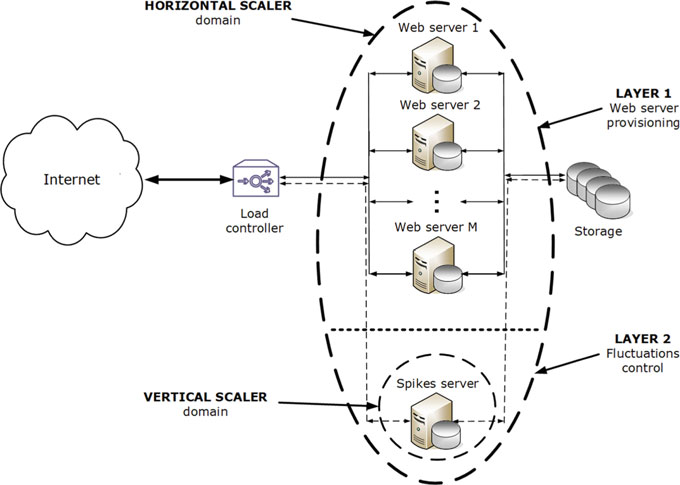
\includegraphics[width=1\textwidth]{system}
    \caption{Rappresentazione schematica dell'architettura ad alto livello dell'autoscaler gerarchico (ripresa da \cite[Fig.~6.8]{serazzi-jmt-book}).}
    \label{fig:system_architecture}
\end{figure}


\subsection{Componenti Logici dell'Infrastruttura}
Da una prospettiva puramente funzionale ed astratta, il sistema è composto da tre macro-moduli interconnessi che cooperano per elaborare il flusso di richieste in ingresso:
\begin{itemize}
    \item \textbf{Load Controller}: Rappresenta il punto di ingresso unico del datacenter. Questo modulo riceve l'intero flusso del traffico esterno e applica algoritmi di instradamento dinamico basati sullo stato istantaneo dei nodi di calcolo, agendo come decisore di prima istanza per l'allocazione del carico.
    \item \textbf{Cluster di Web Server}: È costituito da un pool di server standard destinati all'elaborazione del carico di lavoro convenzionale. Ciascun server assegna le proprie risorse hardware secondo logiche \textit{Processor Sharing}, tipiche dei server e della architetture di calcolo moderne, in cui la potenza di calcolo della CPU viene costantemente ripartita tra tutte le transazioni concorrenti in carico, evitando che singoli task monopolizzino il nodo.
    \item \textbf{Spike Server}: È una risorsa computazionale ad alta capacità mantenuta in uno stato di disponibilità elastica. Questo server non partecipa al bilanciamento ordinario del traffico, ma interviene esclusivamente come camera di compensazione quando i nodi del cluster principale si trovano in una condizione di congestione o stress critico.
\end{itemize}

\subsection{Dinamiche di Routing}
Il meccanismo che governa la deviazione dei flussi applicativi si basa sul concetto di \textbf{metrica reattiva istantanea}. Anzichè affidarsi a complessi e computazionalmente onerosi algoritmi di analisi predittiva delle serie storiche del traffico, l'orchestratore gestisce l'instradamento attraverso una sequenza logica a due stadi indipendenti, comune a qualsiasi stato di carico del sistema:
\begin{enumerate}
    \item \textbf{Selezione del Web Server}: All'arrivo di una nuova richiesta, il Load Controller applica preventivamente la politica di distribuzione principale per individuare un Web Server target all'interno del cluster.
    \item \textbf{Valutazione dello Spike Indicator}: Una volta determinato il server di destinazione, l'orchestratore ne interroga lo stato istantaneo estraendo lo \textit{Spike Indicator} $SI$, identificato nel numero esatto di richieste concorrenti che quel singolo nodo sta elaborando in quell'istante. Questa metrica viene confrontata istante per istante con la soglia critica di allarme $SI^{max}$.
\end{enumerate}

Il comportamento del router e la destinazione finale della richiesta seguono quindi una logica di controllo puramente reattiva e \textit{memoryless}: la decisione di instradamento viene presa per ogni singolo compito computazionale in tempo reale, basandosi esclusivamente sul valore puntuale di $SI$ osservato all'istante di campionamento. 
A seconda del risultato del confronto con la soglia d'allarme, si determinano due scenari di instradamento alternativi:

% DIAGRAMMA DI FLUSSO DEL PROCESSO DECISIONALE
\begin{figure}[htbp]
    \centering
    
    \usetikzlibrary{shapes.geometric, arrows, positioning, backgrounds}
    
    \begin{tikzpicture}[node distance=0.4cm and 0.5cm, auto]
        
        % Flusso dei nodi principali
        \node (inizio) [start] {Arrivo Richiesta};
        \node (routing) [process, right=of inizio] {Selezione Web\\Server Target};
        \node (scelta) [decision, right=of routing] {Valutazione\\$SI < SI^{max}$};
        
        % Destinazioni finali
        \node (ordinario) [webserver, above right=of scelta, yshift=-0.2cm] {\textbf{Scenario Ordinario}\\Esecuzione su Web Server scelto};
        \node (alto) [spikeserver, below right=of scelta, yshift=0.2cm] {\textbf{Stato Alto Carico}\\Dirottamento su Spike Server};
        
        % Connessioni lineari
        \draw [arrow] (inizio) -- (routing);
        \draw [arrow] (routing) -- (scelta);
        \draw [arrow] (scelta) |- node [near start, left, yshift=0.15cm] {Sì} (ordinario);
        \draw [arrow] (scelta) |- node [near start, left, yshift=-0.15cm] {No} (alto);
        
        \begin{scope}[on background layer]
            \node[draw=black!60, dashed, line width=0.8pt, rounded corners=4pt, fill=black!2, fit=(routing), inner sep=0.25cm, yshift=0.1cm] (lb_box) {};
            \node[above=0.02cm of lb_box, font=\scriptsize\sffamily\bfseries, text=black!80] {Load Controller};
        \end{scope}
        
    \end{tikzpicture}
    \caption{Diagramma di flusso sequenziale del processo decisionale e di routing.}
    \label{fig:routing_flowchart}
\end{figure}

\paragraph{Scenario Ordinario - $SI < SI^{max}$:}
Questo scenario si verifica nel momento in cui lo \textit{Spike Indicator} calcolato sul Web Server selezionato soddisfa la condizione di stabilità, indicando che l'intensità istantanea del traffico e le relative domande di servizio si mantengono entro i margini di capacità del nodo computazionale di linea. In questo caso, il Load Controller convalida l'affidabilità immediata del server target e vi immette direttamente la richiesta in ingresso per l'ordinaria esecuzione. Contestualmente, poichè la richiesta viene interamente presa in carico ed elaborata dal cluster di linea, lo \textit{Spike Server} non viene coinvolta nel flusso e permane in uno stato di quiescenza, ottimizzando l'efficienza energetica e computazionale complessiva del datacenter ed evitando lo spreco di risorse hardware.

\paragraph{Scenario di Alto Carico - $SI \ge SI^{max}$:}
Questo scenario si attiva nel momento esatto in cui il controllo rileva che l'occupazione istantanea del server target ha raggiunto o superato il limite di tolleranza, indicando l'insorgenza di un picco transitorio causato da un improvviso addensamento del tasso di arrivo o da un incremento imprevisto della complessità intrinseca dei task in esecuzione. Per prevenire un collasso prestazionale del \textit{Web Server} selezionato e il drastico innalzamento dei tempi di risposta, il modulo attiva immediatamente una deviazione d'emergenza, instradando la richiesta corrente verso lo \textit{Spike Server}. Di conseguenza, il \textit{Web Server} target sperimenta un'interruzione mirata dei nuovi arrivi che gli permette di operare in una modalità di svuotamento controllato, concentrando la potenza di calcolo esclusivamente sullo smaltimento dei processi precedentemente presi in carico; in questo modo, lo \textit{Spike Indicator} decresce progressivamente man mano che i task completano l'esecuzione e abbandonano la stazione. Contestualmente, lo \textit{Spike Server}, caratterizzato da un'elevata capacità computazionale e da logiche di scaling verticale, si fa carico dell'intero surplus di traffico fungendo da camera di compensazione e assorbendo l'impatto stocastico del picco. Questo isolamento garantisce che il carico accumulato sul Web Server principale non degradi le prestazioni dei nuovi arrivi, smorzando la varianza e il valore medio del tempo di risposta globale del sistema. Il dirottamento applicato alle nuove richieste decade poi istantaneamente non appena un successivo arrivo campiona un valore dello \textit{Spike Indicator} ritornato strettamente al di sotto della soglia di sicurezza $SI^{max}$, ripristinando la normale allocazione sul cluster di linea.


\subsection{Logiche di Scaling}
L'efficienza complessiva dell'architettura gerarchica risiede nella cooperazione strategica e coordinata tra le politiche di \textbf{routing reattivo} e le logiche di \textbf{autoscaling delle risorse}: questi due sistemi non operano come entità isolate, ma si integrano sinergicamente su piani strutturali e scale temporali marcatamente differenziate per proteggere l'infrastruttura. Se da un lato il routing interviene istante per istante a livello microscopico, dall'altro lato i meccanismi di scaling adattano dinamicamente la topologia e la capacità hardware del sistema per assorbire i carichi sul lungo e sul breve termine.

\paragraph{Scaler Orizzontale:}
Questa logica agisce sulla dimensionalità quantitativa del cluster principale e opera su una scala temporale macroscopica a bassa frequenza, erigendosi a presidio delle variazioni strutturali e a lungo termine del traffico. Il meccanismo valuta la necessità di ridimensionare il pool di linea monitorando costantemente il tempo medio di risposta delle richieste, calcolato all'interno di una finestra temporale mobile; l'adozione di tale media mobile si rivela fondamentale per filtrare il rumore stocastico e prevenire reazioni premature a fluttuazioni transitorie. Quando il tempo medio di risposta supera la soglia di sbarramento superiore $R^{max}$ e il periodo di vincolo temporale dall'ultima riconfigurazione è completamente esaurito, l'orchestratore dispone l'allocazione e l'integrazione immediata di un nuovo server nel cluster per ripristinare i livelli di servizio attesi. Al contrario, qualora la metrica basata sulla finestra mobile si attesti stabilmente al di sotto della soglia inferiore $R^{min}$, il sistema pianifica la dismissione delle risorse in esubero per minimizzare i costi operativi. Al fine di preservare la continuità del servizio e non penalizzare le transazioni in corso, la contrazione della capacità applica una rigida politica di svuotamento controllato: il nodo designato alla rimozione viene immediatamente rimosso dalle rotazioni del Load Controller per bloccare l'ingresso di nuovi flussi, ma viene mantenuto alimentato ed attivo il tempo necessario a consentire il totale completamento di tutti i processi precedentemente presi in carico e rimasti pendenti nella sua coda.

% =========================================================================
% DIAGRAMMA AUTOSCALING ORIZZONTALE
% =========================================================================
\begin{figure}[!h]
    \centering
    \usetikzlibrary{shapes.geometric, arrows, positioning}
    
    \begin{tikzpicture}[node distance=0.6cm and 1.2cm, auto]
        
        % Flusso principale
        \node (inizio) [start] {Valutazione Periodica};
        \node (metric) [process, below=of inizio] {Calcolo Tempo Risposta\\su Finestra Mobile};
        \node (cooldown) [decision, below=of metric, yshift=-0.1cm] {Cooldown\\Scaduto?};
        \node (scelta) [decision, below=of cooldown, yshift=-0.2cm] {Verifica\\Soglie};
        \node (nessuna) [start, below=of scelta, yshift=-0.4cm] {Nessuna Azione};
        
        % Esiti laterali
        \node (scaleout) [spikeserver, left=of scelta, xshift=-0.2cm] {\textbf{Scale-Out}\\Aggiunta Server al Cluster};
        \node (scalein) [webserver, right=of scelta, xshift=0.2cm] {\textbf{Scale-In}\\Rimozione con Svuotamento};
        
        % Connessioni lineari e bivi
        \draw [arrow] (inizio) -- (metric);
        \draw [arrow] (metric) -- (cooldown);
        \draw [arrow] (cooldown) -- node [near start, right] {Sì} (scelta);
        \draw [arrow] (cooldown.east) -- node [near start, above] {No} ([xshift=1.0cm]cooldown.east -| scalein.east) |- (nessuna.east);
        
        % Frecce dal blocco decisionale delle soglie
        \draw [arrow] (scelta.west) -- node [near start, above] {$\ge R^{max}$} (scaleout.east);
        \draw [arrow] (scelta.east) -- node [near start, above] {$\le R^{min}$} (scalein.west);
        
        % Testo "Altrimenti" posizionato a lato della freccia inferiore
        \draw [arrow] (scelta.south) -- (nessuna.north);
        \node [right=0.05cm of scelta.south, yshift=-0.3cm, font=\small] {Altrimenti};
        
    \end{tikzpicture}
    \caption{Logica di monitoraggio e processo decisionale dell'autoscaling orizzontale.}
    \label{fig:horizontal_scaler_flowchart}
\end{figure}

\paragraph{Scaler Verticale:}
Questa logica interviene sulla capacità computazionale qualitativa dell'unità di riserva e opera su una scala temporale microscopica ad attivazione immediata, rispondendo alle repentine e violente variazioni indotte dai picchi di traffico ad alta frequenza. Il meccanismo di controllo agisce in modo dinamico modulando la quota di capacità hardware dedicata allo Spike Server (il moltiplicatore di velocità della CPU) in base al carico istantaneo, valutato direttamente in termini di numero assoluto di richieste concorrenti simultaneamente attive all'interno della sua stazione. Nel momento esatto in cui il volume di task deviati e presi in carico dall'unità ausiliaria eguaglia o supera una determinata soglia limite superiore, e nel rispetto del tempo di sosta imposto dal relativo \textit{cooldown}, l'ottimizzatore verticale interviene istantaneamente incrementando la potenza dio calcolo allocata per accelerare i tempi di soddisfacimento dei processi d'emergenza. Questa accelerazione funge da scudo immediato e temporaneo, assorbendo il picco transitorio senza la necessità di attendere i lunghi tempi di boot tipici del provisioning orizzontale. Non appena la pressione stocastica si attenua e lo svuotamento delle code fa flettere il numero di richieste attive al di sotto della soglia di rilascio inferiore, il sistema revoca l'assegnazione straordinaria di risorse ripristinando il moltiplicatore di velocità alla sua configurazione di base, riducendo istantaneamente l'impronta economica e salvaguardando l'efficienza energetica del datacenter.

% =========================================================================
% DIAGRAMMA AUTOSCALING VERTICALE
% =========================================================================
\begin{figure}[H]
    \centering
    \usetikzlibrary{shapes.geometric, arrows, positioning}
    
    \begin{tikzpicture}[node distance=0.6cm and 1.2cm, auto]
        
        % Flusso principale
        \node (inizio) [start] {Campionamento Carico};
        \node (metric) [process, below=of inizio] {Conteggio Richieste\\Attive su Spike Server};
        \node (cooldown) [decision, below=of metric, yshift=-0.1cm] {Cooldown\\Scaduto?};
        \node (scelta) [decision, below=of cooldown, yshift=-0.2cm] {Verifica\\Soglie Load?};
        \node (nessuna) [start, below=of scelta, yshift=-0.4cm] {Nessuna Azione};
        
        % Esiti laterali
        \node (scaleup) [spikeserver, left=of scelta, xshift=-0.2cm] {\textbf{Scale-Up}\\Incremento CPU Multiplier};
        \node (scaledown) [webserver, right=of scelta, xshift=0.2cm] {\textbf{Scale-Down}\\Ripristino Base Speed};
        
        % Connessioni lineari e bivi
        \draw [arrow] (inizio) -- (metric);
        \draw [arrow] (metric) -- (cooldown);
        \draw [arrow] (cooldown) -- node [near start, right] {Sì} (scelta);
        \draw [arrow] (cooldown.east) -- node [near start, above] {No} ([xshift=1.0cm]cooldown.east -| scaledown.east) |- (nessuna.east);
        
        % Frecce dal blocco decisionale delle soglie
        \draw [arrow] (scelta.west) -- node [near start, above] {$\ge$ Upper} (scaleup.east);
        \draw [arrow] (scelta.east) -- node [near start, above] {$\le$ Lower} (scaledown.west);
        
        % Testo "Altrimenti"
        \draw [arrow] (scelta.south) -- (nessuna.north);
        \node [right=0.05cm of scelta.south, yshift=-0.3cm, font=\small] {Altrimenti};
        
    \end{tikzpicture}
    \caption{Processo di modulazione della capacità computazionale gestito dall'autoscaling verticale.}
    \label{fig:vertical_scaler_flowchart}
\end{figure}

\clearpage


% =========================================================================
% OBIETTIVI
% =========================================================================
\section{Obiettivi del Progetto}
La progettazione e lo sviluppo del simulatore a eventi discreti oggetto del presente studio sono orientati alla definizione, quantificazione e validazione empirica delle metriche analitiche e prestazionali che governano l'infrastruttura gerarchica proposta. L'obiettivo fondamentale della ricerca risiede nella dimostrazione, condotta attraverso un rigoroso approccio sperimentale, dell'efficacia derivante dalla stretta cooperazione e sinergia tra le decisioni di \textbf{routing reattivo istantaneo} (operate al Layer 2 dal Load Controller) e i meccanismi di \textbf{adattamento dinamico delle risorse} (attuati tramite le logiche di scaling orizzontale e verticale). 

Attraverso la riproduzione di scenari sintetici caratterizzati da differenti intensità stocastiche e coefficienti di variabilità del traffico, la campagna di simulazione mira a mappare le interdipendenze tra l'allocazione hardware e la degradazione dei tempi di risposta. Questo percorso metodologico si articola in tre macro-aree di indagine sequenziali e strettamente interconnesse, orientate rispettivamente al dimensionamento ottimale dei parametri operativi, all'analisi di sensibilità economica e computazionale del sistema in contesti sia dinamici che stazionari, e infine all'introduzione di meccanismi ottimizzati per l'abbattimento dei fenomeni di instabilità computazionale nei casi limite.


\subsection{Dimensionamento Infrastrutturale}
La fase di dimensionamento si occupa di identificare la configurazione strutturale ottimale e i parametri operativi di base necessari a garantire che l'infrastruttura sia in grado di sostenere i livelli di traffico attesi, massimizzando l'efficienza hardware. In particolare, l'intero processo di calibrazione parametrica è guidato dal vincolo di progetto di mantenere un valore target massimo del tempo di risposta globale del sistema impostato rigorosamente a 6 secondi. Tale soglia critica rappresenta il limite di tolleranza oltre il quale il sistema viene considerato in uno stato di degradazione prestazionale, e funge da benchmark fondamentale per valutare l'efficacia delle decisioni di routing e delle soglie di intervento dei moduli di autoscaling.

\paragraph{Politiche di Instradamento:}
L'obiettivo primario sul piano della ripartizione del traffico risiede nella valutazione comparativa e quantitativa di diverse discipline stocastiche e deterministiche di bilanciamento del carico. Attraverso la campagna di simulazione, si intende analizzare in che misura l'adozione di differenti algoritmi influenzi la distribuzione dei job all'interno del cluster ordinario, indipendentemente dallo \textit{Spike Server}. L'indagine mira a identificare la politica di routing ottimale capace di minimizzare la formazione di code e l'insorgenza di fenomeni di sbilanciamento locale, garantendo un utilizzo equo delle risorse di linea e concorrendo attivamente alla riduzione del tasso di attivazione del meccanismo di dirottamento verso lo Spike Server.

\paragraph{Calibrazione dello Scaling Verticale:}
In questo contesto, la ricerca si prefigge di validare l'efficacia e la stabilità della strategia di adattamento verticale applicata all'unità ausiliaria di gestione dei picchi. L'obiettivo si focalizza sulla calibrazione precisa dei parametri operativi che governano la capacità di questa risorsa di variare istantaneamente la propria potenza computazionale, modulando il moltiplicatore di velocità della CPU in risposta al superamento delle soglie di carico stimate. L'analisi punta a verificare la capacità di tale scudo ad alta frequenza nel contenere le derive della latenza e della coda nei transitori critici in cui il cluster principale sperimenta una saturazione temporanea.

\paragraph{Dimensionamento dello Scaling Orizzontale:}
L'obiettivo è l'identificazione e il dimensionamento accurato dei parametri macroscopici che regolano la variazione della numerosità dei server attivi nel cluster principale. Sfruttando l'approccio empirico della simulazione, si intendono determinare le soglie critiche ottimali di aggiunta e di rimozione delle istanze computazionali, basate sulle metriche temporali aggregate ed elaborate tramite la finestra mobile. La ricerca è volta a definire una configurazione topologica bilanciata, capace di rispondere con agilità e precisione a variazioni di carico strutturali e sostenute nel tempo, minimizzando sia i ritardi di provisioning che potrebbero esporre il sistema a congestioni prolungate incompatibili con il target prestazionale, sia i fenomeni di instabilità o oscillazioni della capacità hardware.


\subsection{Analisi delle Prestazioni}
In questa fase si procede a una valutazione approfondita e sistematica delle prestazioni computazionali e dei costi operativi dell'infrastruttura, esaminandone il comportamento sia in contesti dinamici fortemente perturbati sia in condizioni stazionarie di regime. L'obiettivo centrale di questa indagine è verificare se, applicando i parametri operativi calibrati nella precedente fase di dimensionamento, l'infrastruttura sia effettivamente in grado di garantire e mantenere i Quality of Service attesi sul tempo di risposta globale. Contestualmente, l'analisi si propone di quantificare l'efficienza della soluzione proposta attraverso una valutazione comparativa dell'impatto economico, misurando i benefici finanziari e strutturali che si ottengono dall'adozione dello scaler gerarchico rispetto a una strategia rigida di provisioning fisso delle risorse.

\paragraph{Analisi dei Costi e Trade-off Economico:}
Viene condotta un'analisi economica orientata alla quantificazione del \textit{trade-off} vincolante tra i costi operativi infrastrutturali e il guadagno prestazionale ottenuto. L'obiettivo finale consiste nell'individuare un punto di equilibrio ottimale che permetta di minimizzare la spesa operativa totale del datacenter, dimostrando la sostenibilità economica dello scaling gerarchico rispetto ai costi ridondanti legati a un provisioning fisso, pur garantendo il rispetto del vincolo del tempo di risposta entro il target stabilito per l'utente finale.

\paragraph{Analisi Transitoria e Dinamica dei Sistemi:}
L'indagine focalizzata sulle dinamiche transitorie del sistema viene condotta avviando deliberatamente l'ambiente di simulazione in uno stato completamente vuoto e inattivo. Questo approccio metodologico, basato sull'inizializzazione a zero delle code e delle risorse computazionali, si rivela indispensabile per mappare l'evoluzione temporale del sistema fuori dal regime e determinare con precisione l'istante di convergenza in cui l'infrastruttura raggiunge la stabilità operativa. Lo studio del transitorio iniziale permette così di quantificare la durata della fase di \textit{warm-up}, necessaria affinchè le metriche prestazionali si liberino dal bias delle condizioni iniziali, e di misurare empiricamente il tempo di reazione e i ritardi di adattamento dei moduli hardware a seguito dell'immissione del traffico stocastico. L'analisi consente infine di sottoporre a stress test il coordinamento microscopico tra i meccanismi di routing e le soglie di attivazione degli scaler proprio nelle fasi più volatili e critiche di avvio, verificando la tempestività dell'intero impianto gerarchico nel preservare i QoS legati alla latenza prima del consolidamento del regime stazionario.

\paragraph{Analisi in Stato Stazionario:}
Una volta esauriti completamente gli effetti dei transitori di avvio e superata la fase di warm-up, l'obiettivo si sposta sulla caratterizzazione e sulla verifica empirica del comportamento del sistema in stato stazionario. Questa indagine è finalizzata a osservare e validare le risposte operative e le prestazioni dell'infrastruttura a regime sotto l'effetto dei parametri strutturali precedentemente deliberati. Attraverso il monitoraggio puntuale di indicatori chiave, quali il livello di utilizzazione media dello Spike Server e il tempo medio di risposta stabilizzato, lo studio si propone di confermare che la configurazione architetturale selezionata sia in grado di sostenere i tassi di arrivo costanti nel lungo periodo. L'analisi mira a certificare la robustezza intrinseca del sistema e la convergenza asintotica dei Quality of Service ai valori nominali di progetto, garantendo la stabilità dei flussi anche in presenza di sorgenti di traffico affette da un'elevata variabilità stocastica.


\subsection{Mitigazione dell'Instabilità}
L'ultima macro-area di indagine si concentra su una proposta evolutiva del sistema attraverso l'introduzione di logiche algoritmiche ottimizzate, ingegnerizzate specificamente per la stabilizzazione dei controlli nei casi limite e negli scenari di transizione critica.

\paragraph{Meccanismo di Controllo a Soglie Differenziate:}
L'obiettivo conclusivo del progetto risiede nella valutazione empirica di una soluzione migliorativa volta a ottimizzare la gestione dei fenomeni di saturazione sui singoli nodi computazionali. Nello specifico, si analizza lo scenario fortemente critico in cui un Web Server del cluster si trova a operare in stretta prossimità della soglia di allarme dello \textit{Spike Indicator} $SI^{max}$: in assenza di contromisure, la natura stocastica e l'arrivo ravvicinato di molteplici richieste potrebbero provocare repentine oscillazioni nelle decisioni di routing. Questo fenomeno di instabilità decisionale rischierebbe di indurre continui e sterili cicli di attivazione e disattivazione del dirottamento, con il potenziale effetto di degradare le prestazioni generali e mantenere il server in uno stato di micro-congestione inefficiente. La ricerca intende quindi investigare se l'introduzione di un meccanismo a doppia soglia di tolleranza, governato dall'azione combinata della soglia critica superiore $SI^{max}$ e di una potenziale soglia di rilascio inferiore $SI^{min}$, consenta effettivamente di stabilizzare le scelte del router. Lo studio mira a osservare come la definizione di questo intervallo di transizione controllato influenzi lo smorzamento delle fluttuazioni ad alta frequenza, analizzando l'impatto reale che tale logica esercita sulla fluidità di gestione del traffico eccedente, sulla linearità dei QoS e sul tempo di risposta globale del sistema, a fronte di un ipotizzabile incremento nel tasso di utilizzazione dello Spike Server in condizioni di carico limite.

\clearpage


% =========================================================================
% MODELLO CONCETTUALE
% =========================================================================
\section{Modellazione Concettuale del Sistema}
Il sistema viene formalizzato come una rete aperta di code operante in parallelo, all'interno della quale i flussi applicativi complessivi, caratterizzati da un tasso di arrivo globale $\lambda$, vengono intercettati ed orchestrati da un'unità centrale di controllo e indirizzati ai vari centri di servizio.

% =========================================================================
% DIAGRAMMA DELLA RETE DI CODE
% =========================================================================
\begin{figure}[htbp]
    \centering
    \usetikzlibrary{shapes.geometric, arrows, positioning, backgrounds}
    
    \begin{tikzpicture}[node distance=0.5cm and 1.2cm, auto, >=stealth, line width=0.8pt]
        
        % -----------------------------------------------------------------
        % STILI DEI NODI
        % -----------------------------------------------------------------
        \tikzset{
            lb_node/.style={circle, draw=teal!80, fill=teal!8, minimum size=1.5cm, font=\small\sffamily\bfseries, align=center},
            srv_web/.style={circle, draw=cyan!80, fill=cyan!8, minimum size=0.9cm, font=\small\sffamily},
            srv_spike/.style={circle, draw=orange!80, fill=orange!8, minimum size=0.9cm, font=\small\sffamily},
            arrow/.style={->, draw=gray!90, thick},
            line/.style={draw=gray!90, thick}
        }

        % Ingresso del sistema
        \coordinate (ingresso) at (-2, 0);
        
        % Nodo Load Controller
        \node (lb) [lb_node] at (0,0) {Load\\Controller};
        
        % Bus di smistamento ortogonale
        \coordinate (bus_x) at (2.2, 0);

        % =================================================================
        % CLUSTER WEB SERVERS
        % =================================================================
        
        % Posizionamento nodi Server
        \node (s1) [srv_web] at (5.8, 3.5) {$\mu_{web}$};
        \node (s2) [srv_web] at (5.8, 2.3) {$\mu_{web}$};
        \node (sm) [srv_web] at (5.8, 0.3) {$\mu_{web}$};
        
        % Punti di sospensione verticali
        \node at (5.0, 1.4) [font=\LARGE\bfseries, text=gray!60] {$\vdots$};
        
        % Coda Web 1
        \coordinate (in_s1) at ([xshift=-1.2cm]s1.west);
        \draw[cyan!80, thick] (in_s1) ++(0,0.3) -- ++(1.2,0) -- ++(0,-0.6) -- ++(-1.2,0);
        \draw[cyan!70] (in_s1) ++(0,0.15) -- ++(1.2,0);
        \draw[cyan!70] (in_s1) ++(0,0.0) -- ++(1.2,0);
        \draw[cyan!70] (in_s1) ++(0,-0.15) -- ++(1.2,0);

        % Coda Web 2
        \coordinate (in_s2) at ([xshift=-1.2cm]s2.west);
        \draw[cyan!80, thick] (in_s2) ++(0,0.3) -- ++(1.2,0) -- ++(0,-0.6) -- ++(-1.2,0);
        \draw[cyan!70] (in_s2) ++(0,0.15) -- ++(1.2,0);
        \draw[cyan!70] (in_s2) ++(0,0.0) -- ++(1.2,0);
        \draw[cyan!70] (in_s2) ++(0,-0.15) -- ++(1.2,0);

        % Coda Web M
        \coordinate (in_sm) at ([xshift=-1.2cm]sm.west);
        \draw[cyan!80, thick] (in_sm) ++(0,0.3) -- ++(1.2,0) -- ++(0,-0.6) -- ++(-1.2,0);
        \draw[cyan!70] (in_sm) ++(0,0.15) -- ++(1.2,0);
        \draw[cyan!70] (in_sm) ++(0,0.0) -- ++(1.2,0);
        \draw[cyan!70] (in_sm) ++(0,-0.15) -- ++(1.2,0);
        
        % Connessioni dal Bus alle code Web
        \draw[arrow] (2.2, 3.5) -- (in_s1);
        \draw[arrow] (2.2, 2.3) -- (in_s2);
        \draw[arrow] (2.2, 0.3) -- (in_sm);
        
        % Collettore uscite Web Servers
        \coordinate (exit_web) at (8.5, 1.9);
        \draw[line] (s1.east) -- (7.2, 3.5);
        \draw[line] (s2.east) -- (7.2, 2.3);
        \draw[line] (sm.east) -- (7.2, 0.3);
        \draw[line] (7.2, 3.5) -- (7.2, 0.3); 
        \draw[arrow] (7.2, 1.9) -- (exit_web);

        % =================================================================
        % SPIKE SERVER
        % =================================================================
        
        % Posizionamento nodo Spike Server
        \node (s_spike) [srv_spike] at (5.8, -2.5) {$\mu_{spike}$};
        
        % Coda Spike
        \coordinate (in_spike) at ([xshift=-1.2cm]s_spike.west);
        \draw[orange!80, thick] (in_spike) ++(0,0.3) -- ++(1.2,0) -- ++(0,-0.6) -- ++(-1.2,0);
        \draw[orange!70] (in_spike) ++(0,0.15) -- ++(1.2,0);
        \draw[orange!70] (in_spike) ++(0,0.0) -- ++(1.2,0);
        \draw[orange!70] (in_spike) ++(0,-0.15) -- ++(1.2,0);
        
        % Connessione dal Bus alla coda Spike
        \draw[arrow] (2.2, -2.5) -- (in_spike);
        \coordinate (exit_spike) at (8.5, -2.5);
        \draw[arrow] (s_spike.east) -- (exit_spike);

        % =================================================================
        % RECTANGLES & LABEL
        % =================================================================
        \begin{scope}[on background layer]
            % Evidenziazione Pool Web Server
            \draw[draw=cyan!60, dashed, fill=cyan!3, line width=1.2pt, rounded corners=10pt] (3.7, -0.4) rectangle (6.6, 4.2);
            \node at (5.15, 4.5) [font=\small\sffamily\bfseries, text=cyan!80!black] {Web Servers Pool};

            % Evidenziazione Spike Server
            \draw[draw=orange!60, dashed, fill=orange!3, line width=1.2pt, rounded corners=10pt] (3.7, -3.3) rectangle (6.6, -1.7);
            \node at (5.15, -1.4) [font=\small\sffamily\bfseries, text=orange!80!black] {Spike Server};
        \end{scope}

        % -----------------------------------------------------------------
        % LINEA PRINCIPALE
        % -----------------------------------------------------------------
        \draw[arrow] (ingresso) -- node[above=0.05cm, font=\large] {$\lambda$} (lb.west);
        \draw[line] (lb.east) -- (2.2, 0);
        \draw[line] (2.2, 3.5) -- (2.2, -2.5);

    \end{tikzpicture}
    \caption{Modello concettuale a reti di code parallele.}
    \label{fig:conceptual_queueing_model}
\end{figure}


\subsection{Caratterizzazione dei Centri di Servizio}
Ciascun componente strutturale viene astratto come un preciso centro di servizio, definito univocamente dalle proprie variabili di stato, capacità di memorizzazione e algebra di ripartizione della risorsa computazionale.

\begin{itemize}
    \item \textbf{Load Controller:} Viene modellato concettualmente come un centro a servizio istantaneo e capacità di accumulo nulla. Non possiede code di attesa nè servitori reali; agisce esclusivamente come operatore di scomposizione e indirizzamento del flusso poissoniano globale in ingresso, avente tasso di arrivo $\lambda$. La sua unica funzione nel modello è ripartire il tasso di ingresso ai vari centri in base alle politiche di routing.

    \item \textbf{Pool dei Web Server:} Costituito da un insieme di $N(t)$ stazioni di servizio parallele, disaccoppiate e indipendenti, dove la numerosità dei nodi attivi è regolata nel lungo termine dall'ottimizzatore orizzontale. Dal punto di vista analitico, ciascun nodo del pool è formalizzato come una stazione a capacità di accodamento infinita e a singolo servente. La disciplina di servizio implementata è il \textit{Processor Sharing}: ciò implica che il tasso di servizio nominale del server, pari a $\mu_{web}$, venga costantemente e uniformemente suddiviso tra tutti i job $k_i(t)$ simultaneamente residenti all'interno della stazione.

    \item \textbf{Spike Server:} Viene astratto come una stazione di servizio singola a capacità illimitata, isolata topologicamente e operante anch'essa sotto disciplina \textit{Processor Sharing} per garantire l'omogeneità analitica dei tempi di sosta. La peculiarità computazionale di questo centro risiede nell'elasticità del proprio parametro di servizio, il quale non è costante bensì tempo-variante: $\mu_{spike}(t) = \kappa(t) \cdot \mu_{base}$, dove $\kappa(t) \in \mathbb{N}^+$ rappresenta il moltiplicatore discreto della capacità elaborativa imposto dalle decisioni dello scaling verticale. Il centro è caratterizzato da un tasso di arrivo intermittente, nullo in condizioni nominali e attivato esclusivamente al superamento delle soglie critiche del pool superiore.
\end{itemize}


\subsection{Definizione dello Stato del Sistema}
Lo stato del sistema al tempo $t$ è formalizzato attraverso un vettore esteso di variabili aleatorie e deterministiche, in grado di mappare compiutamente sia l'occupazione fisica delle risorse computazionali, sia lo stato interno dei moduli di controllo e monitoraggio:
\begin{equation}
    S(t) = \left\{ N(t), \mathbf{n}(t), n_s(t), v_s(t), \hat{W}_{mw}(t), \tau_h(t), \tau_v(t) \right\}
\end{equation}

La componente legata all'infrastruttura hardware e all'allocazione del carico è descritta dalle seguenti variabili:
\begin{itemize}
    \item $N(t) \in \{N_{min}, \dots, N_{max}\}$ rappresenta la numerosità istantanea dei Web Server attivi nel cluster di linea, governata dallo scaling orizzontale.
    \item $\mathbf{n}(t) = (n_1(t), n_2(t), \dots, n_{N(t)}(t))$ indica il vettore del carico corrente del pool, in cui ciascuna componente $n_i(t) \in \mathbb{N}$ esprime il numero di richieste concorrenti in fase di elaborazione all'interno del server $i$-esimo.
    \item $n_s(t) \in \mathbb{N}$ rappresenta la quantità di task simultaneamente presi in carico e in fase di processamento presso lo Spike Server.
    \item $v_s(t) \in \{v_{base}, v_{speed}\}$ definisce il moltiplicatore di velocità applicato alla capacità elaborativa della stazione di picco, modulato dalle decisioni dello scaling verticale.
\end{itemize}

Le variabili di controllo, necessarie per tracciare la memoria storica dell'algoritmo e determinare l'evoluzione dei controllori, sono invece definite come:
\begin{itemize}
    \item $\hat{W}_{mw}(t) \in \mathbb{R}^+$ indica la stima del tempo medio di risposta globale del sistema, calcolata dinamicamente sull'orizzonte temporale della finestra mobile attiva al tempo $t$, che funge da metrica di input per la logica di scaling orizzontale.
    \item $\tau_h(t) \in \mathbb{R}^+$ esprime il tempo di \textit{cooldown} residuo per l'autoscaling orizzontale; se $\tau_h(t) > 0$, qualsiasi azione di \textit{Scale-Out} o \textit{Scale-In} viene temporaneamente inibita, e il timer decade linearmente con il progredire del tempo.
    \item $\tau_v(t) \in \mathbb{R}^+$ definisce il tempo di \textit{cooldown} residuo associato al modulo di scaling verticale dell'unità ausiliaria, agendo come vincolo temporale per impedire oscillazioni ad alta frequenza sul moltiplicatore di velocità dello Spike Server.
\end{itemize}


\subsection{Transizioni di Stato}
L'evoluzione dinamica del vettore di stato $S(t)$ è regolata dalle leggi microscopiche che governano il processamento dei job, l'instradamento dei flussi e i trigger di attivazione dei controllori.

\paragraph{Evoluzione del Tasso di Servizio:}
All'interno di ciascuna stazione attiva (sia essa un Web Server $i$ o lo Spike Server), l'effettivo tasso di completamento unitario non è costante, ma evolve in modo asincrono a ogni transizione del carico locale. Definita la capacità nominale del centro, il tasso di servizio istantaneo erogato dal singolo servitore logico al task generico è condizionato inversamente dallo stato di occupazione del centro stesso:
\begin{equation}
    \mu_{i}(t) = \frac{\mu_{web}}{n_i(t)}, \quad \mu_{s}(t) = \frac{v_s(t) \cdot \mu_{base}}{n_s(t)}
\end{equation}

\paragraph{Transizioni nei Moduli di Scaling:}
Le variazioni delle variabili di controllo dello stato avvengono su scale temporali disaccoppiate e secondo logiche distinte:
\begin{itemize}
    \item \textbf{Transizioni Orizzontali:} La mutazione della topologia del cluster, ovvero $\Delta N(t) = \pm 1$, avviene su eventi discreti. Essa è subordinata alla doppia condizione di azzeramento del timer residuo, che si ottiene con $\tau_h(t) = 0$, e di superamento delle soglie da parte della variabile $\hat{W}_{mw}(t)$.
    \item \textbf{Transizioni Verticali:} La variabile $v_s(t)$ scala tra i livelli discreti delle velocità in funzione del variare della componente di stato $n_s(t)$ (sempre secondo delle soglie impostate), a patto che il rispettivo timer di blocco verifichi la condizione $\tau_v(t) = 0$.
\end{itemize}


\subsection{Analisi degli Eventi Discreti}
L'evoluzione temporale del modello è orchestrata da un motore di simulazione a eventi discreti, in cui lo stato del sistema muta esclusivamente in corrispondenza di istanti temporali isolati e asincroni. Poiché l'infrastruttura implementa una disciplina di servizio \textit{Processor Sharing}, i tempi di uscita dal sistema non dipendono unicamente dalla domanda di servizio originaria del job; di conseguenza, il simulatore è vincolato a ricalcolare dinamicamente e a rischedulare i futuri eventi di fine elaborazione a ogni transizione di stato che modifichi i vettori di carico $n_i(t)$ o $n_s(t)$.

Il ciclo di vita della simulazione è governato da tre tipologie fondamentali di eventi operativi:

\begin{enumerate}
    \item \textbf{Evento di Arrivo:} 
    Identifica l'immissione di una nuova richiesta nel sistema secondo il tasso stocastico $\lambda$. Il Load Controller intercetta l'evento ed esegue istantaneamente l'algoritmo di routing e il controllo a soglie differenziate, assegnando il job al Web Server candidato $i$ o all'unità di riserva. Questa transizione incrementa la variabile di carico corrispondente $n_i(t) \leftarrow n_i(t) + 1$ oppure $n_s(t) \leftarrow n_s(t) + 1$, provocando la ridefinizione immediata della quota computazionale spettante ai task concorrenti e l'aggiornamento dei rispettivi tempi di completamento stimati.

    \item \textbf{Evento di Completamento:} 
    Segnala la fine del processamento di un job all'interno di un centro di servizio. L'evento determina il decremento unitario della variabile di occupazione del rispettivo nodo, $n_i(t) \leftarrow n_i(t) - 1$ oppure $n_s(t) \leftarrow n_s(t) - 1$,  e la contestuale rimozione del job dal sistema. In questa esatta transizione, il simulatore effettua il campionamento della metrica sul tempo di risposta individuale, ne invia il valore al modulo della finestra mobile e rimodula al rialzo la velocità di elaborazione per i task rimasti all'interno della stazione.

    \item \textbf{Evento Periodico di Monitoraggio:} 
    Rappresenta un evento di clock deterministico e ricorrente, totalmente disaccoppiato dai flussi di traffico. Al verificarsi di questo trigger, gli agenti di controllo analizzano i valori assunti dalle metriche aggregate memorizzate nello stato, specificamente il tempo medio di risposta globale sulla finestra mobile $\hat{W}_{mw}(t)$ e l'occupazione della risorsa di picco $n_s(t)$, per valutare l'opportunità di variare la topologia del cluster $N(t)$ o lo \textit{speedup} verticalizzato $v_s(t)$, aggiornando i relativi vettori dei cooldown qualora un'azione di scaling venga effettivamente validata e rischedulando un evento di monitoraggio ad una distanza pari proprio al cooldown.
\end{enumerate}

\clearpage


\section{Modello delle Specifiche}
Il modello delle specifiche definisce in modo puntuale i parametri operativi, le variabili di controllo e gli indici di prestazione che caratterizzano il sistema simulato, fornendo una base quantitativa per l'analisi dei risultati.

\subsection{Variabili di Ingresso e Carico (Workload)}
Il carico di lavoro è modellato come un processo stocastico caratterizzato dalle seguenti grandezze:
\begin{itemize}
    \item \textbf{Tasso di Arrivo ($\lambda$)}: Rappresenta il numero medio di richieste al secondo che entrano nel sistema. L'intertempo tra gli arrivi ($\tau$) segue distribuzioni statistiche variabili in base allo scenario di test (es. Esponenziale per traffico regolare, Iperesponenziale per traffico \textit{bursty}).
    \item \textbf{Coefficiente di Variazione degli Arrivi ($CV_a$)}: Utilizzato per modellare la variabilità e la dispersione degli interarrivi, fondamentale per lo studio della robustezza al burstiness.
    \item \textbf{Tempo di Servizio Medio ($E[S]$)}: La domanda di servizio media di ogni job, espressa in secondi di tempo CPU.
    \item \textbf{Coefficiente di Variazione del Servizio ($CV_s$)}: Definisce l'eterogeneità della complessità computazionale dei job.
\end{itemize}

\subsection{Parametri di Configurazione del Sistema}
L'infrastruttura è governata da un insieme di costanti e soglie decisionali che ne determinano il comportamento dinamico:
\begin{itemize}
    \item \textbf{Configurazione del Cluster}: 
    \begin{itemize}
        \item $N_{min}, N_{max}$: Limiti inferiore e superiore al numero di Web Server attivi nel cluster.
        \item $COOLDOWN$: Intervallo di tempo minimo tra due azioni consecutive di scaling orizzontale, necessario per evitare instabilità strutturali.
    \end{itemize}
    \item \textbf{Soglie di Instradamento (Routing)}:
    \begin{itemize}
        \item $SI_{max}$ (\textit{Spike Indicator Max}): Soglia di carico oltre la quale un server devia il traffico verso l'unità di picco.
        \item $SI_{low}$ (\textit{Spike Indicator Low}): Soglia di ripristino per il ritorno allo stato operativo normale.
    \end{itemize}
    \item \textbf{Parametri di Scaling}:
    \begin{itemize}
        \item $R^{max}, R^{min}$: Soglie temporali (sul tempo di risposta medio) per attivare rispettivamente lo \textit{Scale Out} e lo \textit{Scale In}.
        \item $\Delta v_s$: Incremento discreto applicato al moltiplicatore di velocità dello Spike Server durante l'adattamento verticale.
    \end{itemize}
\end{itemize}

\subsection{Indici di Prestazione (Performance Indices)}
L'efficacia del sistema è valutata attraverso il monitoraggio dei seguenti indici di uscita:
\begin{itemize}
    \item \textbf{Tempo di Risposta Medio ($R_0$)}: Tempo totale trascorso da un job nel sistema (attesa + elaborazione). Rappresenta la metrica principale per la verifica degli SLA.
    \item \textbf{Utilizzazione ($U$)}: Frazione di tempo in cui i centri di servizio (Web Server e Spike Server) risultano occupati.
    \item \textbf{Numero Medio di Job nel Sistema ($E[N]$)}: Valore atteso della popolazione di richieste correntemente in gestione.
    \item \textbf{Throughput ($X$)}: Numero di richieste completate nell'unità di tempo.
\end{itemize}

\subsection{Assunzioni del Modello}
Per garantire la trattabilità del problema e la coerenza della simulazione, sono state adottate le seguenti assunzioni:
\begin{itemize}
    \item \textbf{Capacità Infinita}: I centri di servizio sono dotati di code a capacità illimitata (nessuna perdita di job per \textit{buffer overflow}).
    \item \textbf{Assenza di Overhead di Controllo}: Le operazioni di routing e le decisioni di scaling sono considerate istantanee e non consumano risorse CPU aggiuntive.
    \item \textbf{Indipendenza Stocastica}: Gli interarrivi e i tempi di servizio sono considerati variabili aleatorie mutuamente indipendenti.
    \item \textbf{Conservazione del Lavoro}: La disciplina \textit{Processor Sharing} garantisce che la risorsa CPU non rimanga mai oziosa se vi sono job nel centro.
\end{itemize}

\section{Modello Computazionale}
Il modello computazionale definisce l'architettura software e gli algoritmi implementati per tradurre la modellazione concettuale in una simulazione eseguibile. L'approccio adottato è quello della simulazione guidata dagli eventi (\textit{Next-Event Time Advance}).

\subsection{Gestione del Tempo e Lista degli Eventi}
L'orologio di simulazione (variabile \textit{clock}) non avanza in modo continuo, ma salta al tempo esatto in cui è schedulato il prossimo evento, garantendo precisione assoluta ed efficienza computazionale.

Il cuore del motore di simulazione è la \textbf{Event List}, implementata come una coda di priorità (\textit{Priority Queue}). Ogni entità nella lista è definita da un timestamp, una tipologia e un riferimento al job e/o al server coinvolto. Per prevenire conflitti logici e garantire la consistenza dello stato quando più eventi sono schedulati nello stesso istante, è stata definita una stretta gerarchia di priorità:
\begin{enumerate}
    \item \textbf{Completion (Priorità 1)}: L'uscita di un job ha la massima priorità per liberare istantaneamente le risorse prima di valutarne l'assegnazione.
    \item \textbf{Arrival (Priorità 2)}: L'ingresso di nuovi job viene gestito solo dopo aver aggiornato lo stato dei server con le eventuali partenze concorrenti.
    \item \textbf{Scale Check (Priorità 3 e 4)}: Le valutazioni periodiche di scaling (orizzontale e verticale) hanno priorità minima, calcolando le metriche sullo stato finale stabilizzato.
\end{enumerate}

\subsection{Generazione dei Numeri Pseudo-Casuali (RNG)}
Il realismo della simulazione si fonda sulla robustezza della generazione delle sequenze stocastiche. Il sistema si avvale di un generatore lineare congruenziale (LCG) a flussi multipli (\textit{Multiple-Stream PRNG}), in particolare l'implementazione \texttt{Rngs} derivata dalle librerie standard per la modellazione delle prestazioni. L'utilizzo di flussi indipendenti garantisce l'assenza di correlazione incrociata tra le diverse variabili aleatorie (es. un flusso per gli arrivi, uno distinto per i servizi).

\paragraph{Tecniche di Generazione delle Variate Aleatorie}
A partire dai numeri pseudo-casuali uniformi in $(0, 1)$, i tempi di interarrivo e di servizio vengono ottenuti tramite il \textbf{Metodo della Trasformata Inversa}. In particolare, per il caso standard, si genera una distribuzione \textit{Esponenziale} applicando l'inversa della funzione di ripartizione.

Per simulare scenari di traffico altamente irregolare (\textit{bursty}), fondamentali per testare la robustezza del sistema, si adotta una distribuzione \textbf{Iperesponenziale} a due fasi. La generazione avviene tramite il \textbf{Metodo di Composizione}:
\begin{enumerate}
    \item Si seleziona un primo flusso RNG per effettuare una scelta probabilistica (con parametro $p$) tra due rami.
    \item In base all'esito, si interroga uno di due flussi RNG dedicati per generare una variata esponenziale con media $\mu_1$ o $\mu_2$.
\end{enumerate}
Questo approccio permette di modellare coefficienti di variazione ($CV > 1$) che simulano raffiche di richieste alternate a periodi di calma, tipici dei reali carichi di lavoro cloud.

\clearpage


% =========================================================================
% VERIFICA
% =========================================================================
\section{Verifica del Simulatore}
La fase di verifica del simulatore rappresenta il passaggio metodologico fondamentale per certificare la correttezza intrinseca del software sviluppato, garantendo che la traduzione del modello a reti di code all'interno dell'architettura a oggetti dell'applicativo Java sia rigorosa e priva di difetti di programmazione o di interpretazione logica. Il processo di verifica si concentra sull'analisi di coerenza strutturale, accertando che il motore di simulazione a eventi discreti esegua le transizioni del vettore di stato $S(t)$ e la rischedulazione della \textit{Event List} in esatta conformità con le specifiche matematiche e algoritmiche formalizzate nei capitoli precedenti.

A tale scopo, l'intera codebase è stata dotata di una suite sistematica di test automatizzati, ingegnerizzata per operare in regime di integrazione continua, tramite l'utilizzo di strumenti di continuous integration, in modo da isolare precocemente eventuali regressioni funzionali. Il piano di test adotta un approccio modulare e rigidamente strutturato, sottoponendo i singoli componenti core a \textit{corner cases} e scenari limite deterministici per verificarne la stabilità e l'accuratezza numerica. 


\subsection{Verifica Analitica e Consistenza Statistica}
Il primo pilastro della fase di verifica risiede nell'accertare la correttezza intrinseca del motore di simulazione sviluppato, isolando il comportamento computazionale delle singole stazioni per escludere l'interferenza delle retroazioni algoritmiche dei moduli di autoscaling. Questa analisi è orientata a verificare la precisione numerica del generatore di numeri casuali, l'esatta rischedulazione della \textit{Event List} ad ogni transizione asincrona e il rispetto delle leggi di conservazione operative.

Ogni esperimento di verifica è stato costruito partendo da uno scenario con comportamento atteso noto: nel primo caso il riferimento è dato dalle formule chiuse del modello M/M/1, mentre nel secondo caso il controllo avviene tramite una legge di conservazione che deve valere indipendentemente dalla distribuzione dei tempi. L'esito atteso è quindi che le medie campionarie del simulatore cadano all'interno degli intervalli di confidenza dei valori teorici o, nel caso della legge di Little, che lo scarto residuo sia compatibile con la variabilità statistica della run.

\paragraph{Verifica rispetto al Modello M/M/1:}
Una prima sottomissione di controllo è stata eseguita configurando il simulatore in uno scenario a servitore singolo ad orizzonte infinito con flussi Markoviani, caratterizzati da un tasso medio di ingresso $\lambda = 2.5\text{ job/s}$ e da un tasso nominale di elaborazione $\mu = 4.0\text{ job/s}$. Sotto tali ipotesi deterministiche, le metriche prestazionali a regime stazionario sono ricavabili in forma chiusa dalle equazioni:
\begin{align}
    \text{Utilizzazione } \rho &= \frac{\lambda}{\mu} = \frac{2.5}{4.0} = 0.6250 \quad (62.5\%) \\
    \text{Tempo medio di Risposta } E[T_s] &= \frac{1}{\mu - \lambda} = \frac{1}{4.0 - 2.5} \approx 0.6667\text{ s} \\
    \text{Numero medio di Job } E[N_s] &= \frac{\rho}{1 - \rho} = \frac{0.6250}{1 - 0.6250} \approx 1.6667
\end{align}

Prima di procedere alla run di verifica, le proprietà e l'autocorrelazione di questo specifico carico esponenziale sono state analizzate tramite l'algoritmo del \textit{Batch Means Estimator} formalizzato nei capitoli precedenti. Gli output di questa fase di stima e convergenza sono riassunti nella Tabella~\ref{tab:batch_means_exp_calibration}.

\begin{table}[htbp]
    \centering
    \small
    \renewcommand{\arraystretch}{1.3}
    \begin{tabular}{lccccc}
        \hline
        \textbf{Metodo} & \textbf{Dim. Batch} & \textbf{Num. Batch} & \textbf{Lag-1 ACF} & \textbf{Media Stimata} & \textbf{Half-Width}     \\ \hline
        ACF             & $1080$                    & $4629$                    & $0.0063$           & $0.6657\text{ s}$      & $0.0025$    \\
        Dinamico        & $128$                     & $234$                     & $0.0274$           & $0.6584\text{ s}$      & $0.0292$    \\ \hline
    \end{tabular}
    \caption{Output di calibrazione preliminare del Batch Means Estimator sul tempo di risposta del modello M/M/1.}
    \label{tab:batch_means_exp_calibration}
\end{table}

I risultati della calibrazione hanno confermato la stabilità delle metriche e l'abbattimento della correlazione. Sulla scorta di queste informazioni, al fine di azzerare il transitorio di avvio e restringere ulteriormente l'ampiezza degli intervalli per isolare microscopici bug del software, il test di verifica finale del simulatore è stato configurato applicando un'architettura sovradimensionata ad orizzonte infinito strutturata su $8192$ batch da $2048$ job ciascuno. Il confronto sistematico tra i valori attesi dalla teoria delle code e le metriche stazionarie campionate empiricamente dal codice Java è raccolto nella Tabella~\ref{tab:mm1_verification}.

\begin{table}[htbp]
    \centering
    \small
    \renewcommand{\arraystretch}{1.3}
    \begin{tabular}{lcccc}
        \hline
        \textbf{Metrica} & \textbf{Valore Teorico} & \textbf{Media Campionaria} & \textbf{Half-Width} & \textbf{Intervallo di Conf. 95\%}   \\ \hline
        $\rho$      & $0.6250$                & $0.6251$                               & $0.0004$                   & $[0.6247, 0.6256]$        \\
        $E[T_s]$    & $0.6667\text{ s}$       & $0.6656\text{ s}$                      & $0.0014$                   & $[0.6642, 0.6670]$        \\
        $E[N_s]$    & $1.6667$                & $1.6662$                               & $0.0039$                   & $[1.6622, 1.6701]$        \\
        $X$         & $2.5000\text{ job/s}$   & $2.5010\text{ job/s}$                  & $0.0012$                   & $[2.4998, 2.5022]$        \\ \hline
    \end{tabular}
    \caption{Quadro comparativo di verifica tra metriche analitiche M/M/1 ed output statistici del simulatore.}
    \label{tab:mm1_verification}
\end{table}

Dato che i parametri analitici esatti ricadono rigorosamente all'interno degli intervalli di confidenza determinati dal simulatore, la logica di avanzamento del tempo e di accodamento del codice Java è da ritenersi verificata. Il comportamento ottenuto è quindi pienamente atteso: in assenza di autoscaling, routing dinamico e soglie di dirottamento, il simulatore deve ridursi a un modello M/M/1 classico e riprodurne gli indici stazionari entro l'errore statistico.

\paragraph{Verifica tramite Legge di Little su $H_2/H_2/1$:}
Al fine di convalidare la robustezza del motore software in presenza di flussi caratterizzati da un'elevata varianza stocastica, la suite di test ha previsto una sottomissione di controllo operante sotto distribuzioni iperesponziali $H_2$ sia per gli interarrivi che per i tempi di servizio. Lo scenario, isolato dalle logiche dinamiche di autoscaling, è stato eseguito impostando un coefficiente di variazione $C_V = 4.0$ e strutturando la run di produzione su $512$ batch da $16384$ job ciascuno (risultati in Tabella~\ref{tab:batch_means_hyperexp_calibration}), garantendo un campionamento statistico ad alta precisione.

\begin{table}[htbp]
    \centering
    \small
    \renewcommand{\arraystretch}{1.3}
    \begin{tabular}{lccccc}
        \hline
        \textbf{Metodo} & \textbf{Dim. Batch} & \textbf{Num. Batch} & \textbf{Lag-1 ACF} & \textbf{Media Stimata} & \textbf{Half-Width}     \\ \hline
        ACF             & $11970$                   & $417$                     & $0.0656$           & $1.1970\text{ s}$      & $0.0197$    \\
        Dinamico        & $65536$                   & $32$                      & $0.0248$           & $1.1939\text{ s}$      & $0.0419$    \\ \hline
    \end{tabular}
    \caption{Output di calibrazione preliminare del Batch Means Estimator sul tempo di risposta del modello $H_2/H_2/1$.}
    \label{tab:batch_means_hyperexp_calibration}
\end{table}

La verifica della correttezza logica del codice si è concentrata sulla validazione della \textit{Legge di Little}, un'identità operativa universale che deve tassativamente sussistere a regime per qualunque sistema conservativo. Tale controllo funge da stress-test formale per accertare che l'infrastruttura software non introduca derive computazionali latenti, quali la perdita di record o eventi all'interno della \textit{Event List}, anomalie incrementali nei contatori dei job residenti o distorsioni nell'integrazione temporale delle aree necessarie al calcolo delle metriche.

Sfruttando le medie campionarie registrate in modo indipendente dalle rispettive routine del simulatore, l'uguaglianza analitica è stata sottoposta a verifica secondo il bilancio strutturato nella Tabella~\ref{tab:littles_law}.

\begin{table}[htbp]
    \centering
    \small
    \renewcommand{\arraystretch}{1.3}
    \begin{tabular}{lclc}
        \hline
        \textbf{Metrica} & \textbf{Valore Campionato} & \textbf{Half-Width} & \textbf{Intervallo di Conf. 95\%} \\ \hline
        Throughput Medio: $\hat{X}$      & $2.4991\text{ job/s}$    & $0.0071$      & $[2.4921, 2.5062]$        \\
        Tempo di Risposta: $\hat{R}$     & $1.1975\text{ s}$        & $0.0149$      & $[1.1826, 1.2123]$        \\
        Job nel Sistema: $\hat{N}$       & $2.9979\text{ job}$      & $0.0419$      & $[2.9561, 3.0398]$        \\ \hline
    \end{tabular}
    \caption{Verifica di consistenza operativa tramite bilanciamento asincrono della legge di Little sotto carico iperesponziale $H_2/H_2/1$.}
    \label{tab:littles_law}
\end{table}

Lo scostamento relativo risultante tra l'aspettativa teorica di conservazione, dato da $\hat{X} \times \hat{R}$, e il valore reale dell'occupazione media rilevato dai contatori fisici del simulatore in $\hat{N}$ si attesta ad un valore del tutto marginale dello $0.17\%$. Tale discrepanza infinitesima, ampiamente inferiore alle fluttuazioni stocastiche nominali definite dall'half-width dell'intervallo di confidenza al $95\%$ ($\pm 0.0419$ per il numero di job nel sistema), convalida formalmente la perfetta coerenza logica della pipeline di accodamento e l'assenza di bug strutturali nell'architettura software del codice Java. Anche in questo caso l'esito è quello atteso: l'elevata variabilità dell'input aumenta la dispersione delle misure, ma non deve alterare le identità operative del sistema.


\subsection{Verifica delle Logiche di Routing}
La correttezza del modulo di \textit{Load Balancing} e della commutazione dinamica delle rotte è stata sottoposta a un processo di verifica operato tramite simulazioni \textit{Trace-Driven}. Questo approccio consente di analizzare puntualmente le transizioni di stato del router in corrispondenza di sequenze d'ingresso note, confrontando i vettori di carico istantanei con i flussi attesi e accertando la totale assenza di derive logiche nelle politiche di ripartizione.

L'obiettivo di questa verifica non è misurare una prestazione media, ma controllare che ciascuna decisione locale del router coincida con la regola algoritmica implementata. Per questo motivo sono state usate tracce deterministiche, nelle quali istanti di arrivo e tempi di servizio sono noti a priori: ci si attende una rotazione esatta per il Round Robin, una scelta del nodo meno occupato per il Least Loaded, una dispersione non deterministica per il Random e un comportamento intermedio per il Power of Two Choices.

\paragraph{Verifica Funzionale delle Politiche di Distribuzione dei Job:}
La verifica della correttezza del modulo di routing si è concentrata esclusivamente sull'analisi del comportamento atteso nella ripartizione spaziale e temporale dei job all'interno del pool dei quattro server. A tale scopo, il simulatore è stato alimentato con una traccia d'ingresso deterministica composta da 10 job complessivi, esplicitati dalle rispettive coppie di valori $(\text{istante di arrivo}, \text{tempo di servizio})$:

% =========================================================================
% LINEA DEL TEMPO DEL CARICO DI LAVORO
% =========================================================================
\begin{figure}[!h]
    \centering
    \begin{tikzpicture}[x=0.28cm, y=0.45cm, >=stealth, line width=0.7pt]
        
        % -----------------------------------------------------------------
        % GRIGLIA DI SFONDO
        % -----------------------------------------------------------------
        \foreach \x in {0,5,...,50} {
            \draw[gray!20, dashed] (\x, 0) -- (\x, 13);
            \node[below, font=\tiny\sffamily, text=gray!50] at (\x, 0) {\x s};
        }
        
        % Asse temporale principale
        \draw[->, thick, gray!70] (0,0) -- (53,0) node[right, font=\small\sffamily\bfseries, text=gray!80] {Tempo};

        % -----------------------------------------------------------------
        % BURST 1
        % -----------------------------------------------------------------
        \draw[fill=teal!15, draw=teal!80, rounded corners=1pt] (5, 1) rectangle (9, 1.7);
        \node[right, font=\tiny\sffamily, text=teal!90!black] at (9, 1.35) {Job 1 (5-9s)};
        
        \draw[fill=teal!15, draw=teal!80, rounded corners=1pt] (6, 2.2) rectangle (10, 2.9);
        \node[right, font=\tiny\sffamily, text=teal!90!black] at (10, 2.55) {Job 2 (6-10s)};
        
        \draw[fill=teal!15, draw=teal!80, rounded corners=1pt] (7, 3.4) rectangle (11, 4.1);
        \node[right, font=\tiny\sffamily, text=teal!90!black] at (11, 3.75) {Job 3 (7-11s)};

        % -----------------------------------------------------------------
        % JOB 4
        % -----------------------------------------------------------------
        \draw[fill=orange!15, draw=orange!80, rounded corners=1pt] (15, 4.8) rectangle (30, 5.5);
        \node[right, font=\tiny\sffamily, text=orange!90!black] at (30, 5.1) {Job 4 (15-30s)};

        % -----------------------------------------------------------------
        % BURST 2
        % -----------------------------------------------------------------
        \draw[fill=cyan!15, draw=cyan!80, rounded corners=1pt] (20, 6.2) rectangle (22, 6.9);
        \node[right, font=\tiny\sffamily, text=cyan!90!black] at (22, 6.55) {Job 5 (20-22s)};
        
        \draw[fill=cyan!15, draw=cyan!80, rounded corners=1pt] (21, 7.4) rectangle (23, 8.1);
        \node[right, font=\tiny\sffamily, text=cyan!90!black] at (23, 7.75) {Job 6 (21-23s)};
        
        \draw[fill=cyan!15, draw=cyan!80, rounded corners=1pt] (22, 8.6) rectangle (24, 9.3);
        \node[right, font=\tiny\sffamily, text=cyan!90!black] at (24, 8.95) {Job 7 (22-24s)};

        % -----------------------------------------------------------------
        % BURST 3
        % -----------------------------------------------------------------
        \draw[fill=violet!15, draw=violet!80, rounded corners=1pt] (40, 9.8) rectangle (43, 10.5);
        \node[right, font=\tiny\sffamily, text=violet!90!black] at (43, 10.15) {Job 8 (40-43s)};
        
        \draw[fill=violet!15, draw=violet!80, rounded corners=1pt] (42, 11) rectangle (45, 11.7);
        \node[right, font=\tiny\sffamily, text=violet!90!black] at (45, 11.35) {Job 9 (42-45s)};
        
        \draw[fill=violet!15, draw=violet!80, rounded corners=1pt] (45, 12.2) rectangle (48, 12.9);
        \node[right, font=\tiny\sffamily, text=violet!90!black] at (48, 12.55) {Job 10 (45-48s)};

    \end{tikzpicture}
    \caption{Rappresentazione temporale della traccia deterministica dei job in ingresso.}
    \label{fig:trace_workload_timeline}
\end{figure}

Questo preciso pattern di input consente di verificare la reattività della logica di instradamento sia di fronte a richieste isolate (come nel caso del Job 4), sia durante burst ravvicinati con cadenza di un secondo (Job 1-3, Job 5-7 e Job 8-10). Il primo controllo macroscopico ha riscontrato l'esatta conservazione del flusso: per tutti e quattro gli algoritmi esaminati, il numero totale di task elaborati e completati a fine simulazione è pari a 10, confermando l'assenza di perdite di eventi o fallimenti strutturali lungo le rotte del Load Controller.

L'ispezione microscopica dei grafici temporali conferma che il pattern di assegnazione e accodamento dei job risponde fedelmente alle specifiche logiche di ciascuna politica:
\begin{itemize}
    \item \textbf{Round Robin:} Il diagramma in Figura~\ref{fig:rr_chart} mostra una distribuzione dei job perfettamente ciclica e simmetrica. Ogni nuovo arrivo viene indirizzato sequenzialmente ruotando l'indice dei nodi , verificando l'esatta implementazione del contatore circolare interno del router.
    \item \textbf{Least Loaded:} Al contrario del Round Robin, il grafico in Figura~\ref{fig:ll_chart} mostra come questa politica non utilizzi l'intero pool in modo circolare, lasciando il Server 4 completamente scarico. Questo comportamento evidenzia l'esatta esecuzione della logica di stato istantanea del controllore: al secondo 15, all'arrivo del Job 4 (caratterizzato da una sosta prolungata di 15 secondi), l'intero pool si trova in stato di quiete e il meccanismo di risoluzione dei pareggi seleziona il primo nodo disponibile a parità di carico minimo, ovvero il Server 1. Nei passi successivi (secondi 20-21), l'algoritmo rileva la saturazione del Server 1 e dirotta i Job 5 e 6 sui Server 2 e 3. Al secondo 22, l'immissione del Job 7 coincide esattamente con il completamento del Job 5 sul Server 2; trovando quest'ultimo nuovamente libero, il Load Controller lo seleziona per via della gerarchia degli indici, escludendo di fatto l'attivazione del Server 4. Ciò convalida la corretta e tempestiva lettura dei contatori di occupazione prima di ogni decisione di routing.
    \item \textbf{Random:} Il grafico in Figura~\ref{fig:rand_chart} evidenzia la natura totalmente cieca della politica, caratterizzata da un'allocazione asimmetrica e disomogenea. La mancanza di memoria sullo stato delle code provoca collisioni strutturali in cui più job vengono indirizzati contemporaneamente sullo stesso nodo, generando sovrapposizioni temporali con un livello di concorrenza pari a 2 job, mentre altre stazioni del pool permangono temporaneamente inutilizzate.
    \item \textbf{Power of Two Choices:} Il pattern osservato in Figura~\ref{fig:po2_chart} mostra un comportamento intermedio coerente con le specifiche della tecnica. Pur mantenendo una componente stocastica nell'assegnazione dei job, la parziale conoscenza dello stato, ottenuta campionando due server casuali, attenua la gravità delle collisioni rispetto al Random puro, confermando che il codice esegue correttamente la comparazione algebrica delle code della coppia selezionata prima di procedere al dirottamento del task.
\end{itemize}

\begin{figure}[H]
    \centering
    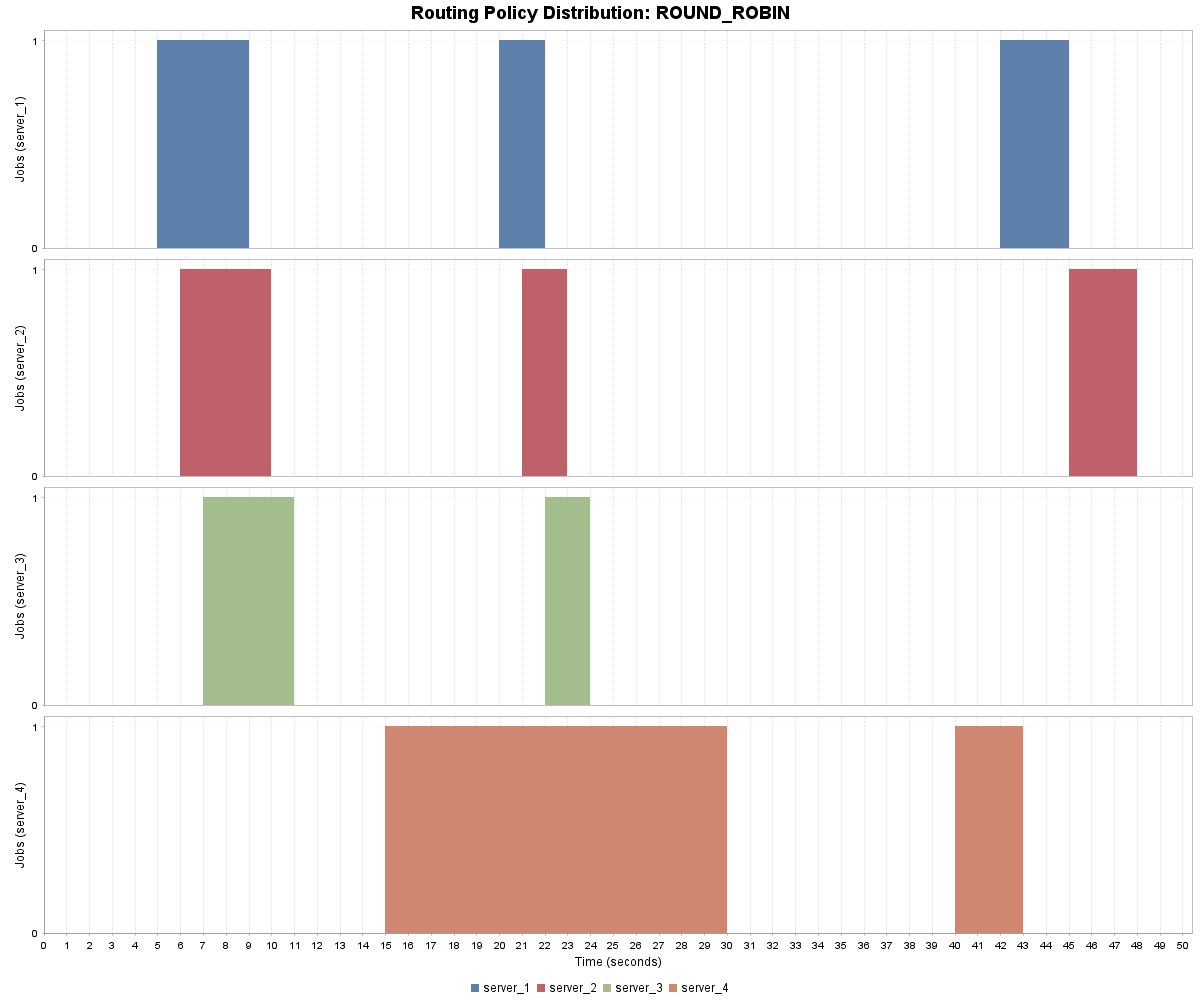
\includegraphics[width=0.64\textwidth]{../data/vv/chart/routing/round_robin.png}
    \caption{Distribuzione temporale dei job sotto politica Round Robin.}
    \label{fig:rr_chart}
\end{figure}

\begin{figure}[H]
    \centering
    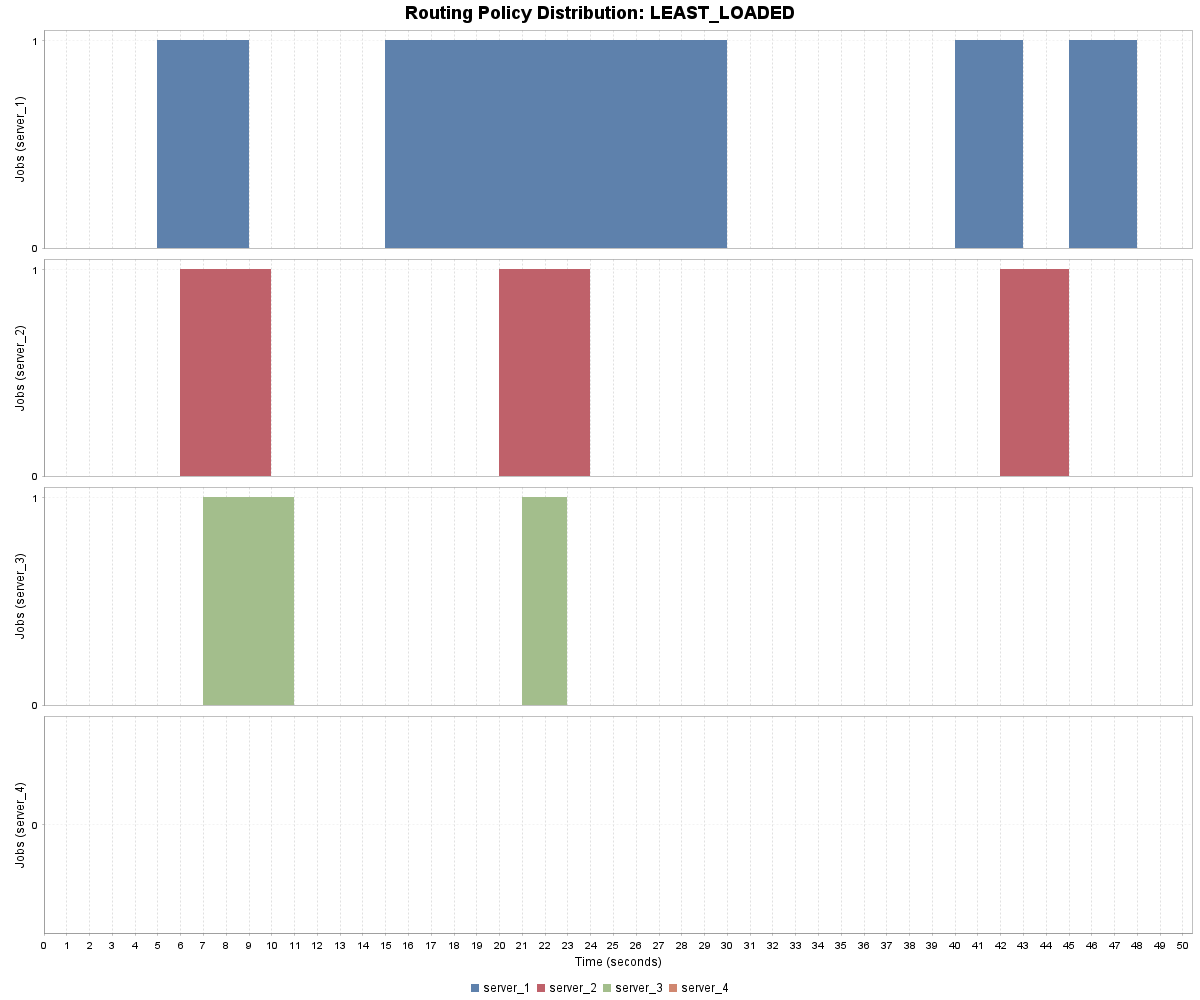
\includegraphics[width=0.64\textwidth]{../data/vv/chart/routing/least_loaded.png}
    \caption{Saturazione dei server sotto politica Least Loaded.}
    \label{fig:ll_chart}
\end{figure}

\begin{figure}[H]
    \centering
    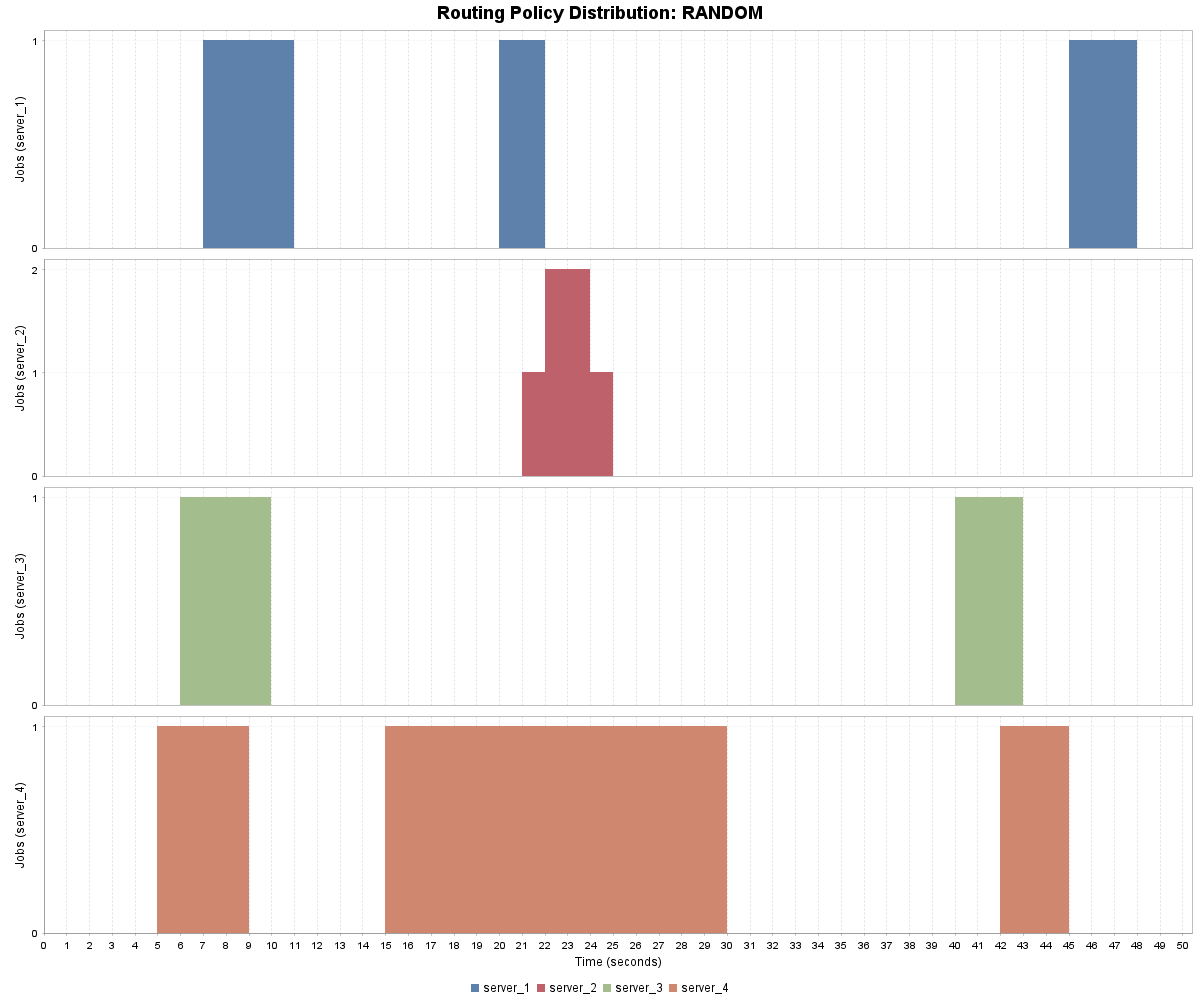
\includegraphics[width=0.64\textwidth]{../data/vv/chart/routing/random.png}
    \caption{Assegnazione stocastica dei task tramite politica Random.}
    \label{fig:rand_chart}
\end{figure}

\begin{figure}[H]
    \centering
    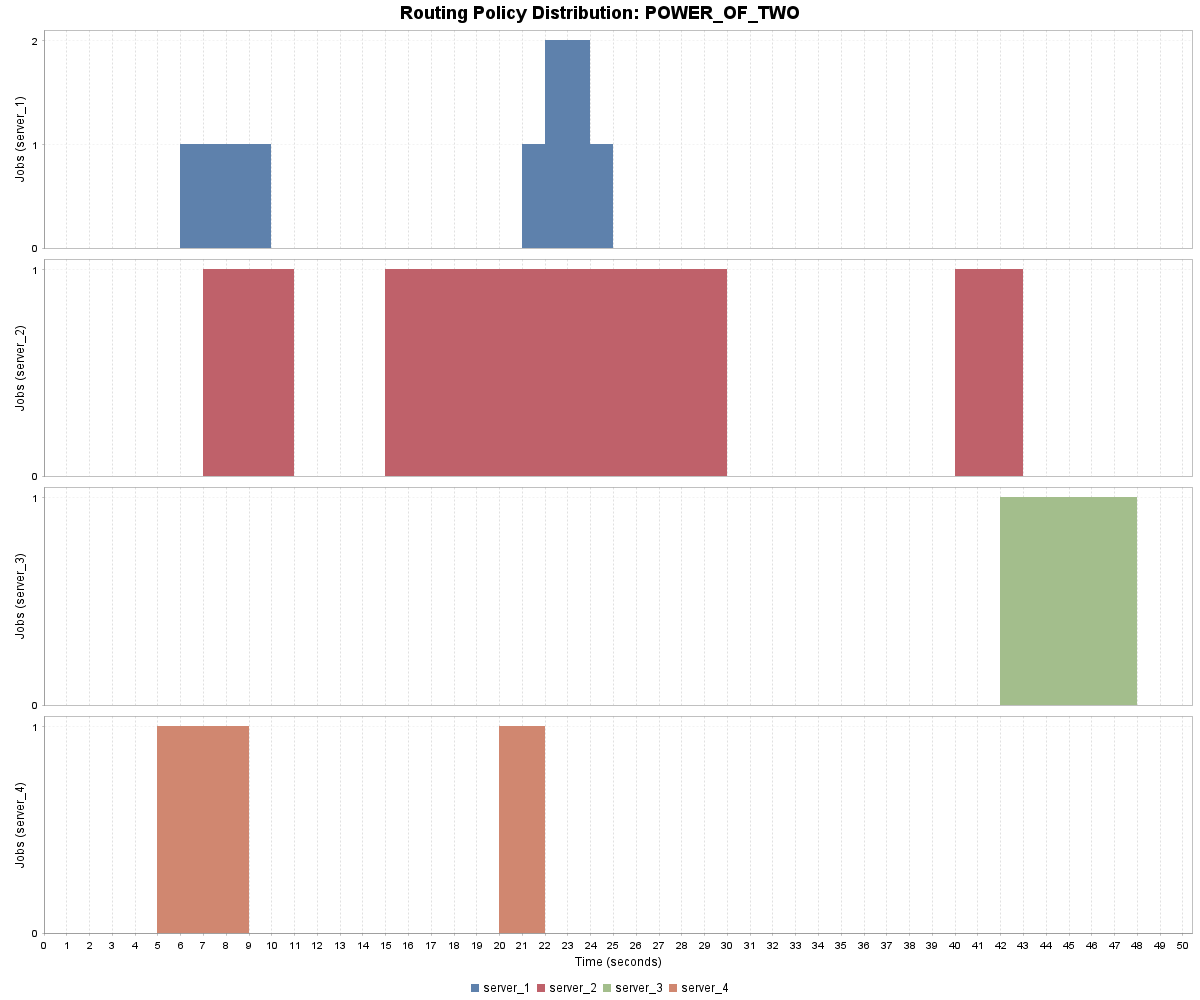
\includegraphics[width=0.64\textwidth]{../data/vv/chart/routing/power_of_two.png}
    \caption{Bilanciamento del carico con tecnica Power of Two Choices.}
    \label{fig:po2_chart}
\end{figure}

\paragraph{Verifica del Meccanismo di Dirottamento verso lo Spike Server:}
Per convalidare la logica di commutazione d'emergenza del router, il modulo è stato sottoposto a uno stress-test deterministico basato su una traccia d'ingresso ad andamento alternato. L'ambiente di verifica viene isolato configurando un cluster minimale composto da un singolo Web Server di linea assistito dallo Spike Server. I parametri operativi del controllore di instradamento sono stati configurati impostando rigidamente la soglia critica a $SI_{max} = 5$ job concorrenti.

% =========================================================================
% LINEA DEL TEMPO DEL CARICO DI LAVORO
% =========================================================================
\begin{figure}[H]
    \centering
    \begin{tikzpicture}[x=0.55cm, y=0.42cm, >=stealth, line width=0.7pt]
        
        % -----------------------------------------------------------------
        % GRIGLIA DI SFONDO
        % -----------------------------------------------------------------
        \foreach \x in {0,2,...,26} {
            \draw[gray!20, dashed] (\x, 0) -- (\x, 22.5);
            \node[below, font=\tiny\sffamily, text=gray!50] at (\x, 0) {\x s};
        }
        
        % Asse temporale principale
        \draw[->, thick, gray!70] (0,0) -- (27.5,0) node[right, font=\small\sffamily\bfseries, text=gray!80] {Tempo};

        % -----------------------------------------------------------------
        % PRIMO BURST COMPLESSO
        % -----------------------------------------------------------------
        \draw[fill=teal!15, draw=teal!80, rounded corners=1pt] (0.0, 1) rectangle (2.0, 1.7);
        \node[right, font=\tiny\sffamily, text=teal!90!black] at (2.0, 1.35) {Job 1 (0.0-2.0s)};
        
        \draw[fill=teal!15, draw=teal!80, rounded corners=1pt] (0.4, 2.2) rectangle (2.4, 2.9);
        \node[right, font=\tiny\sffamily, text=teal!90!black] at (2.4, 2.55) {Job 2 (0.4-2.4s)};
        
        \draw[fill=teal!15, draw=teal!80, rounded corners=1pt] (0.8, 3.4) rectangle (2.8, 4.1);
        \node[right, font=\tiny\sffamily, text=teal!90!black] at (2.8, 3.75) {Job 3 (0.8-2.8s)};
        
        \draw[fill=teal!15, draw=teal!80, rounded corners=1pt] (1.2, 4.6) rectangle (3.2, 5.3);
        \node[right, font=\tiny\sffamily, text=teal!90!black] at (3.2, 4.95) {Job 4 (1.2-3.2s)};
        
        \draw[fill=teal!15, draw=teal!80, rounded corners=1pt] (1.6, 5.8) rectangle (3.6, 6.5);
        \node[right, font=\tiny\sffamily, text=teal!90!black] at (3.6, 6.15) {Job 5 (1.6-3.6s)};
        
        \draw[fill=teal!15, draw=teal!80, rounded corners=1pt] (2.0, 7.0) rectangle (4.0, 7.7);
        \node[right, font=\tiny\sffamily, text=teal!90!black] at (4.0, 7.35) {Job 6 (2.0-4.0s)};
        
        \draw[fill=teal!15, draw=teal!80, rounded corners=1pt] (2.4, 8.2) rectangle (4.4, 8.9);
        \node[right, font=\tiny\sffamily, text=teal!90!black] at (4.4, 8.55) {Job 7 (2.4-4.4s)};
        
        \draw[fill=teal!15, draw=teal!80, rounded corners=1pt] (2.8, 9.4) rectangle (4.8, 10.1);
        \node[right, font=\tiny\sffamily, text=teal!90!black] at (4.8, 9.75) {Job 8 (2.8-4.8s)};
        
        \draw[fill=teal!15, draw=teal!80, rounded corners=1pt] (3.2, 10.6) rectangle (5.2, 11.3);
        \node[right, font=\tiny\sffamily, text=teal!90!black] at (5.2, 10.95) {Job 9 (3.2-5.2s)};
        
        \draw[fill=teal!15, draw=teal!80, rounded corners=1pt] (3.6, 11.8) rectangle (5.6, 12.5);
        \node[right, font=\tiny\sffamily, text=teal!90!black] at (5.6, 12.15) {Job 10 (3.6-5.6s)};
        
        \draw[fill=teal!15, draw=teal!80, rounded corners=1pt] (4.0, 13.0) rectangle (6.0, 13.7);
        \node[right, font=\tiny\sffamily, text=teal!90!black] at (6.0, 13.35) {Job 11 (4.0-6.0s)};
        
        \draw[fill=teal!15, draw=teal!80, rounded corners=1pt] (4.4, 14.2) rectangle (6.4, 14.9);
        \node[right, font=\tiny\sffamily, text=teal!90!black] at (6.4, 14.55) {Job 12 (4.4-6.4s)};

        % -----------------------------------------------------------------
        % JOB ISOLATO
        % -----------------------------------------------------------------
        \draw[fill=orange!15, draw=orange!80, rounded corners=1pt] (8.0, 15.4) rectangle (8.5, 16.1);
        \node[right, font=\tiny\sffamily, text=orange!90!black] at (8.5, 15.75) {Job 13 (8.0-8.5s)};

        % -----------------------------------------------------------------
        % SECONDO BURST
        % -----------------------------------------------------------------
        \draw[fill=cyan!15, draw=cyan!80, rounded corners=1pt] (20.0, 16.6) rectangle (21.0, 17.3);
        \node[right, font=\tiny\sffamily, text=cyan!90!black] at (21.0, 16.95) {Job 14 (20.0-21.0s)};
        
        \draw[fill=cyan!15, draw=cyan!80, rounded corners=1pt] (20.6, 17.8) rectangle (21.6, 18.5);
        \node[right, font=\tiny\sffamily, text=cyan!90!black] at (21.6, 18.15) {Job 15 (20.6-21.6s)};
        
        \draw[fill=cyan!15, draw=cyan!80, rounded corners=1pt] (21.2, 19.0) rectangle (22.2, 19.7);
        \node[right, font=\tiny\sffamily, text=cyan!90!black] at (22.2, 19.35) {Job 16 (21.2-22.2s)};
        
        \draw[fill=cyan!15, draw=cyan!80, rounded corners=1pt] (21.8, 20.2) rectangle (22.8, 20.9);
        \node[right, font=\tiny\sffamily, text=cyan!90!black] at (22.8, 20.55) {Job 17 (21.8-22.8s)};
        
        \draw[fill=cyan!15, draw=cyan!80, rounded corners=1pt] (22.4, 21.4) rectangle (23.4, 22.1);
        \node[right, font=\tiny\sffamily, text=cyan!90!black] at (23.4, 21.75) {Job 18 (22.4-23.4s)};
        
        \draw[fill=cyan!15, draw=cyan!80, rounded corners=1pt] (23.0, 22.6) rectangle (24.0, 23.3);
        \node[right, font=\tiny\sffamily, text=cyan!90!black] at (24.0, 22.95) {Job 19 (23.0-24.0s)};
        
        \draw[fill=cyan!15, draw=cyan!80, rounded corners=1pt] (23.6, 23.8) rectangle (24.6, 24.5);
        \node[right, font=\tiny\sffamily, text=cyan!90!black] at (24.6, 24.15) {Job 20 (23.6-24.6s)};
        
        \draw[fill=cyan!15, draw=cyan!80, rounded corners=1pt] (24.2, 25.0) rectangle (25.2, 25.7);
        \node[right, font=\tiny\sffamily, text=cyan!90!black] at (25.2, 25.35) {Job 21 (24.2-25.2s)};

    \end{tikzpicture}
    \caption{Rappresentazione temporale della traccia stocastica a dente di sega per la verifica del dirottamento sullo Spike Server.}
    \label{fig:spike_trace_timeline}
\end{figure}

L'andamento della dinamica dei flussi, catturato dettagliatamente nella Figura~\ref{fig:spike_load_dynamics}, evidenzia la correttezza matematica delle transizioni di stato del controllore:

\begin{itemize}
    \item \textbf{Fase Ordinaria:} Nella finestra temporale iniziale con $t \in [0, 1.6]\text{ s}$, l'intera massa dei job in ingresso viene assorbita dal Web Server di linea, il cui contatore interno cresce linearmente ad ogni arrivo.
    \item \textbf{Innesco dello Spike Mode:} All'istante esatto in cui il carico locale tocca il valore limite di 5 job concorrenti, il router scatta istantaneamente in modalità di dirottamento. Come visibile dall'emergere dell'area rosa nel grafico, tutti i successivi job del burst vengono veicolati sulla coda dello Spike Server, congelando l'accumulo sul server principale e forzando l'elaborazione distribuita.
    \item \textbf{Rilascio e Svuotamento:} Al cessare del transitorio di picco, lo Spike Server smaltisce i job dirottati operando al massimo delle proprie capacità stazionarie.
\end{itemize}

I report analitici estratti a completamento della run documentano che, a fronte di un tempo di risposta medio globale di 6.9368 secondi e un carico di sistema pari a 5.3953 job, il modulo ha deviato con precisione chirurgica un totale di esattamente 8.0000 job verso l'unità ausiliaria. Questo sversamento controllato ha determinato un'utilizzazione finale dello Spike Server pari esattamente a 0.5000, confermando la perfetta implementazione del ciclo di dirottamento e l'immunità del codice da blocchi o perdite di task durante le transizioni di instradamento. Il risultato è conforme al comportamento atteso: il percorso ausiliario resta inattivo finché il Web Server non raggiunge la soglia, entra in funzione solo per il traffico eccedente e si svuota senza interrompere i job già assegnati.

\begin{figure}[htbp]
    \centering
    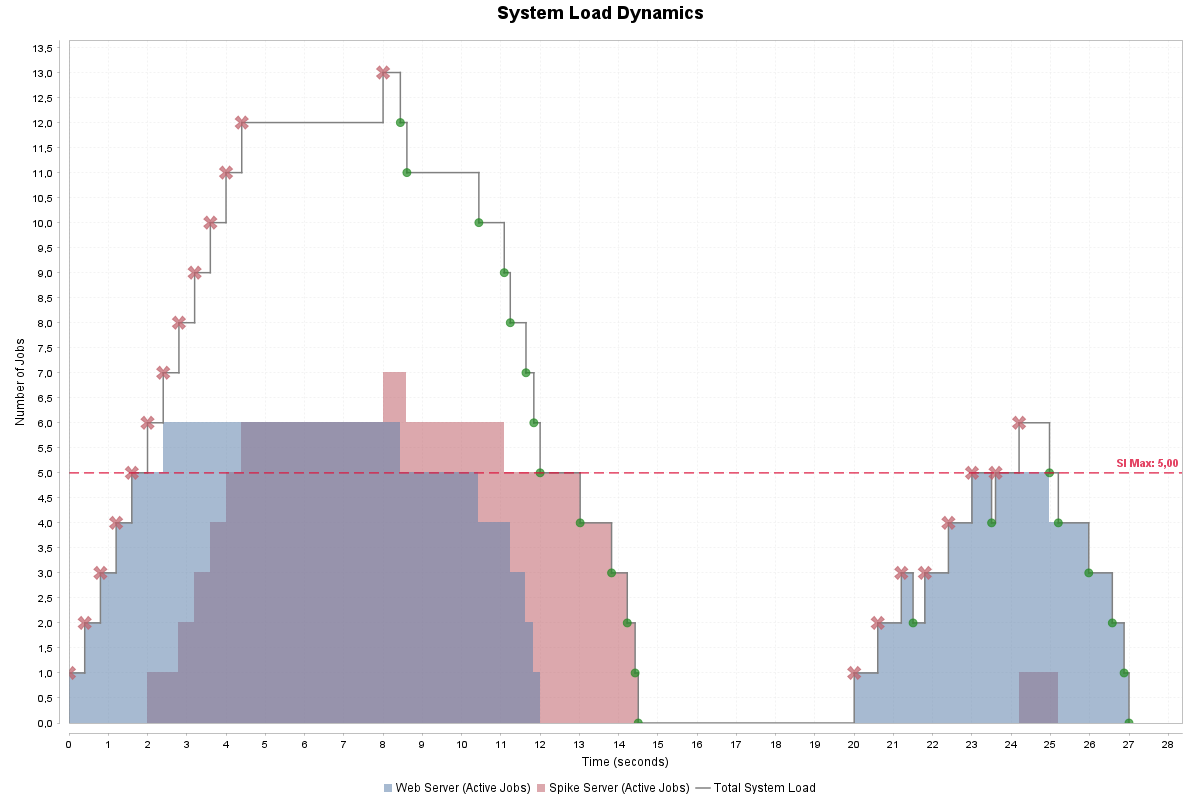
\includegraphics[width=0.9\textwidth]{../data/vv/chart/spike_diversion_chart.png}
    \caption{Evoluzione dinamica del carico e attivazione della Dedicated Spike Unit al superamento della soglia SI Max.}
    \label{fig:spike_load_dynamics}
\end{figure}


\subsection{Verifica dei Meccanismi di Scaling}
L'ultima fase del processo di verifica ha riguardato la verifica funzionale delle logiche di autoscaling cooperativo, accertando la capacità del sistema di espandere o contrarre dinamicamente la propria capacità elaborativa al variare del carico di lavoro imposto.

Anche in questo caso l'esperimento è stato costruito in forma deterministica: l'obiettivo è verificare che le azioni di \textit{Scale Out}, \textit{Scale In}, \textit{Speed Up} e \textit{Speed Down} vengano generate solo quando le metriche finestrate attraversano le rispettive soglie e nel rispetto del \textit{Cooldown}. Il risultato atteso è quindi una corrispondenza puntuale tra istanti di superamento soglia, azioni registrate nei log e andamento dei grafici temporali.

\paragraph{Scaling Orizzontale:}
Per verificare l'adattamento del numero di server attivi guidato dal tempo di risposta, il simulatore è stato configurato con una capacità minima di 1 nodo, un tetto massimo di 4 nodi e un tempo di \textit{Cooldown} di 4.0 secondi. La suite ha eseguito una sottomissione alimentata dalla seguente traccia deterministica programmata di 14 job complessivi (Figura~\ref{fig:horizontal_scaling_trace_timeline}).

% =========================================================================
% LINEA DEL TEMPO DEL CARICO DI LAVORO
% =========================================================================
\begin{figure}[htbp]
    \centering
    \begin{tikzpicture}[x=0.35cm, y=0.45cm, >=stealth, line width=0.7pt]
        
        % -----------------------------------------------------------------
        % GRIGLIA DI SFONDO
        % -----------------------------------------------------------------
        \foreach \x in {0,5,...,40} {
            \draw[gray!20, dashed] (\x, 0) -- (\x, 18.5);
            \node[below, font=\tiny\sffamily, text=gray!50] at (\x, 0) {\x s};
        }
        
        % Asse temporale principale
        \draw[->, thick, gray!70] (0,0) -- (42,0) node[right, font=\small\sffamily\bfseries, text=gray!80] {Tempo};

        % -----------------------------------------------------------------
        % BURST INIZIALE
        % -----------------------------------------------------------------
        \draw[fill=teal!15, draw=teal!80, rounded corners=1pt] (0.0, 1) rectangle (2.0, 1.7);
        \node[right, font=\tiny\sffamily, text=teal!90!black] at (2.0, 1.35) {Job 1 (0.0-2.0s)};
        
        \draw[fill=teal!15, draw=teal!80, rounded corners=1pt] (1.0, 2.2) rectangle (2.5, 2.9);
        \node[right, font=\tiny\sffamily, text=teal!90!black] at (2.5, 2.55) {Job 2 (1.0-2.5s)};
        
        \draw[fill=teal!15, draw=teal!80, rounded corners=1pt] (1.5, 3.4) rectangle (2.5, 4.1);
        \node[right, font=\tiny\sffamily, text=teal!90!black] at (2.5, 3.75) {Job 3 (1.5-2.5s)};
        
        \draw[fill=teal!15, draw=teal!80, rounded corners=1pt] (2.0, 4.6) rectangle (2.5, 5.3);
        \node[right, font=\tiny\sffamily, text=teal!90!black] at (2.5, 4.95) {Job 4 (2.0-2.5s)};

        % -----------------------------------------------------------------
        % SECONDO IMPULSO
        % -----------------------------------------------------------------
        \draw[fill=orange!15, draw=orange!80, rounded corners=1pt] (11.0, 5.8) rectangle (13.5, 6.5);
        \node[right, font=\tiny\sffamily, text=orange!90!black] at (13.5, 6.15) {Job 5 (11.0-13.5s)};
        
        \draw[fill=orange!15, draw=orange!80, rounded corners=1pt] (11.0, 7.0) rectangle (13.5, 7.7);
        \node[right, font=\tiny\sffamily, text=orange!90!black] at (13.5, 7.35) {Job 6 (11.0-13.5s)};

        % -----------------------------------------------------------------
        % TERZO BURST RAPIDO
        % -----------------------------------------------------------------
        \draw[fill=cyan!15, draw=cyan!80, rounded corners=1pt] (15.0, 8.2) rectangle (15.2, 8.9);
        \node[right, font=\tiny\sffamily, text=cyan!90!black] at (15.2, 8.55) {Job 7 (15.0-15.2s)};
        
        \draw[fill=cyan!15, draw=cyan!80, rounded corners=1pt] (15.0, 9.4) rectangle (15.2, 10.1);
        \node[right, font=\tiny\sffamily, text=cyan!90!black] at (15.2, 9.75) {Job 8 (15.0-15.2s)};
        
        \draw[fill=cyan!15, draw=cyan!80, rounded corners=1pt] (15.0, 10.6) rectangle (15.2, 11.3);
        \node[right, font=\tiny\sffamily, text=cyan!90!black] at (15.2, 10.95) {Job 9 (15.0-15.2s)};

        % -----------------------------------------------------------------
        % QUARTO IMPULSO
        % -----------------------------------------------------------------
        \draw[fill=olive!15, draw=olive!80, rounded corners=1pt] (25.0, 11.8) rectangle (25.5, 12.5);
        \node[right, font=\tiny\sffamily, text=olive!90!black] at (25.5, 12.15) {Job 10 (25.0-25.5s)};
        
        \draw[fill=olive!15, draw=olive!80, rounded corners=1pt] (25.0, 13.0) rectangle (25.5, 13.7);
        \node[right, font=\tiny\sffamily, text=olive!90!black] at (25.5, 13.35) {Job 11 (25.0-25.5s)};

        % -----------------------------------------------------------------
        % QUINTO BURST FINALE
        % -----------------------------------------------------------------
        \draw[fill=violet!15, draw=violet!80, rounded corners=1pt] (35.0, 14.2) rectangle (37.0, 14.9);
        \node[right, font=\tiny\sffamily, text=violet!90!black] at (37.0, 14.55) {Job 12 (35.0-37.0s)};
        
        \draw[fill=violet!15, draw=violet!80, rounded corners=1pt] (35.0, 15.4) rectangle (37.0, 16.1);
        \node[right, font=\tiny\sffamily, text=violet!90!black] at (37.0, 15.75) {Job 13 (35.0-37.0s)};
        
        \draw[fill=violet!15, draw=violet!80, rounded corners=1pt] (35.0, 16.6) rectangle (37.0, 17.3);
        \node[right, font=\tiny\sffamily, text=violet!90!black] at (37.0, 16.95) {Job 14 (35.0-37.0s)};

    \end{tikzpicture}
    \caption{Rappresentazione temporale della traccia deterministica dei job in ingresso per la verifica del modulo di Scaling Orizzontale.}
    \label{fig:horizontal_scaling_trace_timeline}
\end{figure}

Le soglie di attuazione dell'algoritmo di controllo sono state impostate a $T_{out} = 2.0\text{ s}$ per l'innesco dello \textit{Scale Out} e a $T_{in} = 0.5\text{ s}$ per lo \textit{Scale In}. 

L'analisi dell'andamento temporale documentato nella Figura~\ref{fig:horizontal_scaling_dynamics} convalida formalmente l'esattezza algoritmica del modulo:
\begin{itemize}
    \item \textbf{Dinamica di Scale Out:} Al secondo $t = 4.0$, l'accumulo di job porta il tempo medio di risposta nella Moving Window a superare la soglia critica di $2.0\text{ s}$ (toccando quota $2.15\text{ s}$). Il sistema reagisce istantaneamente incrementando i server attivi da 1 a 2 e avviando il timer di \textit{Cooldown} di $4.0\text{ s}$. Poiché il carico permane elevato, alla scadenza di ciascun ciclo di blocco si osservano i successivi scatti incrementali a quota 3 server (al secondo $t = 8.0$) e a quota 4 server (al secondo $t = 13.5$), azzerando la saturazione. Un'ultima azione isolata di espansione a 3 server si ripresenta correttamente al secondo $t = 39.0$ per mitigare l'ultimo burst, totalizzando l'esatto valore nominale di 4 azioni di \textit{Scale Out} registrato nei log di report.
    \item \textbf{Dinamica di Scale In e Draining:} Al secondo $t = 15.0$, l'immissione di job molto rapidi abbatte drasticamente il tempo medio di risposta sotto la soglia di $0.5\text{ s}$. Non appena il \textit{Cooldown} residuo si azzera, l'analizzatore comanda una contrazione della flotta, riducendo i server da 4 a 3 (all'istante $t = 25.5$) e successivamente da 3 a 2 (all'istante $t = 29.5$), quantificando le 2 azioni di \textit{Scale In} complessive presenti nel riepilogo statistico. La correttezza del meccanismo di \textit{draining} trova riscontro diretto nell'andamento dei completamenti: il server rimosso cessa l'accettazione di nuovi task ma non interrompe le elaborazioni in corso, azzerando la sua coda interna in modo conservativo senza alcuna perdita di eventi.
\end{itemize}

\begin{figure}[H]
    \centering
    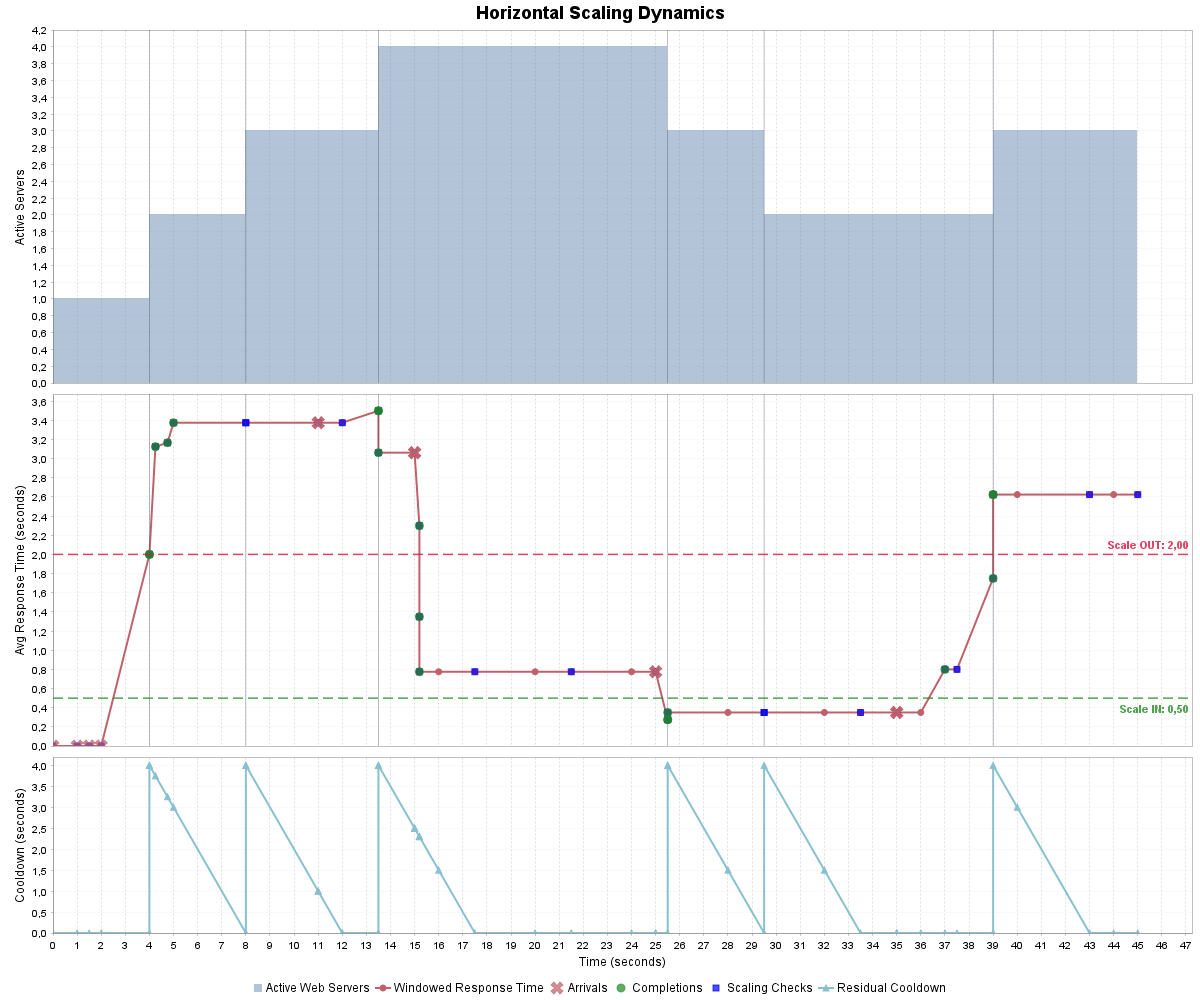
\includegraphics[width=0.85\textwidth]{../data/vv/chart/scaling/horizontal_scaling_chart.png}
    \caption{Evoluzione temporale dello Scaling Orizzontale: correlazione tra tempo di risposta finestrato, azioni di allocazione e vincolo di Cooldown.}
    \label{fig:horizontal_scaling_dynamics}
\end{figure}

\paragraph{Scaling Verticale:}
La validazione delle logiche di allocazione delle risorse hardware si è concentrata sulla riconfigurazione dinamica della capacità di calcolo dello Spike Server. In questo scenario, il sistema opera su un singolo server di linea e dirotta i job in eccesso sull'unità di picco ausiliaria. Le soglie di reazione per la modulazione della frequenza core sono state configurate a un valore limite superiore di 3 job concorrenti in coda e a una soglia inferiore di 1 job per il ripristino ordinario. Il timer di \textit{Cooldown} interno del regolatore è stato ridotto a $0.3$ secondi per garantire reattività immediata. La traccia di stress-test iniettata nel sistema prevede due flussi programmati distinti (mostrati in Figura~\ref{fig:vertical_scaling_trace_timeline}).

% =========================================================================
% LINEA DEL TEMPO DEL CARICO DI LAVORO
% =========================================================================
\begin{figure}[htbp]
    \centering
    \begin{tikzpicture}[x=0.55cm, y=0.45cm, >=stealth, line width=0.7pt]
        
        % -----------------------------------------------------------------
        % GRIGLIA DI SFONDO
        % -----------------------------------------------------------------
        \foreach \x in {0,2,...,26} {
            \draw[gray!20, dashed] (\x, 0) -- (\x, 15.5);
            \node[below, font=\tiny\sffamily, text=gray!50] at (\x, 0) {\x s};
        }
        
        % Asse temporale principale
        \draw[->, thick, gray!70] (0,0) -- (27.5,0) node[right, font=\small\sffamily\bfseries, text=gray!80] {Tempo};

        % -----------------------------------------------------------------
        % BURST DI PICCO INIZIALE
        % -----------------------------------------------------------------
        \draw[fill=orange!15, draw=orange!80, rounded corners=1pt] (1.0, 1) rectangle (5.0, 1.7);
        \node[right, font=\tiny\sffamily, text=orange!90!black] at (5.0, 1.35) {Job 1 (1.0-5.0s)};
        
        \draw[fill=orange!15, draw=orange!80, rounded corners=1pt] (1.3, 2.2) rectangle (5.3, 2.9);
        \node[right, font=\tiny\sffamily, text=orange!90!black] at (5.3, 2.55) {Job 2 (1.3-5.3s)};
        
        \draw[fill=orange!15, draw=orange!80, rounded corners=1pt] (1.6, 3.4) rectangle (5.6, 4.1);
        \node[right, font=\tiny\sffamily, text=orange!90!black] at (5.6, 3.75) {Job 3 (1.6-5.6s)};
        
        \draw[fill=orange!15, draw=orange!80, rounded corners=1pt] (1.9, 4.6) rectangle (5.9, 5.3);
        \node[right, font=\tiny\sffamily, text=orange!90!black] at (5.9, 4.95) {Job 4 (1.9-5.9s)};
        
        \draw[fill=orange!15, draw=orange!80, rounded corners=1pt] (2.2, 5.8) rectangle (6.2, 6.5);
        \node[right, font=\tiny\sffamily, text=orange!90!black] at (6.2, 6.15) {Job 5 (2.2-6.2s)};
        
        \draw[fill=orange!15, draw=orange!80, rounded corners=1pt] (2.5, 7.0) rectangle (6.5, 7.7);
        \node[right, font=\tiny\sffamily, text=orange!90!black] at (6.5, 7.35) {Job 6 (2.5-6.5s)};
        
        \draw[fill=orange!15, draw=orange!80, rounded corners=1pt] (2.8, 8.2) rectangle (6.8, 8.9);
        \node[right, font=\tiny\sffamily, text=orange!90!black] at (6.8, 8.55) {Job 7 (2.8-6.8s)};

        % -----------------------------------------------------------------
        % FASE POST-PICCO DI RILASCIO
        % -----------------------------------------------------------------
        \draw[fill=teal!15, draw=teal!80, rounded corners=1pt] (12.0, 9.4) rectangle (12.5, 10.1);
        \node[right, font=\tiny\sffamily, text=teal!90!black] at (12.5, 9.75) {Job 8 (12.0-12.5s)};
        
        \draw[fill=teal!15, draw=teal!80, rounded corners=1pt] (15.0, 10.6) rectangle (15.5, 11.3);
        \node[right, font=\tiny\sffamily, text=teal!90!black] at (15.5, 10.95) {Job 9 (15.0-15.5s)};
        
        \draw[fill=teal!15, draw=teal!80, rounded corners=1pt] (18.0, 11.8) rectangle (18.5, 12.5);
        \node[right, font=\tiny\sffamily, text=teal!90!black] at (18.5, 12.15) {Job 10 (18.0-18.5s)};
        
        \draw[fill=teal!15, draw=teal!80, rounded corners=1pt] (21.0, 13.0) rectangle (21.5, 13.7);
        \node[right, font=\tiny\sffamily, text=teal!90!black] at (21.5, 13.35) {Job 11 (21.0-21.5s)};
        
        \draw[fill=teal!15, draw=teal!80, rounded corners=1pt] (24.0, 14.2) rectangle (24.5, 14.9);
        \node[right, font=\tiny\sffamily, text=teal!90!black] at (24.5, 14.55) {Job 12 (24.0-24.5s)};

    \end{tikzpicture}
    \caption{Rappresentazione temporale della traccia deterministica dei job in ingresso per la verifica del modulo di Scaling Verticale.}
    \label{fig:vertical_scaling_trace_timeline}
\end{figure}

I risultati della simulazione, illustrati graficamente nella Figura~\ref{fig:vertical_scaling_dynamics}, dimostrano una perfetta coincidenza tra il comportamento atteso e le transizioni osservate. Al secondo $t = 2.0$, il cumulo di task all'interno dello Spike Server supera la soglia critica di 3 job attivi. Il controllore verticale interviene senza ritardi temporali registrando 1 azione di \textit{Speed Up}, la quale innalza istantaneamente il moltiplicatore di velocità dell'infrastruttura dal valore base di 4.0 a un livello di picco pari a 8.0. Grazie a questa accelerazione controllata, la coda viene smaltita rapidamente: al secondo $t = 4.4$, il numero di job residenti scende sotto la soglia minima di 1. Il software applica quindi l'esatta transizione duale di \textit{Speed Down}, riportando il moltiplicatore alla frequenza nominale di 4.0. 

Il perfetto confinamento di queste transizioni all'interno della finestra di massimo carico giustifica il valore del moltiplicatore di velocità medio complessivo registrato nel report finale, attestatosi a 4.3840. Il bilancio di fine simulazione conferma l'esecuzione di esattamente 1 azione di Speed Up e 1 azione di Speed Down, validando la totale assenza di fenomeni di instabilità o derive computazionali nelle routine di controllo verticale.

\begin{figure}[H]
    \centering
    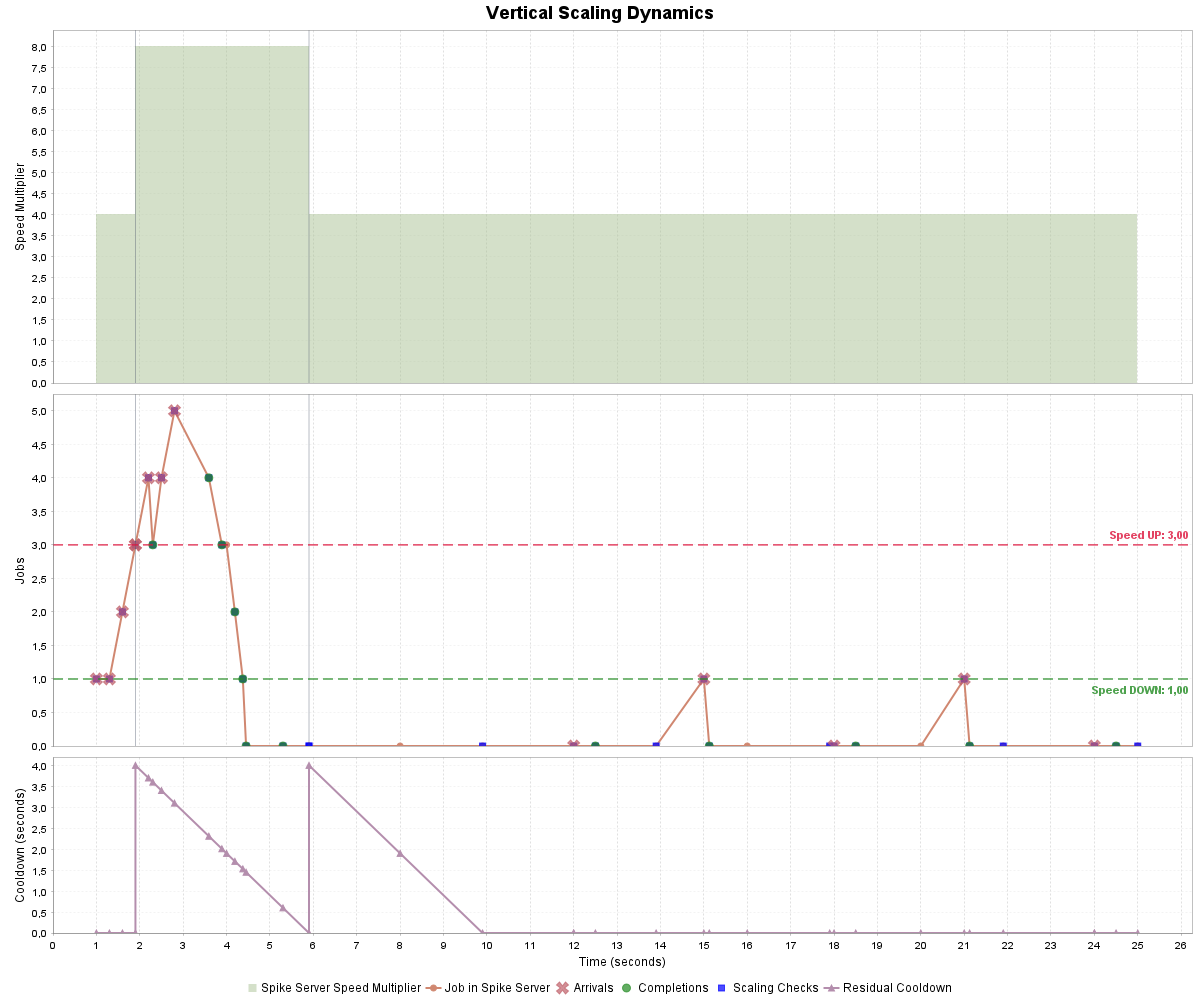
\includegraphics[width=0.85\textwidth]{../data/vv/chart/scaling/vertical_scaling_chart.png}
    \caption{Dinamica dello Scaling Verticale: modulazione istantanea del moltiplicatore di velocità in funzione del numero di job residenti nella coda dello Spike Server.}
    \label{fig:vertical_scaling_dynamics}
\end{figure}

\clearpage


% =========================================================================
% VALIDAZIONE
% =========================================================================
\section{Validazione del Sistema}
La validazione rappresenta il passaggio successivo alla verifica: non si limita ad accertare che il codice implementi correttamente le transizioni previste dal modello, ma controlla che le misure prodotte dal simulatore siano compatibili con quelle ottenute da un ambiente di riferimento indipendente. Per questo motivo i risultati principali sono stati confrontati con il simulatore fornito dal libro di testo, ovvero \textit{Java Modelling Tools - JSIM} \cite{jmt-software}, riproducendo gli stessi scenari di carico, la stessa disciplina di servizio e le stesse ipotesi di assenza di autoscaling.

La validazione è stata condotta in orizzonte infinito, con misure stazionarie e intervalli di confidenza sulle metriche aggregate. Nel simulatore sviluppato, le stime sono state ottenute con il metodo dei \textit{Batch Means}; in JSIM sono state invece usate le misure statistiche native del tool, configurate con seed fisso e criterio di arresto basato sul numero massimo di campioni analizzati. L'obiettivo del confronto non è dunque riprodurre la stessa sequenza di eventi elementari, ma verificare che due implementazioni indipendenti dello stesso sistema convergano agli stessi indici prestazionali entro la variabilità statistica attesa.

Per ciascun caso di validazione è stato quindi definito un comportamento atteso prima dell'esecuzione: sovrapposizione degli intervalli di confidenza per la stazione singola, e scarti contenuti per l'architettura completa, dove JSIM richiede una rappresentazione semplificata del router a soglia. Eventuali differenze residue non vengono interpretate come errore se restano coerenti con le diverse astrazioni modellistiche e con l'ampiezza degli intervalli statistici.

\subsection{Validazione della Stazione Singola Iperesponenziale}
Il primo scenario di validazione isola una singola stazione \textit{Processor Sharing}, eliminando ogni effetto dovuto al routing, allo Spike Server e agli algoritmi di scaling. La rete JSIM di riferimento è composta da una sorgente aperta, una coda a capacità illimitata e un sink finale. Sia gli interarrivi sia i tempi di servizio seguono una distribuzione iperesponenziale a due rami, con tasso medio di arrivo $\lambda = 2.5\text{ job/s}$, tasso medio di servizio $\mu = 4.0\text{ job/s}$ e coefficiente di variazione $C_V = 4.0$.

La parametrizzazione JSIM della distribuzione $H_2$ è stata impostata con probabilità di ramo $p = 0.030776$; per gli interarrivi sono stati usati $\lambda_1 = 0.15388$ e $\lambda_2 = 4.84612$, mentre per i servizi $\lambda_1 = 0.24621$ e $\lambda_2 = 7.75379$. Il modello JSIM è stato eseguito con seed $123456789$, stop statistico disabilitato, $100000000$ campioni massimi e intervalli di confidenza al $99\%$ con errore relativo massimo pari a $0.03$. Nel simulatore Java è stata usata una run a Batch Means da $512$ batch di $16384$ job, con warm-up nullo, coerentemente con la configurazione già impiegata nella verifica statistica.

Prima del confronto diretto, la dimensione dei batch è stata stimata tramite l'algoritmo di \textit{Batch Means Estimator}. L'output, riportato in Tabella~\ref{tab:validation_hyperexp_batch}, mostra che il metodo dinamico raggiunge simultaneamente indipendenza e precisione relativa, mentre il metodo basato su ACF produce una struttura più ampia e conservativa.

\begin{table}[htbp]
    \centering
    \small
    \renewcommand{\arraystretch}{1.3}
    \begin{tabular}{lccccc}
        \hline
        \textbf{Metodo} & \textbf{Dim. Batch} & \textbf{Num. Batch} & \textbf{Lag-1 ACF} & \textbf{Media Stimata} & \textbf{Half-Width} \\ \hline
        ACF             & $11970$             & $417$               & $0.0656$           & $1.1970\text{ s}$      & $0.0197$            \\
        Dinamico        & $65536$             & $32$                & $0.0248$           & $1.1939\text{ s}$      & $0.0419$            \\ \hline
    \end{tabular}
    \caption{Calibrazione del Batch Means Estimator per la validazione del modello $H_2/H_2/1$.}
    \label{tab:validation_hyperexp_batch}
\end{table}

\begin{figure}[H]
    \centering

    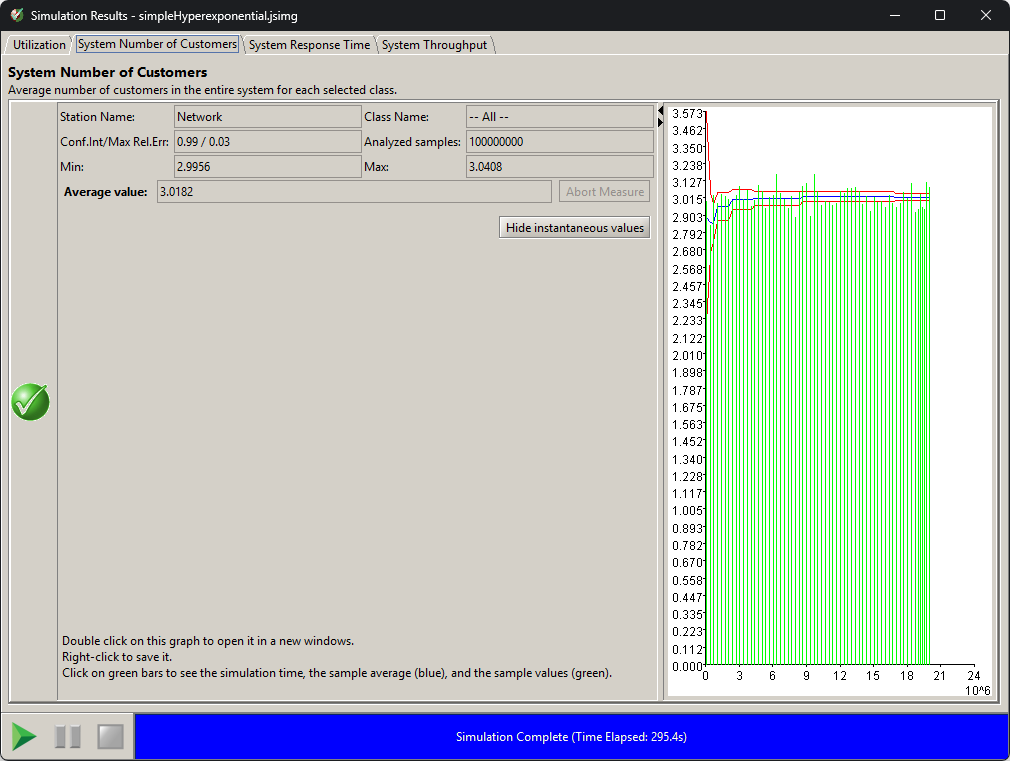
\includegraphics[
        width=0.88\textwidth,
        trim=0 380 0 25,
        clip
    ]{../data/simulation/simple_hyperexp/job}

    \vspace{0.015\textheight}

    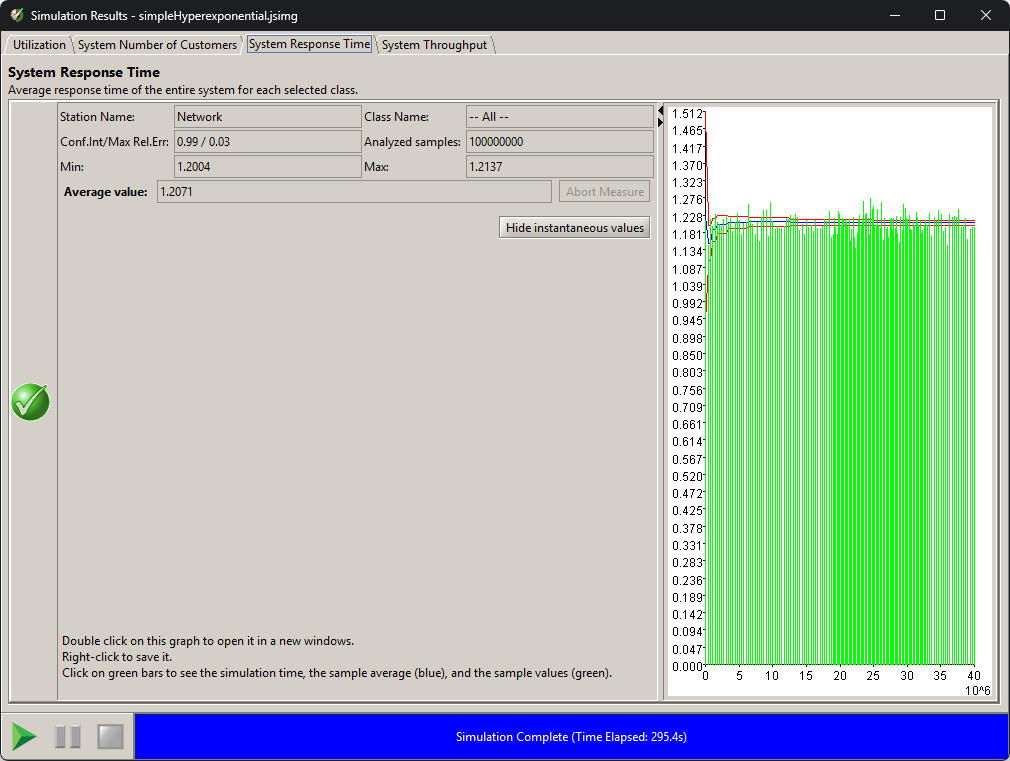
\includegraphics[
        width=0.88\textwidth,
        trim=0 380 0 25,
        clip
    ]{../data/simulation/simple_hyperexp/response}

    \vspace{0.015\textheight}

    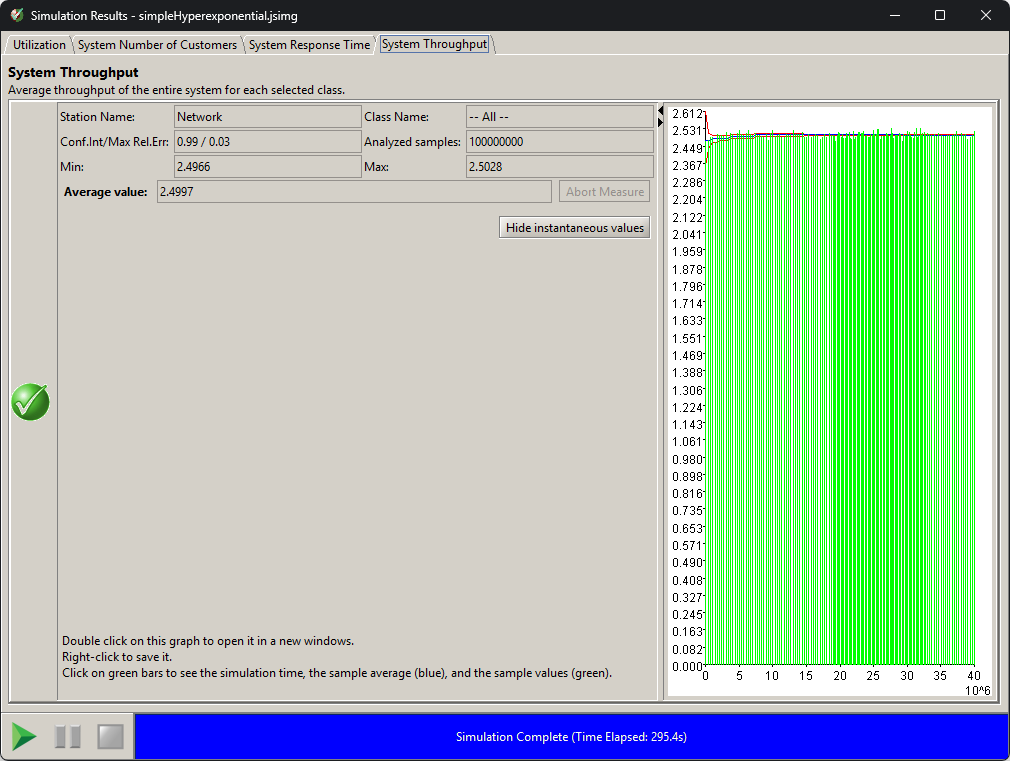
\includegraphics[
        width=0.88\textwidth,
        trim=0 380 0 25,
        clip
    ]{../data/simulation/simple_hyperexp/throughput}

    \vspace{0.015\textheight}

    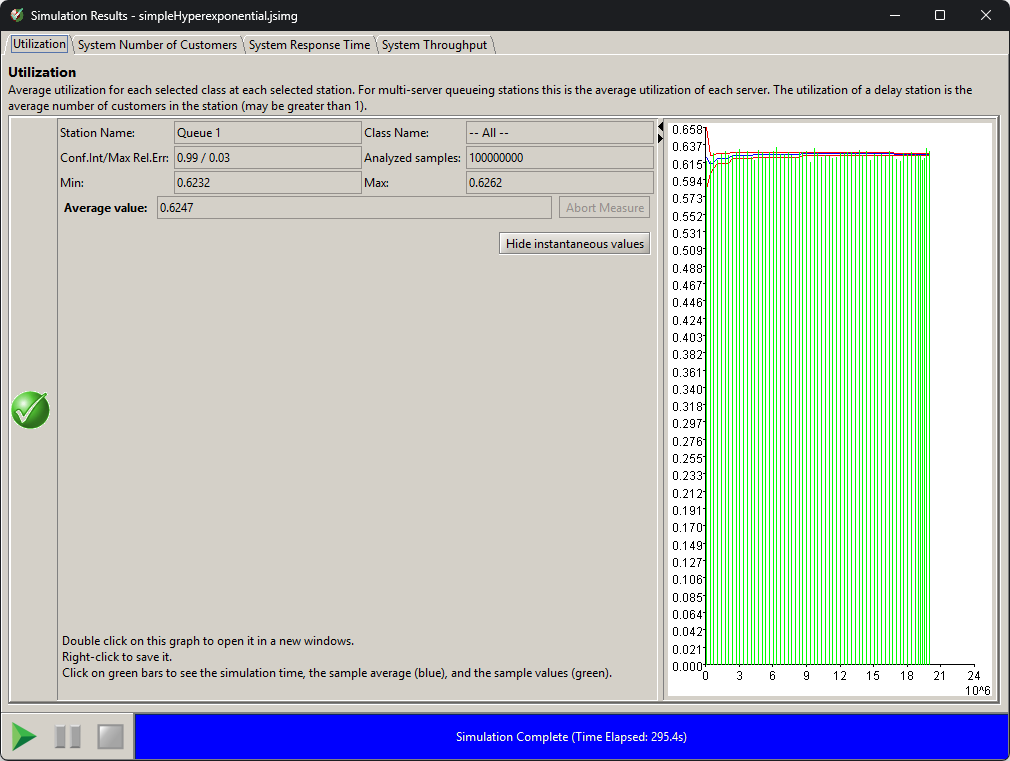
\includegraphics[
        width=0.88\textwidth,
        trim=0 380 0 25,
        clip
    ]{../data/simulation/simple_hyperexp/utilization}

    \caption{Risultati JSIM per la validazione della stazione singola iperesponenziale.}
    \label{fig:jsim_hyperexp_validation}
\end{figure}

Il confronto numerico è riassunto nella Tabella~\ref{tab:validation_hyperexp_comparison}. Il valore atteso, in questo scenario, è una coincidenza quasi diretta delle metriche, poiché entrambi i simulatori rappresentano la stessa singola stazione senza logiche di controllo aggiuntive. Le metriche ottenute dai due simulatori risultano infatti sostanzialmente coincidenti: il tempo medio di risposta differisce dello $0.80\%$, il numero medio di job dello $0.67\%$, il throughput dello $0.02\%$ e l'utilizzazione dello $0.11\%$. Inoltre, gli intervalli di confidenza delle due campagne si sovrappongono per tutte le metriche osservate, confermando che la dinamica di servizio, l'integrazione temporale delle aree e il calcolo degli indici a regime sono coerenti con il simulatore di riferimento.

\begin{table}[htbp]
    \centering
    \small
    \renewcommand{\arraystretch}{1.3}
    \begin{tabular}{lcccc}
        \hline
        \textbf{Metrica} & \textbf{Simulatore Java} & \textbf{CI Java 95\%} & \textbf{JSIM} & \textbf{CI JSIM 99\%} \\ \hline
        $E[T_s]$         & $1.1975\text{ s}$        & $[1.1826, 1.2123]$    & $1.2071\text{ s}$ & $[1.2004, 1.2137]$ \\
        $E[N_s]$         & $2.9979$                 & $[2.9561, 3.0398]$    & $3.0182$          & $[2.9956, 3.0408]$ \\
        $X$              & $2.4991\text{ job/s}$    & $[2.4921, 2.5062]$    & $2.4997\text{ job/s}$ & $[2.4966, 2.5028]$ \\
        $\rho$           & $0.6240$                 & $[0.6215, 0.6265]$    & $0.6247$          & $[0.6232, 0.6262]$ \\ \hline
    \end{tabular}
    \caption{Confronto di validazione tra simulatore Java e JSIM sul modello $H_2/H_2/1$.}
    \label{tab:validation_hyperexp_comparison}
\end{table}

\subsection{Validazione dell'Architettura Web Server e Spike Server}
Il secondo scenario estende la validazione alla struttura architetturale composta da un Web Server ordinario e da uno Spike Server di supporto. In questo caso l'obiettivo non è verificare una singola stazione, ma accertare che il meccanismo aggregato di instradamento verso il livello ausiliario produca lo stesso ordine di grandezza prestazionale del modello JSIM di riferimento.

Per isolare il solo comportamento del routing, entrambi gli autoscaler sono stati disabilitati: il numero di Web Server resta costante, il moltiplicatore dello Spike Server non varia nel tempo e non vengono eseguite azioni di \textit{Scale Out}, \textit{Scale In}, \textit{Scale Up} o \textit{Scale Down}. Il traffico in ingresso rimane iperesponenziale, con $\lambda = 2.5\text{ job/s}$ e $C_V = 4.0$; i servizi delle stazioni sono modellati con lo stesso schema $H_2$ e tasso medio $\mu = 4.0\text{ job/s}$. In JSIM il comportamento a soglia del router è stato emulato tramite una rete ausiliaria di token e transizioni: la classe chiusa \textit{maxReq\_Link}, inizializzata con $10$ token nella place \textit{P\_Tokens}, permette di riprodurre il vincolo di capacità del percorso ordinario e di inviare il traffico eccedente verso lo Spike Server.

Questa costruzione rappresenta una semplificazione esplicita rispetto alla \textit{ThresholdSpikeServerRoutingStrategy} implementata nel simulatore Java: JSIM non esegue lo stesso controllo oggetto-per-oggetto sul valore istantaneo di $SI$ del Web Server, ma ne riproduce l'effetto macroscopico mediante abilitazione e inibizione delle transizioni. Il confronto va quindi interpretato come validazione delle metriche globali del sistema a due livelli, non come equivalenza perfetta delle singole decisioni di routing.

Anche per questo scenario è stata eseguita una stima preliminare dei Batch Means sul tempo di risposta globale. La Tabella~\ref{tab:validation_system_batch} mostra che il metodo ACF suggerisce batch da $2360$ job, mentre il metodo dinamico converge con batch da $512$ job dopo avere soddisfatto il vincolo di autocorrelazione e quello di precisione relativa.

\begin{table}[htbp]
    \centering
    \small
    \renewcommand{\arraystretch}{1.3}
    \begin{tabular}{lccccc}
        \hline
        \textbf{Metodo} & \textbf{Dim. Batch} & \textbf{Num. Batch} & \textbf{Lag-1 ACF} & \textbf{Media Stimata} & \textbf{Half-Width} \\ \hline
        ACF             & $2360$              & $2118$              & $0.0628$           & $0.9161\text{ s}$      & $0.0064$            \\
        Dinamico        & $512$               & $195$               & $-0.0406$          & $0.9420\text{ s}$      & $0.0463$            \\ \hline
    \end{tabular}
    \caption{Calibrazione del Batch Means Estimator per la validazione dell'architettura Web Server e Spike Server.}
    \label{tab:validation_system_batch}
\end{table}

\begin{figure}[H]
    \centering

    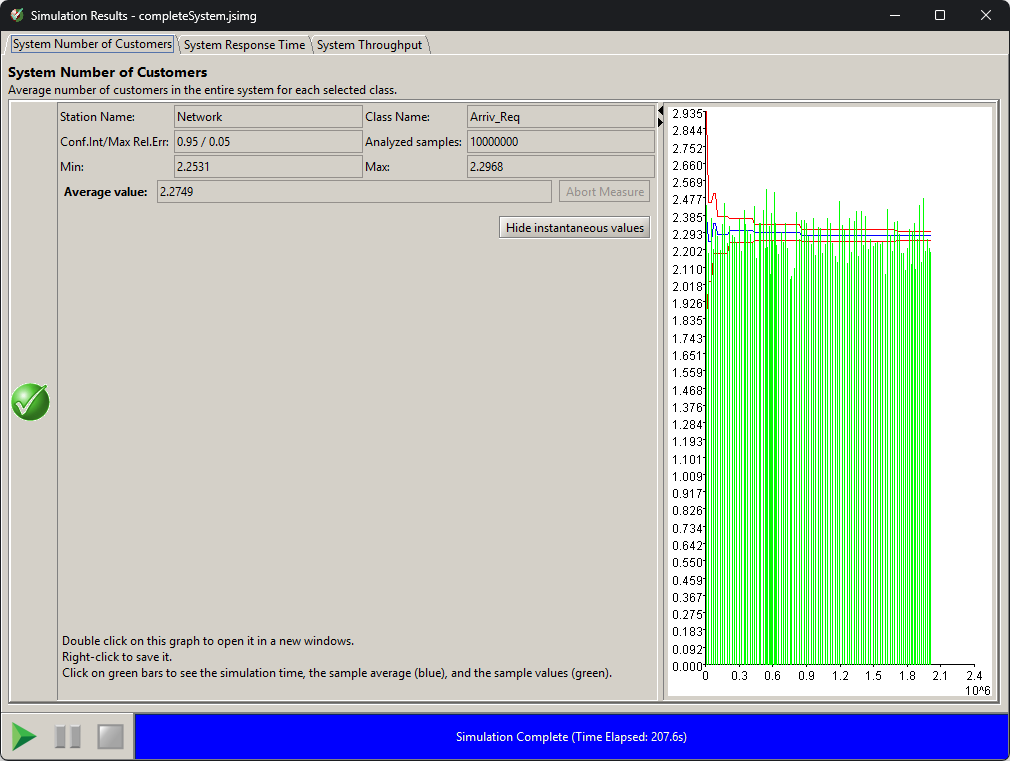
\includegraphics[
        width=0.88\textwidth,
        trim=0 380 0 25,
        clip
    ]{../data/simulation/simple_system/job}

    \vspace{0.02\textheight}

    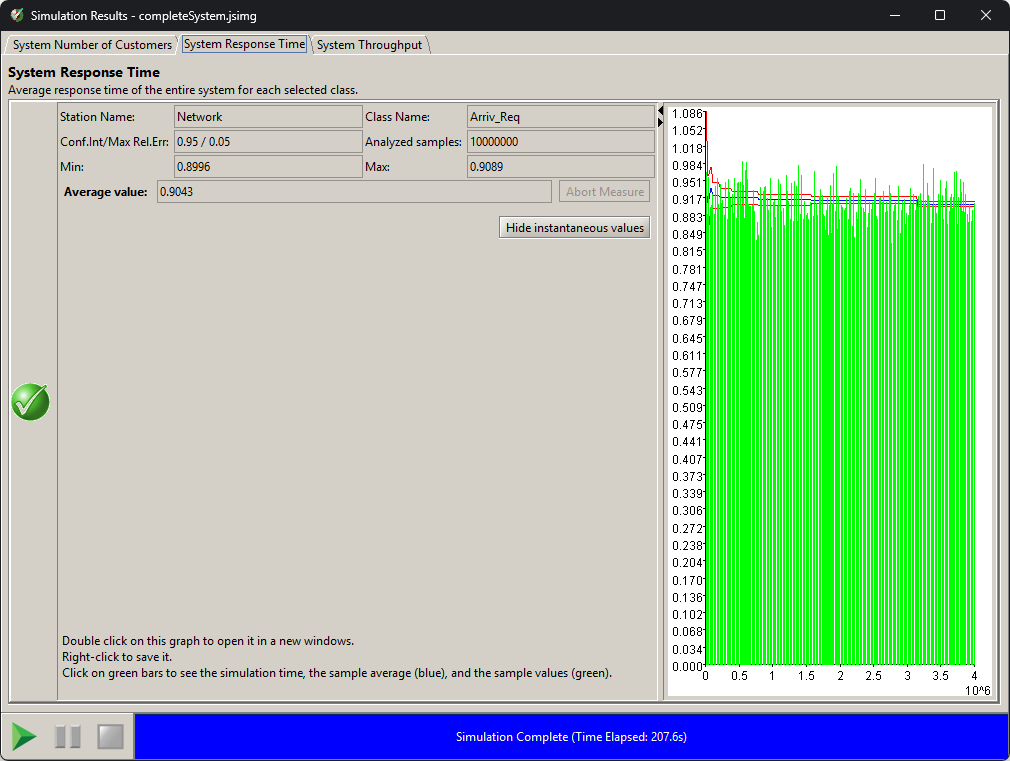
\includegraphics[
        width=0.88\textwidth,
        trim=0 380 0 25,
        clip
    ]{../data/simulation/simple_system/response}

    \vspace{0.02\textheight}

    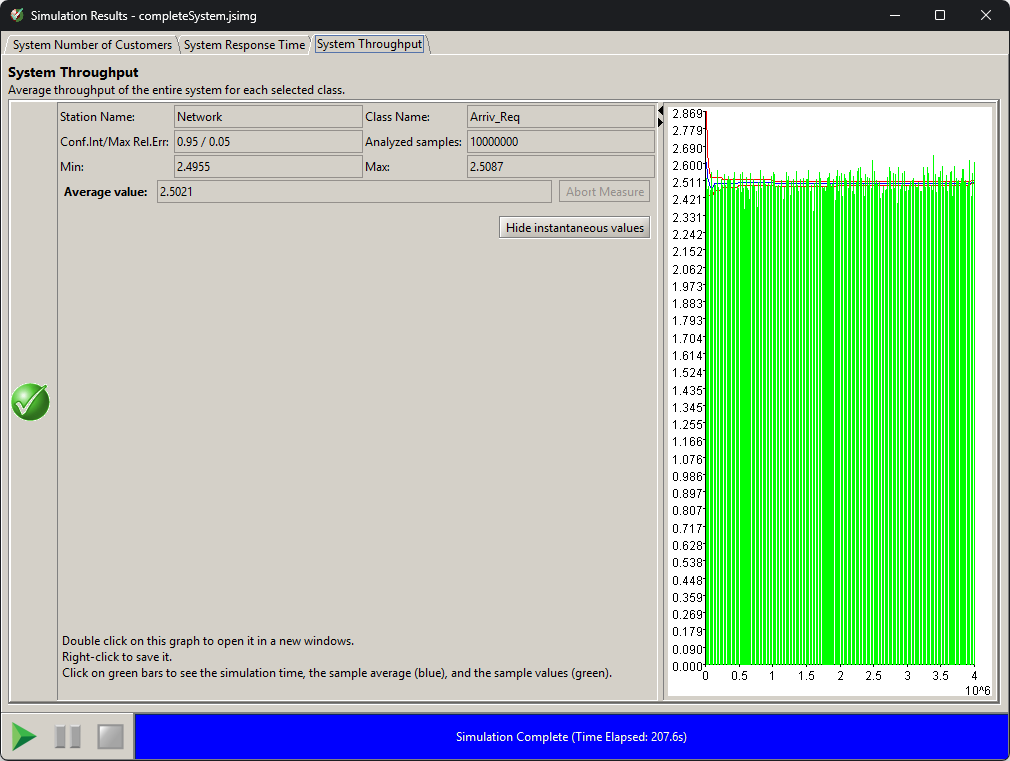
\includegraphics[
        width=0.88\textwidth,
        trim=0 380 0 25,
        clip
    ]{../data/simulation/simple_system/throughput}

    \caption{Risultati JSIM per la validazione dell'architettura Web Server e Spike Server.}
    \label{fig:jsim_system_validation}
\end{figure}

La campagna Java definitiva è stata configurata con $4096$ batch da $4096$ job. I risultati in Tabella~\ref{tab:validation_system_comparison} mostrano una buona aderenza tra le due implementazioni indipendenti. Il throughput, indice particolarmente sensibile alla corretta conservazione del flusso, differisce solo dello $0.34\%$ e gli intervalli di confidenza si sovrappongono. Anche il numero medio di job nel sistema mantiene uno scarto contenuto, pari a circa $1.31\%$, con sovrapposizione tra gli intervalli. Il tempo di risposta medio del simulatore Java risulta leggermente più alto di quello JSIM ($0.9157\text{ s}$ contro $0.9043\text{ s}$), con uno scostamento relativo pari a circa $1.26\%$: tale differenza è coerente con la semplificazione adottata nel modello JSIM per approssimare il router a soglia e con la diversa logica di arresto statistico usata dai due strumenti.

\begin{table}[htbp]
    \centering
    \small
    \renewcommand{\arraystretch}{1.3}
    \begin{tabular}{lcccc}
        \hline
        \textbf{Metrica} & \textbf{Simulatore Java} & \textbf{CI Java 95\%} & \textbf{JSIM} & \textbf{CI JSIM 95\%} \\ \hline
        $E[T_s]$         & $0.9157\text{ s}$        & $[0.9121, 0.9194]$    & $0.9043\text{ s}$ & $[0.8996, 0.9089]$ \\
        $E[N_s]$         & $2.3048$                 & $[2.2933, 2.3162]$    & $2.2749$          & $[2.2531, 2.2968]$ \\
        $X$              & $2.5106\text{ job/s}$    & $[2.5057, 2.5156]$    & $2.5021\text{ job/s}$ & $[2.4955, 2.5087]$ \\ \hline
    \end{tabular}
    \caption{Confronto di validazione tra simulatore Java e JSIM sull'architettura Web Server e Spike Server.}
    \label{tab:validation_system_comparison}
\end{table}

Il report Java conferma inoltre che lo scenario è rimasto effettivamente statico rispetto agli autoscaler: tutte le azioni di \textit{Scale Out}, \textit{Scale In}, \textit{Scale Up} e \textit{Scale Down} hanno media nulla, mentre il numero medio di server attivi è pari a $1.0000$. L'utilizzazione media dello Spike Server risulta pari a $0.0225$, segnale che la risorsa ausiliaria viene attivata solo durante gli episodi di congestione locale. Questa evidenza è coerente con la finalità della validazione: il livello di picco non deve alterare il carico ordinario, ma deve intervenire come percorso di sfogo quando la soglia del Web Server viene raggiunta. Il leggero scostamento sul tempo di risposta non è quindi un risultato imprevisto, ma l'effetto atteso della modellazione approssimata della soglia in JSIM rispetto alla decisione evento-per-evento implementata nel simulatore Java.

Nel complesso, la validazione esterna mostra che il simulatore implementato replica correttamente sia il comportamento di una stazione singola ad alta variabilità, sia l'effetto prestazionale aggregato dell'architettura a due livelli. Le differenze residue sono contenute e spiegabili dalle diverse astrazioni richieste per rappresentare in JSIM la strategia di routing a soglia; pertanto il modello sviluppato può essere considerato adeguato per le successive campagne di analisi e dimensionamento.

\clearpage


% =========================================================================
% RISULTATI
% =========================================================================
\section{Risultati e Analisi}
In questo capitolo vengono presentati e discussi i risultati ottenuti dalle diverse campagne di simulazione, evidenziando il raggiungimento degli obiettivi prefissati e analizzando le prestazioni del sistema sotto diversi scenari operativi. L'esposizione segue lo stesso percorso sperimentale adottato nel progetto: prima vengono fissati i parametri di dimensionamento, poi viene valutata l'architettura completa in termini di costo, dinamica transitoria e robustezza rispetto alla variabilità del carico, infine viene discusso il miglioramento ottenuto introducendo una banda di isteresi nel meccanismo di dirottamento.


\subsection{Dimensionamento}

\paragraph{Ottimizzazione delle Politiche di Instradamento}
L'ottimizzazione delle politiche di instradamento è stata condotta tramite la classe \texttt{RoutingPolicyObjective}, isolando il solo effetto del bilanciamento del carico sul cluster ordinario. Lo scenario sperimentale è stato configurato con 4 Web Server statici, Spike Server abilitato, assenza completa di meccanismi di scaling orizzontale e verticale, carico iperesponenziale $H_2/H_2$ con $\lambda = 5.0\text{ job/s}$, $\mu = 4.0\text{ job/s}$ per singolo server e coefficiente di variazione pari a $C_V = 4.0$ sia per gli interarrivi sia per i tempi di servizio. La stima preliminare dei Batch Means è stata effettuata su un'architettura rappresentativa dello stesso esperimento; il metodo ACF ha individuato un cutoff pari a $284$, con batch da $2840$ job, $1760$ batch e lag-1 ACF pari a $0.0453$, mentre il metodo dinamico ha raggiunto lag-1 ACF pari a $-0.0394$ con batch da $131072$ job e $32$ batch. Il candidato selezionato è stato quello derivato dal metodo ACF, poiché caratterizzato dal maggior numero di osservazioni utili e dalla minima \textit{Half-Width} sul tempo di risposta. Come da criterio metodologico adottato, i parametri sono stati quindi arrotondati alla successiva potenza di 2, ottenendo la configurazione finale di $k = 4096$ batch da $b = 2048$ job ciascuno.

Il confronto ha coinvolto le quattro strategie \textit{Round Robin}, \textit{Random}, \textit{Least Loaded} e \textit{Power of Two Choices}. I risultati quantitativi, riportati in Tabella~\ref{tab:routing_policy_results}, mostrano una gerarchia netta e stabile. La politica \textbf{Least Loaded} risulta la migliore in assoluto, con un tempo medio di risposta pari a $0.2843\text{ s}$, una \textit{Half-Width} di appena $0.0011\text{ s}$ e una deviazione standard pari a $0.0243\text{ s}$; rispetto a \textit{Round Robin} riduce la latenza media di circa il $24.7\%$, mentre il guadagno sale a circa il $33.3\%$ rispetto alla politica \textit{Random}. La tecnica \textit{Power of Two Choices} si colloca in seconda posizione con $R_0 = 0.3147\text{ s}$, confermando di essere un compromesso molto efficace tra qualità del bilanciamento e costo informativo, mentre \textit{Random} risulta la politica meno efficiente a causa dell'assenza di qualunque meccanismo di correzione delle collisioni locali.

Il risultato osservato è coerente con l'aspettativa teorica. In uno scenario con server omogenei e carico altamente variabile, la politica che osserva direttamente il numero di job residenti deve ridurre più efficacemente la congestione locale; al contrario, una politica cieca come \textit{Random} può produrre collisioni temporanee anche quando esiste capacità libera altrove. Non emergono quindi anomalie sperimentali: la classifica ottenuta riflette il diverso livello informativo disponibile al router.
\begin{table}[H]
    \centering
    \small
    \renewcommand{\arraystretch}{1.3}
    \begin{tabular}{lcccc}
        \hline
        \textbf{Politica di Routing} & \textbf{$R_0$ Medio [s]} & \textbf{HW [s]} & \textbf{CI 95\% $R_0$ [s]} & \textbf{StdDev [s]} \\ \hline
        Round Robin                  & $0.3776$                & $0.0019$        & $[0.3757, 0.3795]$         & $0.0441$            \\
        Least Loaded                 & $0.2843$                & $0.0011$        & $[0.2832, 0.2854]$         & $0.0243$            \\
        Random                       & $0.4262$                & $0.0020$        & $[0.4242, 0.4282]$         & $0.0465$            \\
        Power of Two Choices         & $0.3146$                & $0.0012$        & $[0.3134, 0.3158]$         & $0.0280$            \\ \hline
    \end{tabular}
    \caption{Confronto prestazionale tra le politiche di instradamento sul cluster statico a 4 Web Server.}
    \label{tab:routing_policy_results}
\end{table}

L'evidenza grafica in Figura~\ref{fig:routing_policy_comparison} conferma che il vantaggio di \textit{Least Loaded} non si limita a un semplice abbassamento della media, ma si traduce anche in una sensibile contrazione della dispersione statistica. Questo punto è particolarmente rilevante alla luce della disciplina di scheduling adottata nei server, di tipo \textit{Processor Sharing}: tale meccanismo tende infatti a ripartire equamente la capacità di servizio tra i job concorrenti, attenuando l'iniquità individuale rispetto a una coda FCFS, ma non elimina affatto il costo della congestione locale. Quando una politica di routing concentra troppi job sullo stesso nodo, ogni nuovo arrivo entra immediatamente in competizione con un numero maggiore di richieste già residenti e il rallentamento si propaga a tutti i task presenti su quel server. Per questa ragione, anche in presenza di \textit{Processor Sharing}, la qualità dell'informazione usata dal router resta determinante: \textit{Least Loaded} minimizza la concorrenza locale osservando lo stato istantaneo del sistema, \textit{Power of Two Choices} ne cattura una versione approssimata ma già molto efficace, mentre \textit{Round Robin} e soprattutto \textit{Random} subiscono più facilmente sbilanciamenti transitori che si riflettono in una maggiore varianza del tempo di risposta.

\begin{figure}[H]
    \centering
    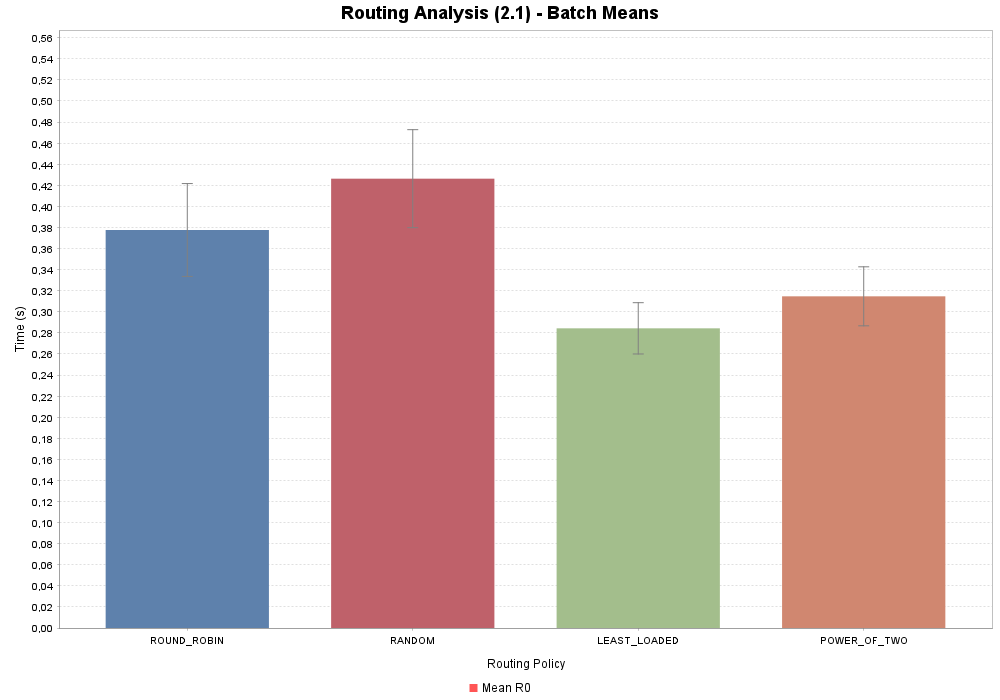
\includegraphics[width=0.74\textwidth]{../data/objective/routing_policy_comparison}
    \caption{Confronto grafico delle prestazioni delle politiche di routing in termini di tempo medio di risposta e dispersione statistica.}
    \label{fig:routing_policy_comparison}
\end{figure}

Nel complesso, questa campagna sperimentale giustifica la scelta di \textit{Least Loaded} come politica di riferimento per le successive analisi di dimensionamento: essa è la strategia che sfrutta meglio la parallelizzazione del cluster, riduce la probabilità di micro-congestioni sui singoli nodi e stabilizza maggiormente il comportamento del sistema sotto carico fortemente variabile. \textit{Power of Two Choices} rimane tuttavia una valida alternativa qualora si voglia ridurre l'overhead di monitoraggio, accettando un degrado prestazionale contenuto.

\paragraph{Ottimizzazione della Soglia di Dirottamento $SI_{max}$}
La scelta della soglia di dirottamento verso lo Spike Server è stata condotta tramite la classe \texttt{SiMaxEstimationObjective}, con l'obiettivo di individuare il massimo valore di $SI_{max}$ compatibile con il vincolo prestazionale imposto dallo SLA. Lo scenario di prova è stato mantenuto volutamente stazionario, con un singolo Web Server ordinario, Spike Server attivo, scaling disabilitato e carico iperesponenziale $H_2/H_2$ ad alta variabilità. La campagna \textit{what-if} ha esplorato valori di $SI_{max}$ compresi tra 10 e 150, osservando congiuntamente il tempo medio di risposta $R_0$, la quota di job dirottati e l'utilizzazione media dello Spike Server.

Anche per questa campagna è stata condotta una stima preliminare dei Batch Means. Il metodo ACF ha rilevato un cutoff pari a $60$, con batch da $600$ job, $8333$ batch e lag-1 ACF pari a $0.0683$; il metodo dinamico ha invece prodotto batch da $2048$ job, $48$ batch e lag-1 ACF pari a $0.0020$. La configurazione finale è stata scelta in modo conservativo, privilegiando la stabilità degli intervalli di confidenza nella regione prossima alla soglia SLA.

I risultati numerici, sintetizzati nella Tabella~\ref{tab:simax_estimation_results}, mostrano un comportamento molto netto. All'aumentare di $SI_{max}$, il router tollera livelli di congestione locale sempre più elevati prima di attivare il percorso ausiliario; di conseguenza la percentuale di job deviati e l'utilizzazione dello Spike Server decrescono rapidamente nella prima parte della curva, mentre il tempo medio di risposta cresce in modo monotono. Questo trade-off è atteso: soglie più basse proteggono in maniera aggressiva il server ordinario, ma trasferiscono una porzione maggiore del carico alla risorsa di picco; soglie più alte, al contrario, riducono il ricorso allo Spike Server ma espongono il nodo principale a fenomeni di saturazione prolungata, che in presenza di scheduling \textit{Processor Sharing} penalizzano simultaneamente tutti i job residenti.

\begin{table}[H]
    \centering
    \small
    \renewcommand{\arraystretch}{1.3}
    \begin{tabular}{lccccc}
        \hline
        \textbf{$SI_{max}$} & \textbf{$R_0$ Medio [s]} & \textbf{HW [s]} & \textbf{CI 95\% $R_0$ [s]} & \textbf{Job Deviati [\%]} & \textbf{Util. Spike [\%]} \\ \hline
        $10$   & $1.4130$  & $0.0050$ & $[1.4080, 1.4181]$   & $30.06$ & $38.73$ \\
        $20$   & $2.5786$  & $0.0079$ & $[2.5707, 2.5865]$   & $23.65$ & $30.80$ \\
        $30$   & $3.9709$  & $0.0124$ & $[3.9585, 3.9833]$   & $21.34$ & $27.90$ \\
        $40$   & $5.5279$  & $0.0172$ & $[5.5107, 5.5451]$   & $20.38$ & $26.74$ \\
        $50$   & $7.2009$  & $0.0216$ & $[7.1793, 7.2225]$   & $19.98$ & $26.29$ \\
        $60$   & $8.9588$  & $0.0259$ & $[8.9329, 8.9847]$   & $19.85$ & $26.13$ \\
        $70$   & $10.7680$ & $0.0303$ & $[10.7377, 10.7982]$ & $19.83$ & $26.06$ \\
        $80$   & $12.6091$ & $0.0346$ & $[12.5745, 12.6437]$ & $19.83$ & $26.05$ \\
        $100$  & $16.3577$ & $0.0435$ & $[16.3142, 16.4011]$ & $19.85$ & $26.05$ \\
        $150$  & $25.9110$ & $0.0676$ & $[25.8434, 25.9786]$ & $19.86$ & $26.10$ \\ \hline
    \end{tabular}
    \caption{Analisi di sensitività della soglia $SI_{max}$ in regime stazionario.}
    \label{tab:simax_estimation_results}
\end{table}

La Figura~\ref{fig:simax_estimation} rende ancora più evidente la struttura del compromesso. Il comportamento atteso era una crescita monotona del tempo di risposta al crescere della soglia, accompagnata da una riduzione progressiva del ricorso allo Spike Server; i risultati confermano questa lettura. Il tempo medio di risposta cresce in modo pressoché lineare fino ad avvicinarsi alla frontiera dello SLA, mentre la curva di utilizzazione dello Spike Server subisce una rapida discesa iniziale e poi si assesta su un plateau quasi stazionario attorno al $25\%$. Questo asintoto è importante dal punto di vista progettuale: oltre un certo valore della soglia, il sistema non ottiene più un risparmio significativo nell'uso della risorsa di picco, ma continua invece a pagare un costo crescente in termini di latenza.

\begin{figure}[H]
    \centering
    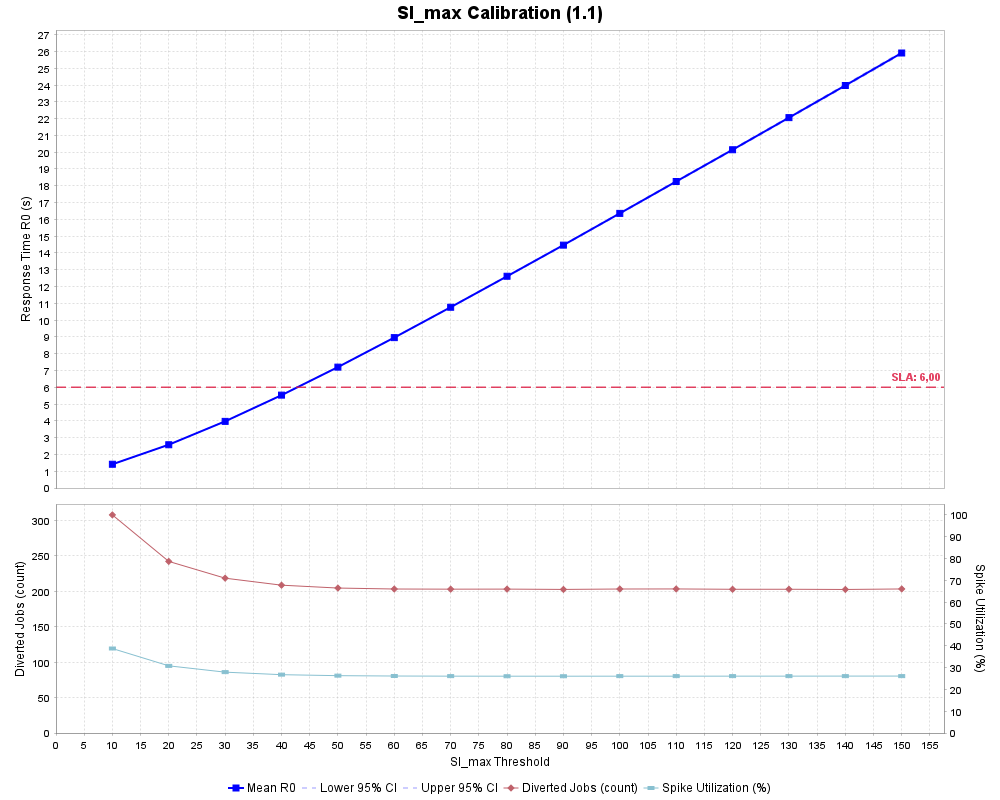
\includegraphics[width=0.86\textwidth]{../data/objective/simax_estimation}
    \caption{Trade-off tra tempo di risposta, quota di job dirottati e utilizzazione dello Spike Server al variare di $SI_{max}$.}
    \label{fig:simax_estimation}
\end{figure}

Alla luce di queste evidenze, la scelta finale ricade su \textbf{$SI_{max} = 40$}. Tale valore rappresenta infatti il punto limite immediatamente precedente al superamento della soglia di $6\text{ s}$ fissata dal nostro SLA: con $SI_{max} = 40$ il sistema mantiene ancora $R_0 = 5.5279\text{ s}$ e un intervallo di confidenza $[5.5107, 5.5451]\text{ s}$ interamente al di sotto del vincolo, mentre già al passo successivo, $SI_{max} = 50$, il tempo medio di risposta sale a $7.2009\text{ s}$ violando il requisito di servizio. Inoltre, $SI_{max} = 40$ si colloca nella regione in cui la curva di utilizzazione dello Spike Server si è ormai stabilizzata attorno al $26\%$, rendendo non conveniente spostare ulteriormente in alto la soglia. Questa configurazione costituisce quindi il miglior punto di equilibrio tra protezione del Web Server principale, contenimento dell'uso dello Spike Server e rispetto rigoroso del vincolo SLA a regime.

\paragraph{Scaling Verticale e Sizing dell'Incremento}
Il dimensionamento dello \textit{speedup} verticale dello Spike Server è stato analizzato tramite la classe \texttt{VerticalStepSizingObjective}. L'obiettivo dell'esperimento era verificare se un incremento più aggressivo della velocità di servizio della risorsa ausiliaria producesse un beneficio misurabile sul tempo medio di risposta, una volta fissata la soglia di dirottamento a $SI_{max} = 40$. Lo scenario è stato mantenuto coerente con la precedente fase di dimensionamento: singolo Web Server ordinario, Spike Server abilitato, scaling orizzontale disabilitato, scaling verticale attivo e carico iperesponenziale ad alta variabilità. La campagna è stata eseguita con $16384$ batch da $1024$ job, scartando una fase iniziale di warm-up pari a $2048$ job.

La calibrazione statistica preliminare ha rilevato, con il metodo ACF, un cutoff pari a $486$, batch da $4860$ job, $1028$ batch e lag-1 ACF pari a $0.0252$. Il metodo dinamico ha invece raggiunto lag-1 ACF pari a $0.0059$, ma con intervalli di confidenza più ampi sulla media. Anche in questo caso la scelta finale dei parametri privilegia quindi una stima più regolare del regime stazionario.

I risultati riportati in Tabella~\ref{tab:vertical_step_sizing_results} mostrano che la variazione dell'incremento di velocità non introduce alcun miglioramento prestazionale sostanziale. L'aspettativa iniziale era osservare almeno una riduzione moderata di $R_0$ per speedup più elevati, nel caso in cui lo Spike Server fosse il collo di bottiglia dominante; l'esito sperimentale mostra invece che tale ipotesi non è verificata. Il tempo medio di risposta resta infatti compreso in un intervallo estremamente ristretto, tra $5.5103\text{ s}$ e $5.5162\text{ s}$, e tutti gli intervalli di confidenza al $95\%$ risultano completamente sovrapposti. Anche il grafico in Figura~\ref{fig:vertical_step_sizing} conferma l'andamento sostanzialmente piatto della curva di $R_0$: l'aumento della capacità verticale disponibile non modifica in modo apprezzabile il comportamento globale del sistema, perché il collo di bottiglia dominante non è la velocità istantanea dello Spike Server, ma il momento in cui il traffico viene effettivamente dirottato dal Web Server ordinario.

\begin{table}[H]
    \centering
    \small
    \renewcommand{\arraystretch}{1.3}
    \begin{tabular}{lccc}
        \hline
        \textbf{Incremento Velocità} & \textbf{$R_0$ Medio [s]} & \textbf{Half-Width [s]} & \textbf{CI 95\% $R_0$ [s]} \\ \hline
        $0.50$ & $5.5162$ & $0.0193$ & $[5.4969, 5.5355]$ \\
        $1.00$ & $5.5132$ & $0.0193$ & $[5.4939, 5.5325]$ \\
        $1.50$ & $5.5120$ & $0.0192$ & $[5.4928, 5.5312]$ \\
        $2.00$ & $5.5113$ & $0.0192$ & $[5.4921, 5.5305]$ \\
        $3.00$ & $5.5107$ & $0.0192$ & $[5.4915, 5.5299]$ \\
        $4.00$ & $5.5104$ & $0.0192$ & $[5.4912, 5.5296]$ \\
        $5.00$ & $5.5103$ & $0.0192$ & $[5.4911, 5.5295]$ \\ \hline
    \end{tabular}
    \caption{Analisi dell'impatto dell'incremento di velocità verticale sul tempo medio di risposta.}
    \label{tab:vertical_step_sizing_results}
\end{table}

\begin{figure}[H]
    \centering
    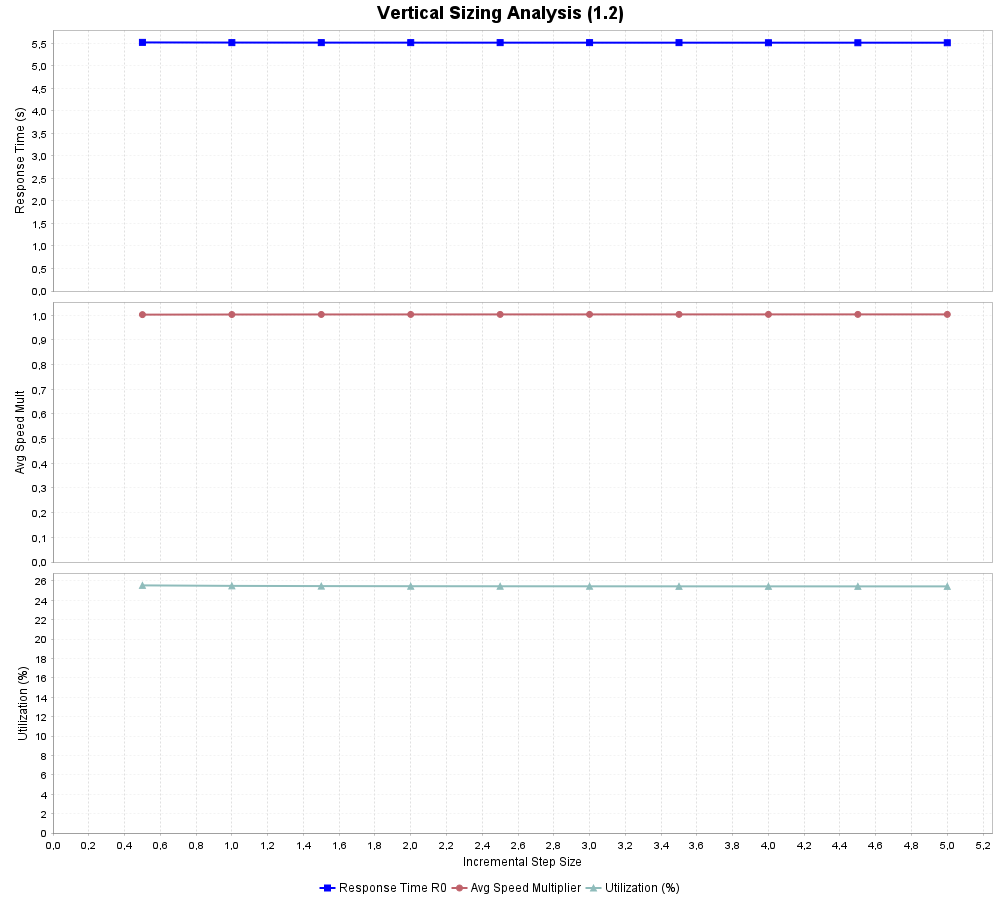
\includegraphics[width=0.86\textwidth]{../data/objective/vertical_step_sizing}
    \caption{Effetto dell'incremento di velocità verticale su tempo di risposta, velocità media e utilizzazione dello Spike Server.}
    \label{fig:vertical_step_sizing}
\end{figure}

Questa evidenza porta a una conclusione progettuale precisa: aumentare ulteriormente lo speedup verticale non è conveniente. Dal punto di vista economico, una capacità di picco più elevata comporterebbe un costo potenziale maggiore senza produrre una riduzione statisticamente significativa della latenza media. Per questo motivo si è scelto di adottare un incremento di velocità pari a \textbf{1.0}, corrispondente a un raddoppio della potenza disponibile quando lo scaling verticale viene attivato. Tale configurazione rappresenta la scelta più sobria e difendibile: garantisce una risposta sufficiente nelle fasi di picco, evita sovradimensionamenti inutili e mantiene il costo operativo dello Spike Server sotto controllo.

\paragraph{Scaling Orizzontale e Identificazione delle Soglie}
La stima dei parametri per lo scaling orizzontale è stata condotta tramite la classe \texttt{HorizontalScalingEstimationObjective}. Il parametro superiore di intervento, cioè la soglia di \textit{Scale Out}, è stato fissato direttamente al valore del vincolo SLA, pari a $R^{max}=6.0\text{ s}$. Questa scelta è coerente con una politica di controllo parsimoniosa: l'aumento del numero di Web Server viene attivato solo quando il tempo medio di risposta supera effettivamente il limite prestazionale concordato, evitando espansioni inutili quando il sistema si trova ancora all'interno dello SLA. Qualora si desiderasse un comportamento più reattivo e prudenziale, lo stesso parametro potrebbe essere abbassato leggermente, anticipando lo \textit{Scale Out} prima del raggiungimento formale della soglia critica e aumentando così il margine di sicurezza rispetto a variazioni improvvise del carico.

L'obiettivo dell'esperimento non è stato quello di osservare direttamente la dinamica del controller, bensì di ricostruire la frontiera prestazionale delle configurazioni statiche da 1 a 5 Web Server al variare del tasso di arrivo $\lambda$. Per ogni coppia $(\lambda, N)$ è stata preliminarmente eseguita una verifica di convergenza a orizzonte finito tramite repliche indipendenti; solo le configurazioni classificate come convergenti sono state poi analizzate a regime con Batch Means, usando il numero di job di convergenza come \textit{warm-up}. Le configurazioni non convergenti o inconclusive sono state escluse dalla stima steady-state e riportate esplicitamente nel CSV e nel grafico.

I risultati, sintetizzati nella Tabella~\ref{tab:horizontal_scaling_results}, evidenziano che con SLA pari a $6\text{ s}$ la regione ammissibile rimane coerente con il carico nominale del progetto, ma diventa più selettiva nei regimi ad alta intensità. Il comportamento atteso è quello tipico di una frontiera di capacità: a parità di $\lambda$, l'aumento del numero di Web Server deve ridurre il tempo di risposta, mentre a parità di server l'incremento del carico deve avvicinare progressivamente il sistema alla saturazione. I risultati seguono questa struttura. Per carichi prossimi a $\lambda = 5$, che rappresentano il centro dello scenario di riferimento, un singolo Web Server è ancora sostenibile, con $R_0 = 5.5212\text{ s}$ e intervallo di confidenza $[5.4926, 5.5498]\text{ s}$ interamente sotto soglia. Anche a $\lambda = 6.5$ la configurazione a un solo server resta formalmente ammissibile, con $R_0 = 5.8807\text{ s}$, ma il margine rispetto allo SLA diventa molto ridotto. L'aggiunta di un secondo server riduce drasticamente la latenza, portandola a $0.7296\text{ s}$ per $\lambda = 5$ e a $1.5517\text{ s}$ per $\lambda = 6.5$, mostrando che in questa regione due nodi sono prestazionalmente conservativi.

\begin{table}[H]
    \centering
    \small
    \renewcommand{\arraystretch}{1.3}
    \begin{tabular}{lcccc}
        \hline
        \textbf{$\lambda$} & \textbf{1 WS} & \textbf{2 WS} & \textbf{3 WS} & \textbf{5 WS} \\ \hline
        $5.00$  & $5.5130 \pm 0.0283$ & $0.7316 \pm 0.0077$ & $0.3563 \pm 0.0012$ & $0.2614 \pm 0.0008$ \\
        $6.50$  & $5.8808 \pm 0.0334$ & $1.5519 \pm 0.0309$ & $0.4608 \pm 0.0022$ & $0.2757 \pm 0.0010$ \\
        $8.00$  & \textit{INC.}        & $4.4585 \pm 0.0878$ & $0.6542 \pm 0.0046$ & $0.2978 \pm 0.0012$ \\
        $9.50$  & \textit{Skip}        & $6.5519 \pm 0.0418$ & $1.0545 \pm 0.0117$ & $0.3303 \pm 0.0015$ \\
        $11.00$ & \textit{Skip}        & $7.7255 \pm 0.1140$ & \textit{INC.}        & $0.3776 \pm 0.0020$ \\ \hline
    \end{tabular}
    \caption{Sintesi dei risultati di dimensionamento orizzontale con SLA pari a $6\text{ s}$. I valori riportano $R_0 \pm$ Half-Width; \textit{INC.} indica configurazione inconclusiva nella verifica di convergenza, mentre \textit{Skip} indica configurazioni saltate per monotonicità del carico.}
    \label{tab:horizontal_scaling_results}
\end{table}

La soglia di \textit{Scale In} deve quindi essere scelta in modo da favorire il ritorno a una sola unità quando il carico nominale è prossimo a $\lambda = 5$, ma senza autorizzare contrazioni pericolose nella regione in cui un singolo Web Server non è più sostenibile. Poiché $R^{max}=6.0\text{ s}$ rappresenta già la soglia superiore di violazione dello SLA, non sarebbe corretto usare lo stesso valore anche come soglia di riduzione: verrebbe infatti annullata la banda di isteresi tra espansione e contrazione, rendendo il controller troppo incline a rimuovere risorse appena il sistema rientra formalmente sotto il limite. Alla luce dei risultati aggiornati, una scelta più coerente per lo scenario principale è \textbf{$R^{min}=3.5\text{ s}$}. Questo valore mantiene un margine sufficiente rispetto allo SLA, evita oscillazioni eccessive vicino alla soglia critica e consente comunque il ritorno verso configurazioni più economiche quando il carico si trova nella regione ordinaria del progetto.

\begin{figure}[H]
    \centering
    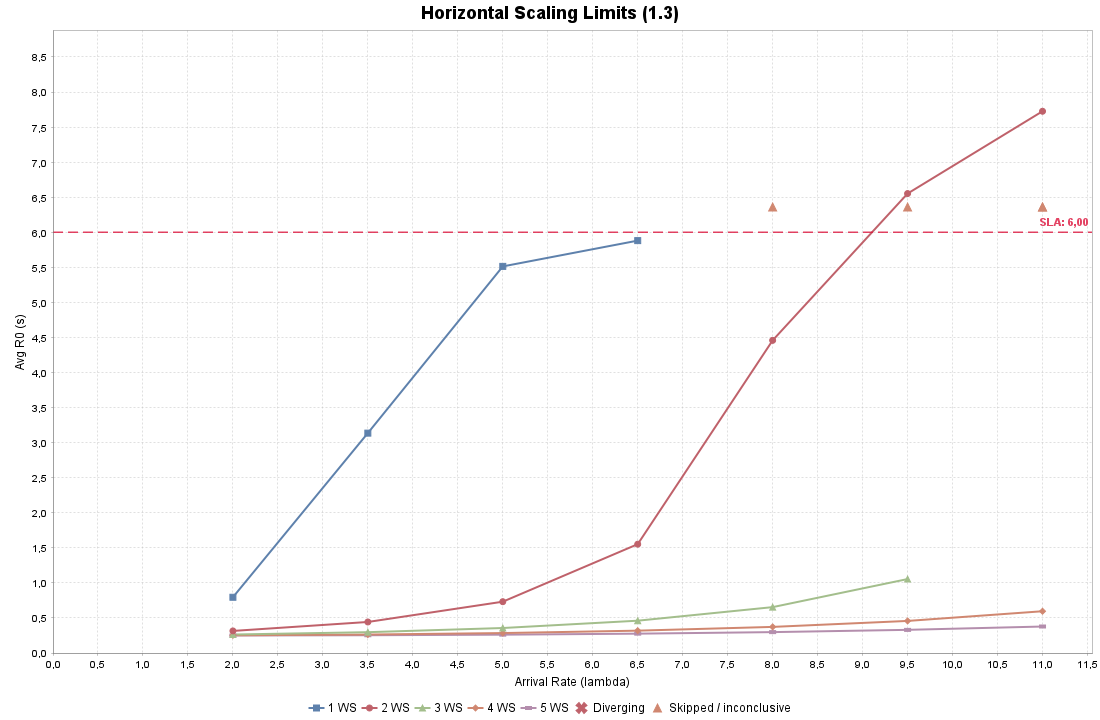
\includegraphics[width=0.86\textwidth]{../data/objective/horizontal_parameter_estimation}
    \caption{Frontiera prestazionale delle configurazioni statiche da 1 a 5 Web Server al variare di $\lambda$, con SLA pari a $6\text{ s}$. I marker sopra la soglia indicano configurazioni non simulate a regime poiché non convergenti o saltate per monotonicità.}
    \label{fig:horizontal_parameter_estimation}
\end{figure}

Per scenari di carico più elevato, prossimi a $\lambda = 9.5$ o $\lambda = 11$, la soglia a $6\text{ s}$ modifica sensibilmente l'interpretazione. Due server non garantiscono più il rispetto del vincolo, poiché producono rispettivamente $R_0 = 6.5519\text{ s}$ e $R_0 = 7.7255\text{ s}$; al contrario, cinque server mantengono la latenza entro margini molto ampi, con $R_0 = 0.3303\text{ s}$ a $\lambda = 9.5$ e $R_0 = 0.3776\text{ s}$ a $\lambda = 11$. La configurazione a tre server resta valida fino a $\lambda=9.5$, ma nello scenario più intenso risulta inconclusiva nella verifica di convergenza; per questo motivo, in presenza di workload persistentemente elevati, una soglia di \textit{Scale In} tra $1.5\text{ s}$ e $2.0\text{ s}$ rimarrebbe la scelta più conservativa, perché manterrebbe più facilmente tre o più server attivi e offrirebbe maggiore margine rispetto a burst improvvisi. Il valore $R^{min}=3.5\text{ s}$ va invece interpretato come una scelta coerente con un profilo di carico centrato su $\lambda \simeq 5$, non come soglia ottimale per workload persistentemente elevati.

In conclusione, il dimensionamento dello scaling orizzontale dipende dal carico nominale atteso. Nel caso di studio principale, centrato su valori di $\lambda$ prossimi a 5 e con SLA pari a $6\text{ s}$, la scelta \textbf{$R^{min}=3.5\text{ s}$} è coerente con una politica orientata al contenimento dei costi: preserva il risparmio economico nei regimi sostenibili da un solo Web Server, ma conserva una banda di isteresi rispetto a $R^{max}$ sufficiente a evitare rimozioni premature. Per workload persistentemente più aggressivi, invece, la soglia deve essere abbassata ulteriormente, indicativamente nell'intervallo $1.5$--$2.0\text{ s}$, accettando un costo infrastrutturale maggiore in cambio di una maggiore robustezza operativa. Le verifiche di convergenza hanno mostrato warm-up molto variabili: le configurazioni stabili convergono tipicamente tra $60000$ e $240000$ job, mentre i casi prossimi alla saturazione possono arrivare a $940000$ job senza classificazione conclusiva. Questo risultato conferma la necessità di usare il job di convergenza stimato come warm-up della successiva analisi Batch Means.
\subsection{Analisi}

\paragraph{Analisi Economica e Trade-off dei Costi}
L'analisi dei costi operativi è stata implementata nella classe \texttt{CostOptimizationObjective}, mantenendo fisso il limite superiore $R^{max}=6.0\text{ s}$ e valutando congiuntamente diverse soglie di \textit{Scale In} e diversi tempi di \textit{Cooldown}. La campagna è stata costruita sulla configurazione completa del sistema: politica \textit{Least Loaded}, $SI_{max}=40$, soglia inferiore di dirottamento coerente con la banda scelta, scaling orizzontale e verticale abilitati, \textit{Window Size} pari a $100\text{ s}$ e \textit{Cooldown} variabile tra $5$, $10$, $50$ e $100\text{ s}$.

Per questa campagna sperimentale la calibrazione dei Batch Means è stata effettuata tramite l'approccio dinamico, poiché il metodo ACF richiedeva run molto lunghe e costose. La stima preliminare ha individuato un cutoff ACF pari a $1221$, con $409$ batch da $12210$ job e lag-1 ACF pari a $-0.0531$; il metodo dinamico ha invece raggiunto lag-1 ACF pari a $0.0050$ con $34$ batch da $4096$ job e precisione relativa pari a $0.0293$. L'esperimento finale usa quindi un arrotondamento superiore, pari a $64$ batch da $8192$ job, e un warm-up prudenziale pari a $350000$ job. La stima di convergenza a orizzonte finito aveva indicato stabilizzazione già a $60000$ job, con $R_0=3.3309\text{ s}$ e HW pari a $0.0343\text{ s}$; la scelta di amplificare il warm-up riduce ulteriormente il rischio di includere transitori residui.

Il modello economico adottato considera un costo fisso per ogni Web Server attivo e un costo variabile per lo Spike Server proporzionale sia alla sua utilizzazione sia alla velocità media allocata:
\[
    C_{tot} = \bar{N}\,C_{WS} + \bar{U}_{spike}\,\bar{S}_{spike}\,C_{CPU}.
\]
In questo modo il costo della capacità orizzontale viene pagato ogni volta che un Web Server resta mediamente acceso, mentre il costo della risorsa di picco cresce solo quando lo Spike Server viene effettivamente utilizzato e accelerato.

I risultati, sintetizzati nella Tabella~\ref{tab:cost_tradeoff_results} e nelle Figure~\ref{fig:cost_analysis_cd5}--\ref{fig:cost_analysis_cd100}, confermano il trade-off atteso. Soglie di \textit{Scale In} basse, come $R^{min}=1.0\text{ s}$ o $R^{min}=2.0\text{ s}$, mantengono più a lungo server aggiuntivi nel cluster: questo abbassa il tempo medio di risposta, soprattutto ad alto carico, ma aumenta sensibilmente il costo medio a causa del maggior numero di Web Server attivi. Al contrario, soglie più permissive, come $R^{min}=5.0\text{ s}$ o $R^{min}=6.0\text{ s}$, riducono il costo operativo perché favoriscono una contrazione più rapida del cluster; il prezzo pagato è un tempo di risposta più elevato, pur rimanendo entro il vincolo SLA in tutti gli scenari simulati.

L'esito è quindi in linea con il comportamento atteso del controller: abbassare la soglia di \textit{Scale In} rende il sistema più prudente e prestazionalmente robusto, ma più costoso; alzarla spinge invece verso configurazioni più economiche, accettando una latenza media maggiore. La campagna serve proprio a quantificare questo compromesso, non a individuare un minimo assoluto valido per qualunque profilo di traffico.

\begin{table}[H]
    \centering
    \small
    \renewcommand{\arraystretch}{1.25}
    \begin{tabular}{lcccc}
        \hline
        \textbf{$R^{min}$} & \textbf{Cooldown [s]} & \textbf{$\overline{C}_{tot}$} & \textbf{$\overline{R}_0$ [s]} & \textbf{$R_0(\lambda=11)$ [s]} \\ \hline
        $1.0$ & $10$ & $5.541$ & $2.860$ & $3.262$ \\
        $2.0$ & $10$ & $5.040$ & $3.106$ & $3.642$ \\
        $5.0$ & $10$ & $4.302$ & $3.470$ & $4.126$ \\
        $6.0$ & $10$ & $4.213$ & $3.542$ & $4.207$ \\ \hline
    \end{tabular}
    \caption{Sintesi del compromesso costo-prestazioni con \textit{Cooldown} fissato a $10\text{ s}$. Le medie sono calcolate sui valori di $\lambda$ simulati.}
    \label{tab:cost_tradeoff_results}
\end{table}

\begin{figure}[H]
    \centering
    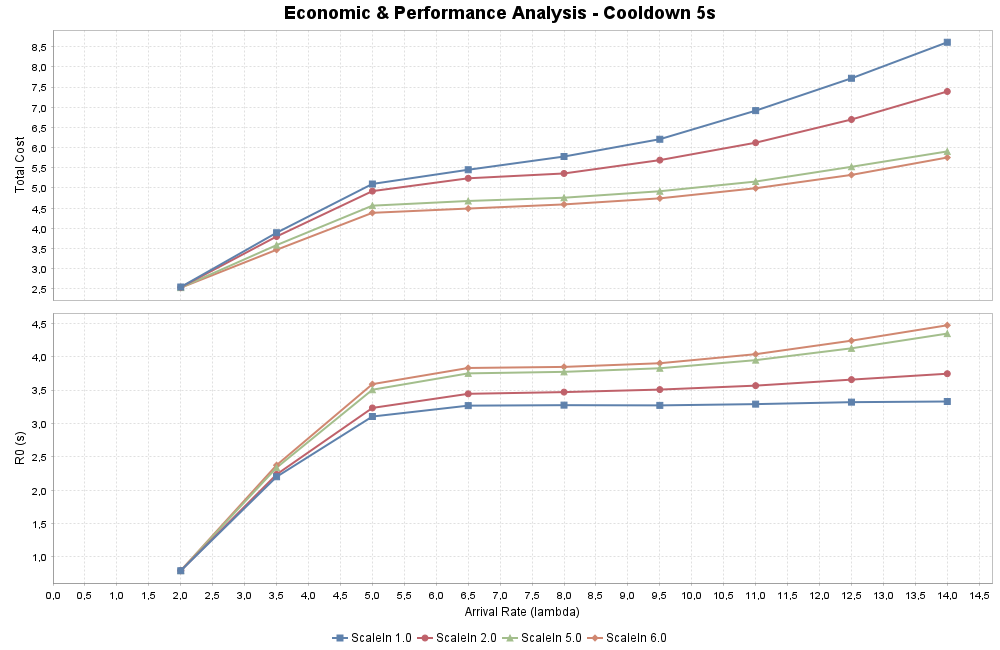
\includegraphics[width=0.72\textwidth]{../data/objective/cost/cost_analysis_cooldown_5s}
    \caption{Andamento del costo totale e del tempo medio di risposta con \textit{Cooldown} pari a $5\text{ s}$.}
    \label{fig:cost_analysis_cd5}
\end{figure}

\begin{figure}[H]
    \centering
    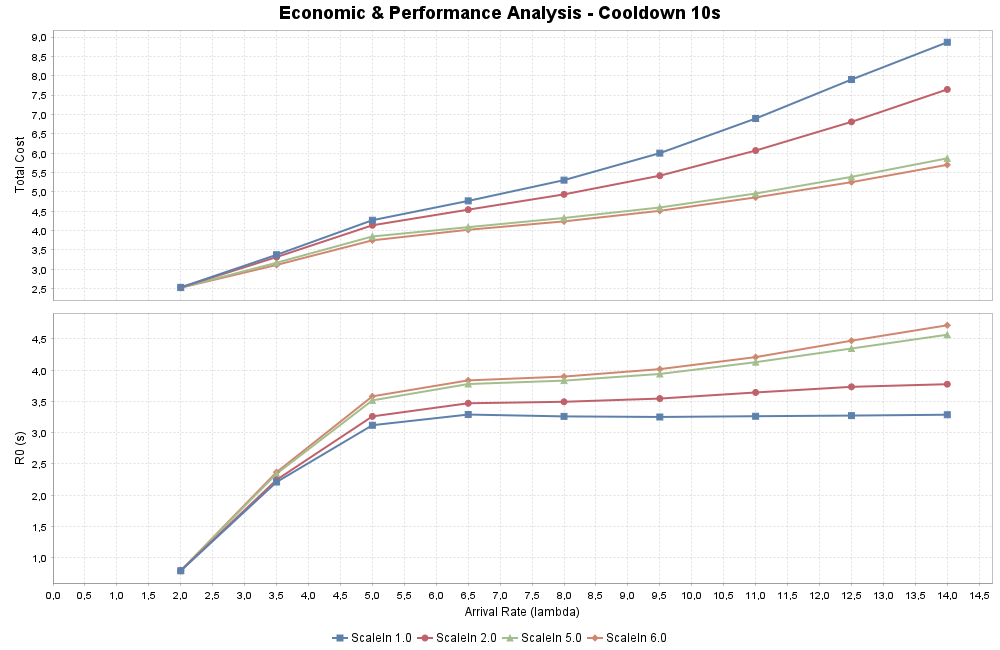
\includegraphics[width=0.72\textwidth]{../data/objective/cost/cost_analysis_cooldown_10s}
    \caption{Andamento del costo totale e del tempo medio di risposta con \textit{Cooldown} pari a $10\text{ s}$.}
    \label{fig:cost_analysis_cd10}
\end{figure}

\begin{figure}[H]
    \centering
    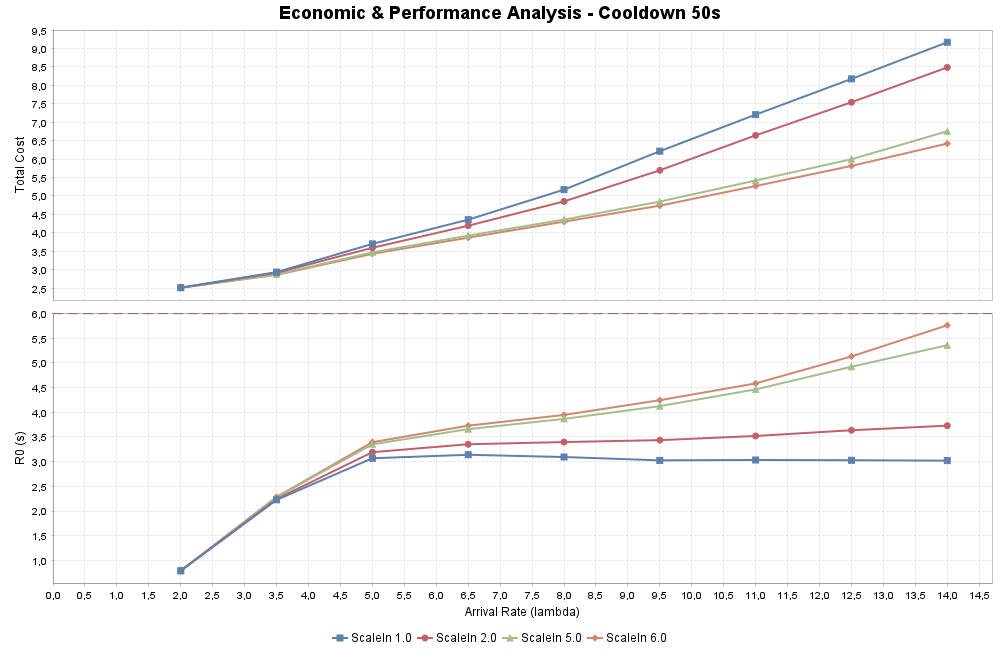
\includegraphics[width=0.72\textwidth]{../data/objective/cost/cost_analysis_cooldown_50s}
    \caption{Andamento del costo totale e del tempo medio di risposta con \textit{Cooldown} pari a $50\text{ s}$.}
    \label{fig:cost_analysis_cd50}
\end{figure}

\begin{figure}[H]
    \centering
    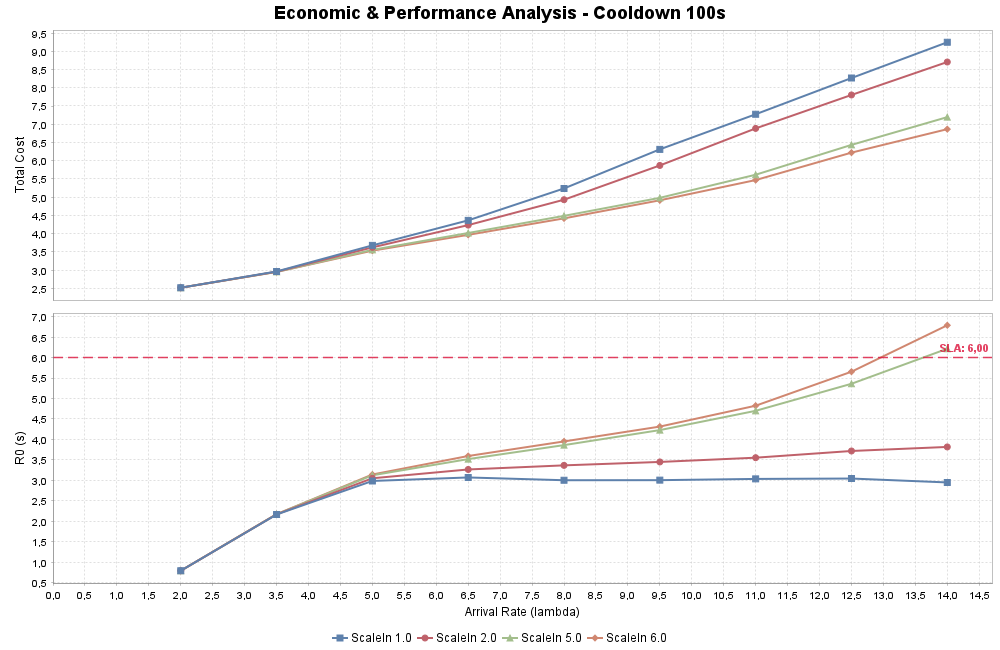
\includegraphics[width=0.72\textwidth]{../data/objective/cost/cost_analysis_cooldown_100s}
    \caption{Andamento del costo totale e del tempo medio di risposta con \textit{Cooldown} pari a $100\text{ s}$.}
    \label{fig:cost_analysis_cd100}
\end{figure}

Il \textit{Cooldown} ha un ruolo altrettanto rilevante. Un valore troppo breve, pari a $5\text{ s}$, rende il controller molto reattivo ma tende ad aumentare il costo medio: con $R^{min}=6.0\text{ s}$ il costo medio è $4.473$, contro $4.213$ ottenuto con $10\text{ s}$. Valori più lunghi riducono la frequenza delle riconfigurazioni, ma possono ritardare l'adattamento del cluster nei regimi più intensi: con $R^{min}=6.0\text{ s}$ e $\lambda=11$, il tempo medio di risposta passa da $4.2072\text{ s}$ con \textit{Cooldown} pari a $10\text{ s}$ a $4.5817\text{ s}$ con $50\text{ s}$ e $4.8231\text{ s}$ con $100\text{ s}$. D'altra parte, per soglie di \textit{Scale In} molto basse, un \textit{Cooldown} più lungo può anche ridurre leggermente la latenza media, perché mantiene la capacità orizzontale allocata più a lungo dopo un episodio di carico elevato.

Alla luce di queste evidenze, la configurazione economicamente più difendibile dipende dal profilo di carico atteso. Se si privilegia la robustezza prestazionale, $R^{min}=1.0\text{ s}$ o $R^{min}=2.0\text{ s}$ mantengono tempi di risposta più bassi, ma accettano un costo medio più elevato. Se invece l'obiettivo principale è contenere la spesa mantenendo il rispetto dello SLA, le configurazioni con $R^{min}=5.0\text{ s}$--$6.0\text{ s}$ sono più convenienti. Per le analisi successive si adotta quindi \textbf{\textit{Cooldown} pari a $10.0\text{ s}$}: tale valore preserva una buona reattività nei regimi ad alto carico, mantiene $R_0$ ben al di sotto dello SLA anche per $\lambda=11$ e riduce sensibilmente il costo rispetto al \textit{Cooldown} di $5\text{ s}$.

\paragraph{Analisi Transitoria a Orizzonte Finito}
L'analisi transitoria è stata condotta tramite la classe \texttt{TransientAnalysisObjective}. A differenza delle campagne steady-state, qui il sistema viene osservato a partire da uno stato iniziale vuoto, usando repliche indipendenti e salvando l'evoluzione temporale del tempo medio di risposta. Sono stati considerati sei scenari sulla sola architettura completa: due a basso carico, due a carico medio e due ad alto carico, variando sia $\lambda$ sia il coefficiente di variazione degli interarrivi. Ogni scenario è stato eseguito con $10$ repliche indipendenti; gli scenari low e medium sono stati simulati fino a circa $1008000\text{ s}$, mentre gli scenari high fino a $504000\text{ s}$, con scala temporale dei grafici convertita in ore per renderli leggibili.

\begin{table}[H]
    \centering
    \small
    \renewcommand{\arraystretch}{1.25}
    \begin{tabular}{lcccccc}
        \hline
        \textbf{Scenario} & \textbf{$\lambda$} & \textbf{$C_V$} & \textbf{$R_0$ [s]} & \textbf{HW [s]} & \textbf{$\bar{N}$} & \textbf{Util. Spike [\%]} \\ \hline
        Low CV2    & $2.5$ & $2.0$ & $0.8102$ & $0.0020$ & $1.0055$ & $0.00$ \\
        Low CV4    & $2.5$ & $4.0$ & $1.1721$ & $0.0049$ & $1.0466$ & $0.00$ \\
        Medium CV4 & $5.0$ & $4.0$ & $3.4218$ & $0.0041$ & $1.5707$ & $9.68$ \\
        Medium CV6 & $5.0$ & $6.0$ & $3.3204$ & $0.0062$ & $1.6710$ & $14.34$ \\
        High CV4   & $8.0$ & $4.0$ & $3.7118$ & $0.0031$ & $1.6274$ & $39.59$ \\
        High CV6   & $8.0$ & $6.0$ & $3.4832$ & $0.0047$ & $1.6581$ & $42.28$ \\ \hline
    \end{tabular}
    \caption{Risultati aggregati dell'analisi transitoria a orizzonte finito sulla configurazione completa.}
    \label{tab:transient_results}
\end{table}

La Tabella~\ref{tab:transient_results} mostra che il sistema rimane ampiamente sotto lo SLA in tutti gli scenari. L'obiettivo era verificare che, partendo da sistema vuoto, la configurazione completa non producesse transitori lunghi o derive iniziali capaci di falsare le conclusioni steady-state. Il risultato ottenuto è positivo: nei casi low load lo Spike Server rimane praticamente inutilizzato, con $\lambda=2.5$ e $C_V=2.0$ la media dei job deviati è prossima a zero e la latenza converge attorno a $0.81\text{ s}$; aumentando la variabilità a $C_V=4.0$ il tempo medio sale a $1.17\text{ s}$, ma l'architettura non richiede ancora un uso strutturale della risorsa di picco. Nei casi medium e high emerge invece la funzione gerarchica del sistema: il numero medio di server attivi cresce tra $1.57$ e $1.67$, mentre lo Spike Server assorbe una quota crescente dei burst, arrivando a utilizzazioni medie superiori al $40\%$ negli scenari high.

\begin{figure}[H]
    \centering
    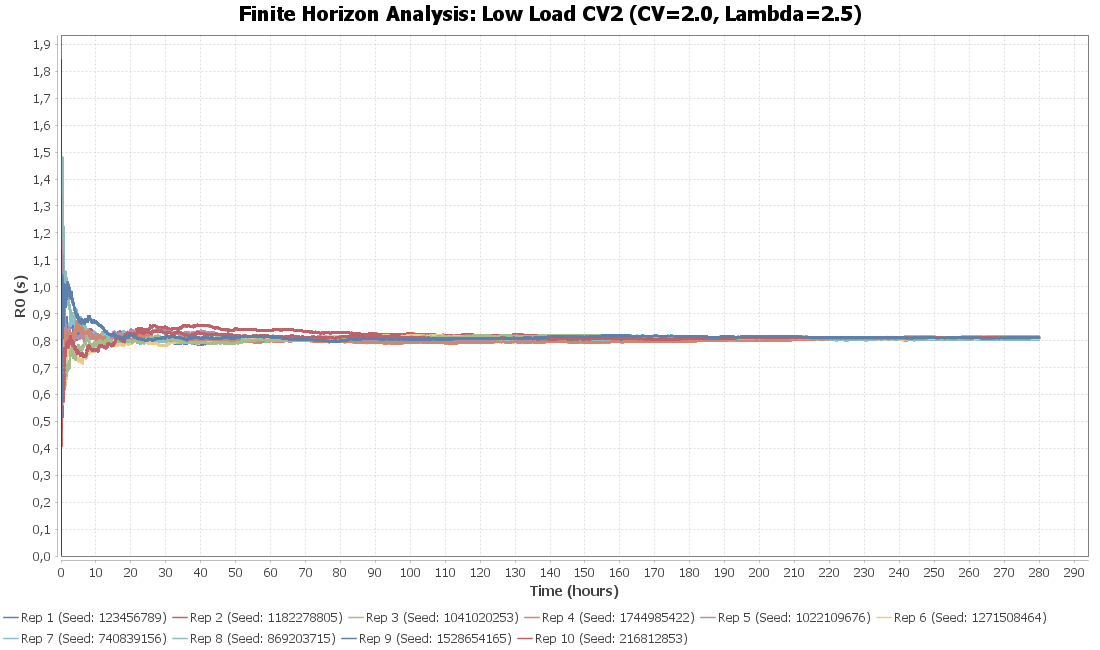
\includegraphics[width=0.95\textwidth]{../data/objective/finite/transient_low_load_cv2}
    \caption{Analisi transitoria dello scenario Low Load con $C_V=2.0$.}
    \label{fig:transient_low_cv2}
\end{figure}

\begin{figure}[H]
    \centering
    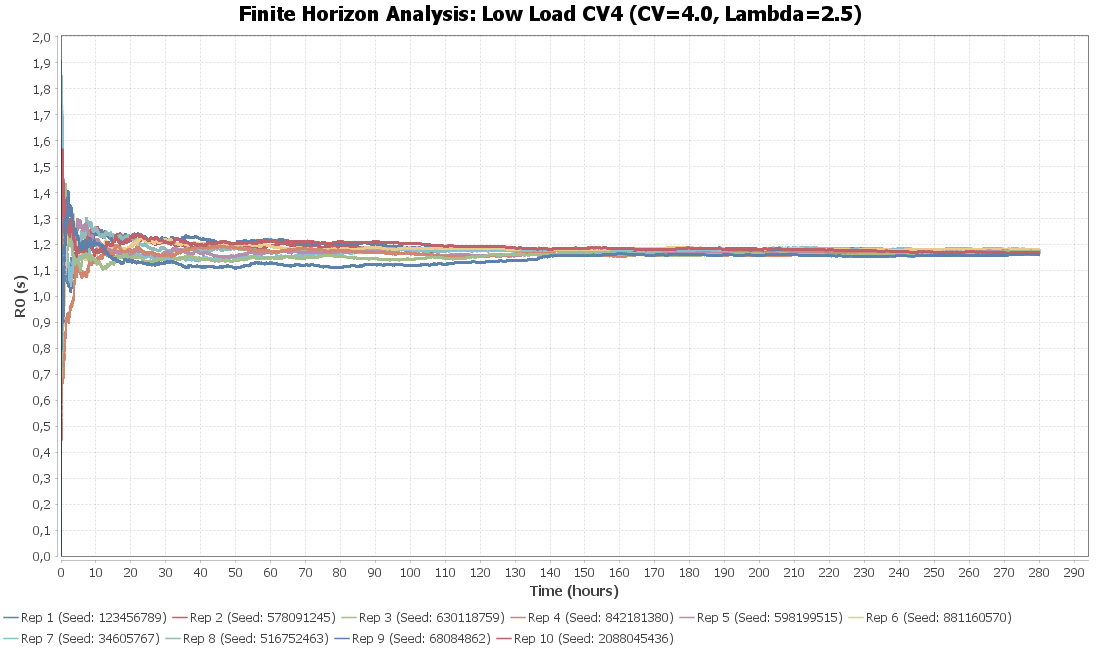
\includegraphics[width=0.95\textwidth]{../data/objective/finite/transient_low_load_cv4}
    \caption{Analisi transitoria dello scenario Low Load con $C_V=4.0$.}
    \label{fig:transient_low_cv4}
\end{figure}

\begin{figure}[H]
    \centering
    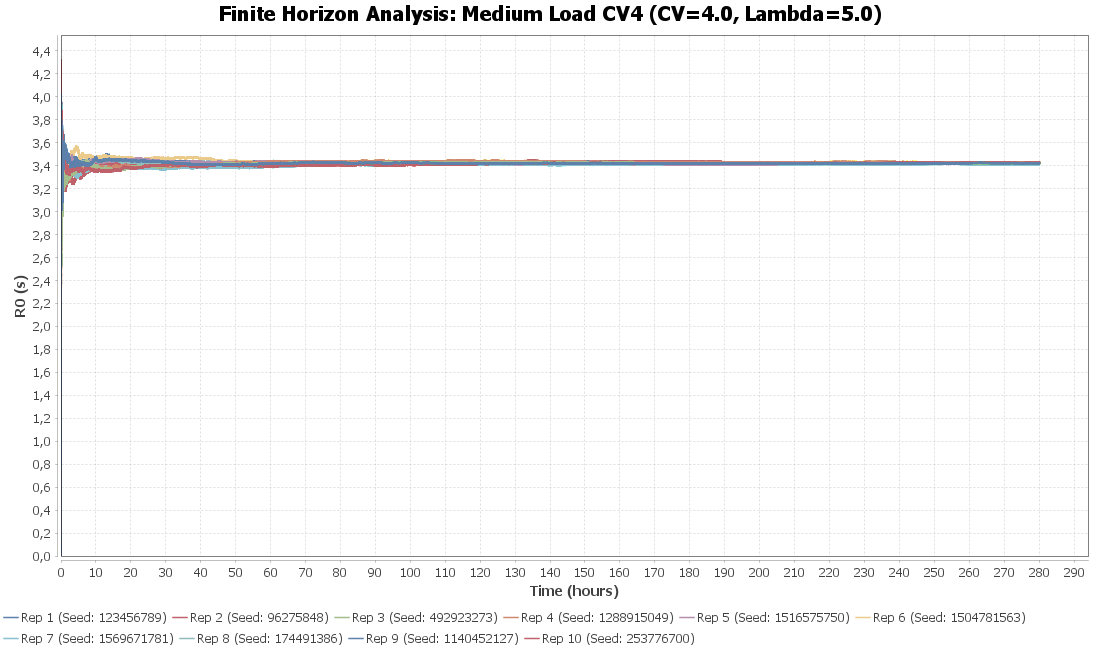
\includegraphics[width=0.74\textwidth]{../data/objective/finite/transient_medium_load_cv4}
    \caption{Analisi transitoria dello scenario Medium Load con $C_V=4.0$.}
    \label{fig:transient_medium_cv4}
\end{figure}

\begin{figure}[H]
    \centering
    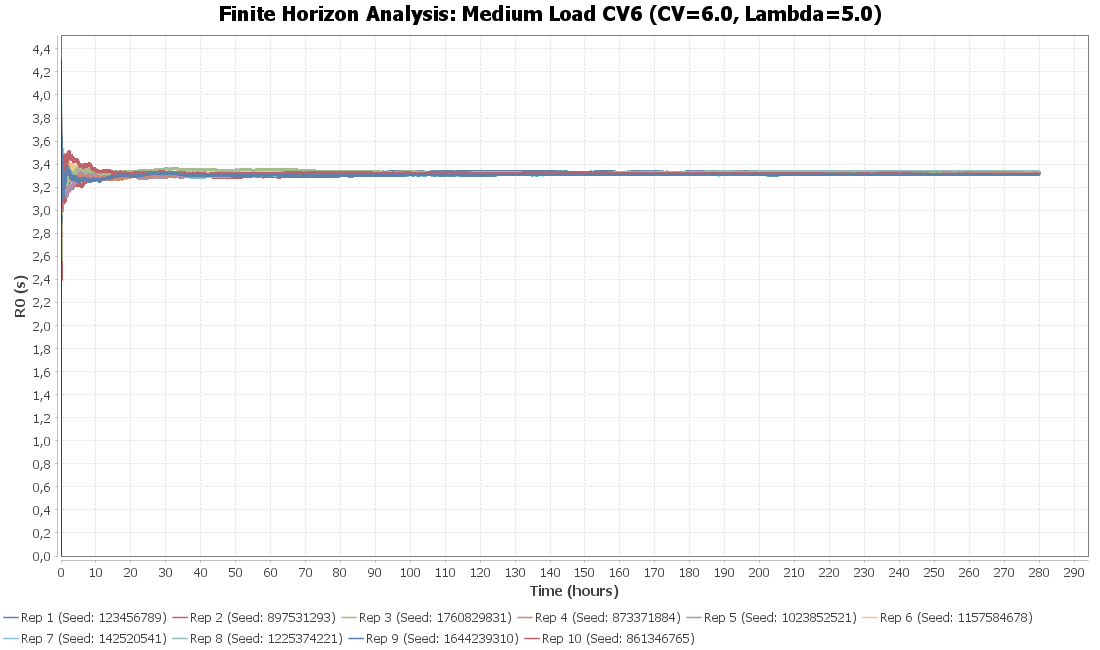
\includegraphics[width=0.74\textwidth]{../data/objective/finite/transient_medium_load_cv6}
    \caption{Analisi transitoria dello scenario Medium Load con $C_V=6.0$.}
    \label{fig:transient_medium_cv6}
\end{figure}

\begin{figure}[H]
    \centering
    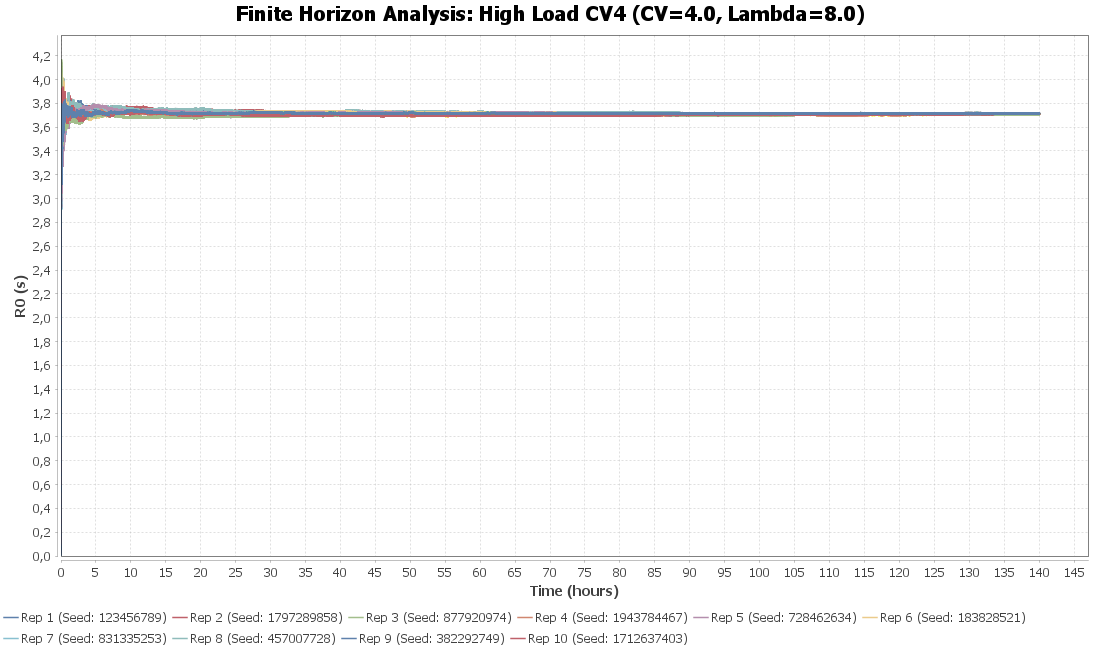
\includegraphics[width=0.74\textwidth]{../data/objective/finite/transient_high_load_cv4}
    \caption{Analisi transitoria dello scenario High Load con $C_V=4.0$.}
    \label{fig:transient_high_cv4}
\end{figure}

\begin{figure}[H]
    \centering
    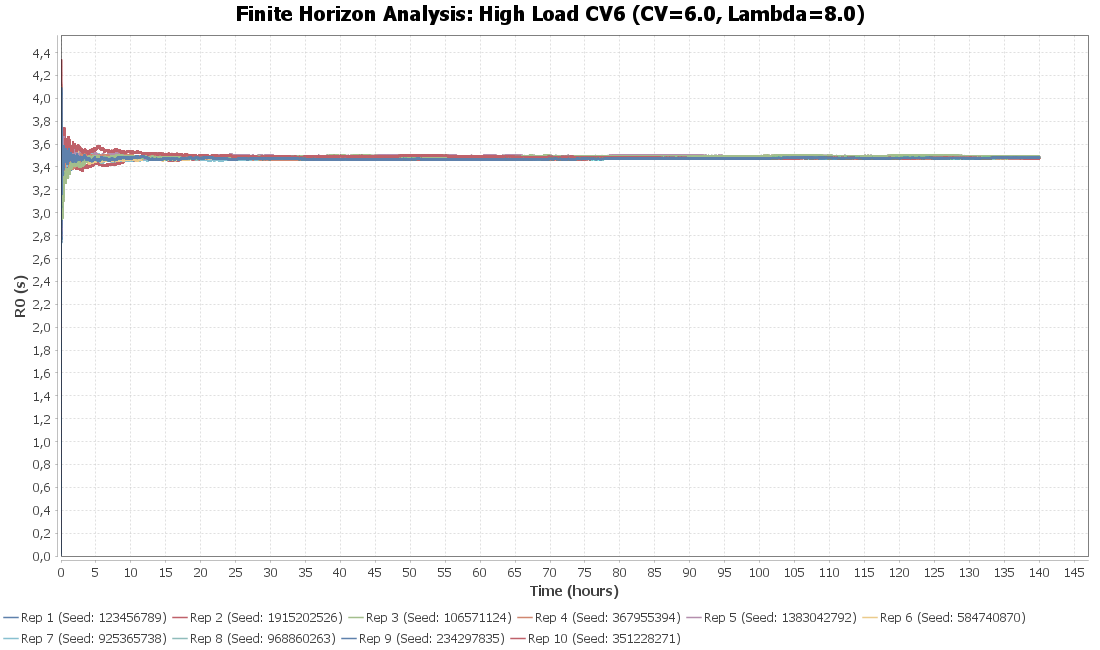
\includegraphics[width=0.74\textwidth]{../data/objective/finite/transient_high_load_cv6}
    \caption{Analisi transitoria dello scenario High Load con $C_V=6.0$.}
    \label{fig:transient_high_cv6}
\end{figure}

I grafici confermano che la fase iniziale non presenta derive instabili: dopo l'assestamento iniziale, le repliche oscillano attorno a livelli coerenti con le stime aggregate. L'aumento del coefficiente di variazione non produce necessariamente un peggioramento monotono della media finale, perché il sistema reagisce in modo diverso alla burstiness: quando i burst diventano più concentrati, una quota maggiore di traffico viene intercettata dal meccanismo di dirottamento e dallo scaling verticale, riducendo il carico residuo sui Web Server ordinari. Questo comportamento è particolarmente visibile negli scenari medium e high, dove l'aumento di $C_V$ fa crescere il numero di eventi di \textit{Scale Up} e l'utilizzazione dello Spike Server, ma mantiene $R_0$ in una regione sicura.

\paragraph{Robustezza alla Burstiness}
La robustezza del sistema rispetto alla variabilità degli interarrivi è stata analizzata tramite la classe \texttt{BurstinessRobustnessObjective}. La campagna usa la configurazione completa scelta nelle fasi precedenti e osserva, al variare di $\lambda$ e di $C_V$, non solo il tempo medio di risposta, ma anche job nel sistema, utilizzazione, throughput, job deviati, numero medio di server attivi e numero di azioni di scaling. La stima è stata condotta con $1024$ batch da $4096$ job, riportando per ogni metrica media, deviazione standard, \textit{Half-Width} e intervallo di confidenza al $95\%$. Il comportamento atteso è una maggiore attivazione delle risorse elastiche al crescere della burstiness, con possibile aumento della variabilità delle misure ma senza perdita di stabilità del tempo medio di risposta.

\begin{table}[H]
    \centering
    \small
    \renewcommand{\arraystretch}{1.2}
    \begin{tabular}{lcccccc}
        \hline
        \textbf{$C_V$} & \textbf{$\lambda$} & \textbf{$R_0$ [s]} & \textbf{HW [s]} & \textbf{JIS} & \textbf{$\bar{N}$} & \textbf{Util. Spike [\%]} \\ \hline
        $1.0$  & $5.0$  & $3.4204$ & $0.0214$ & $17.12$ & $1.61$ & $2.34$ \\
        $1.0$  & $11.0$ & $4.0110$ & $0.0167$ & $44.15$ & $1.68$ & $67.34$ \\
        $4.0$  & $5.0$  & $3.4064$ & $0.0167$ & $17.14$ & $1.56$ & $9.52$ \\
        $4.0$  & $11.0$ & $3.9478$ & $0.0182$ & $43.67$ & $1.76$ & $62.44$ \\
        $8.0$  & $5.0$  & $3.2196$ & $0.0163$ & $16.42$ & $1.83$ & $17.91$ \\
        $8.0$  & $11.0$ & $3.7171$ & $0.0227$ & $41.79$ & $2.03$ & $61.20$ \\
        $12.0$ & $5.0$  & $3.1388$ & $0.0195$ & $16.42$ & $2.33$ & $22.26$ \\
        $12.0$ & $11.0$ & $3.6265$ & $0.0312$ & $42.03$ & $2.57$ & $58.35$ \\ \hline
    \end{tabular}
    \caption{Sintesi della robustezza alla burstiness per alcuni punti rappresentativi.}
    \label{tab:burstiness_results}
\end{table}

La Tabella~\ref{tab:burstiness_results} evidenzia un risultato importante: l'incremento della burstiness non porta il sistema fuori controllo. Al contrario, a parità di $\lambda$, l'aumento di $C_V$ tende a far crescere l'uso delle risorse elastiche, ma mantiene il tempo medio di risposta in una regione più che accettabile rispetto allo SLA. Per $\lambda=11$, ad esempio, $R_0$ passa da $4.0110\text{ s}$ con $C_V=1.0$ a $3.6265\text{ s}$ con $C_V=12.0$; questo non significa che un traffico più bursty sia intrinsecamente più semplice, ma che il meccanismo di protezione intercetta più frequentemente i picchi e sposta lavoro verso lo Spike Server e verso configurazioni con più Web Server attivi.

\begin{figure}[H]
    \centering
    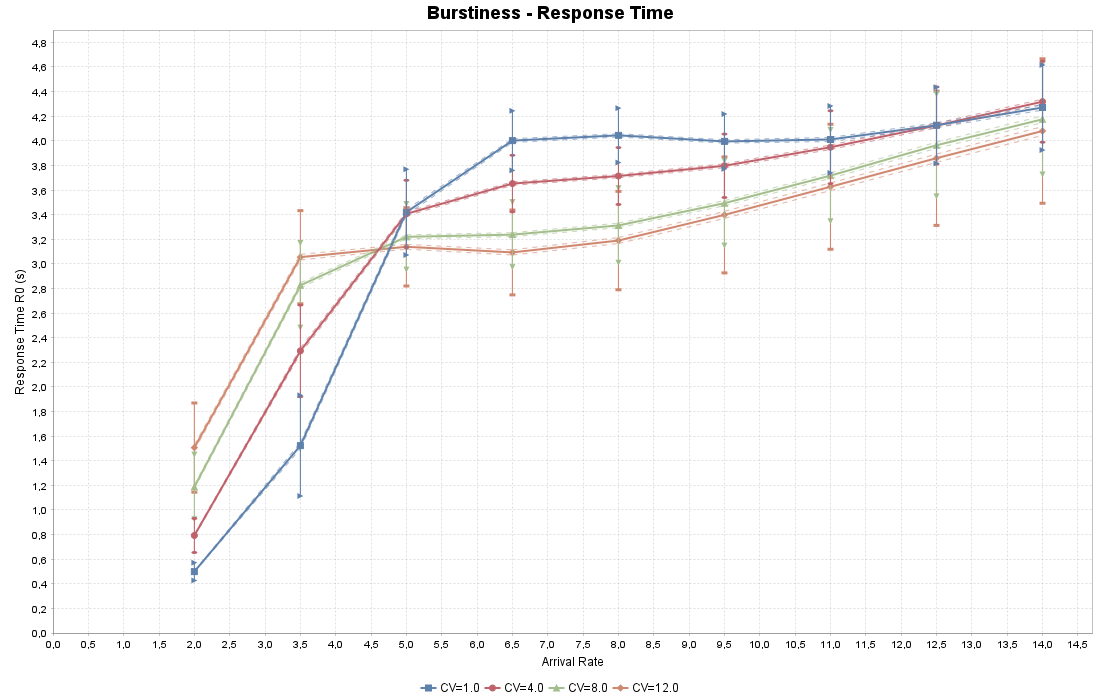
\includegraphics[width=0.76\textwidth]{../data/objective/burstiness/burstiness_robustness_response_time}
    \vspace{0.01\textheight}
    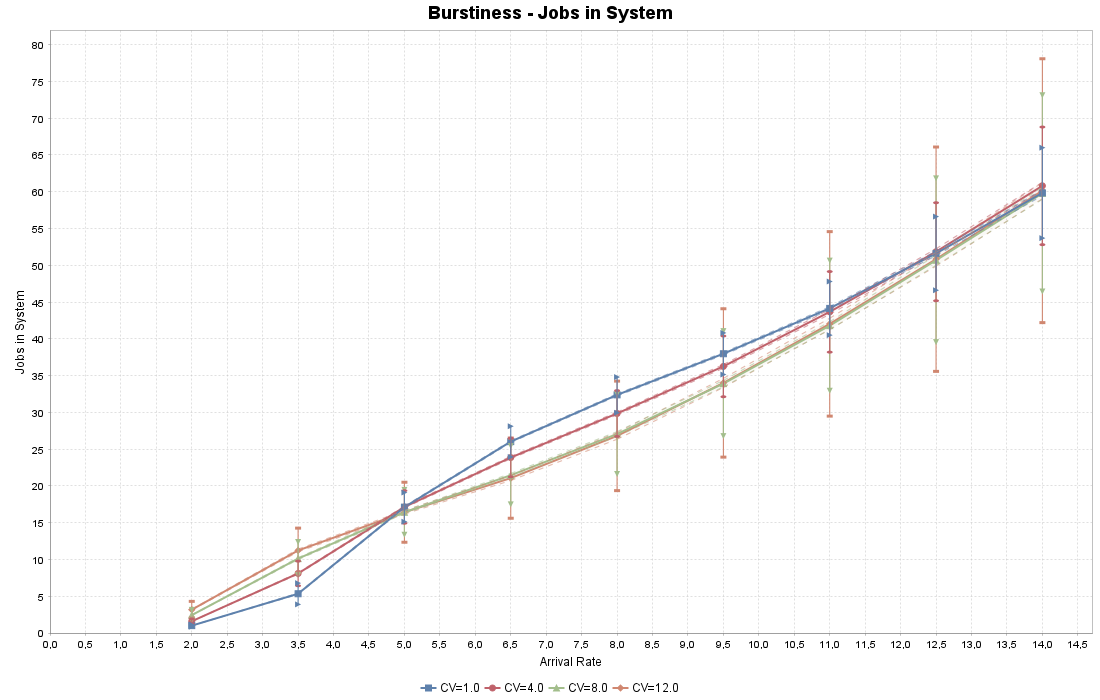
\includegraphics[width=0.76\textwidth]{../data/objective/burstiness/burstiness_robustness_jobs_in_system}
    \caption{Robustezza alla burstiness: tempo medio di risposta e numero medio di job nel sistema.}
    \label{fig:burstiness_rt_jis}
\end{figure}

\begin{figure}[H]
    \centering
    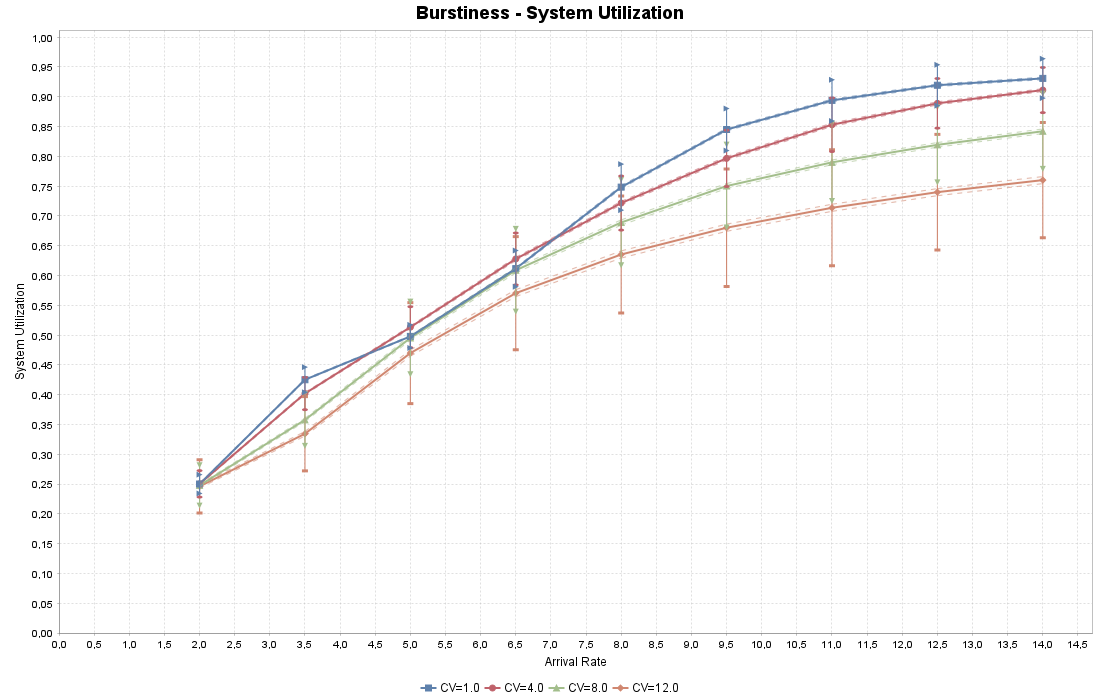
\includegraphics[width=0.76\textwidth]{../data/objective/burstiness/burstiness_robustness_system_utilization}
    \vspace{0.01\textheight}
    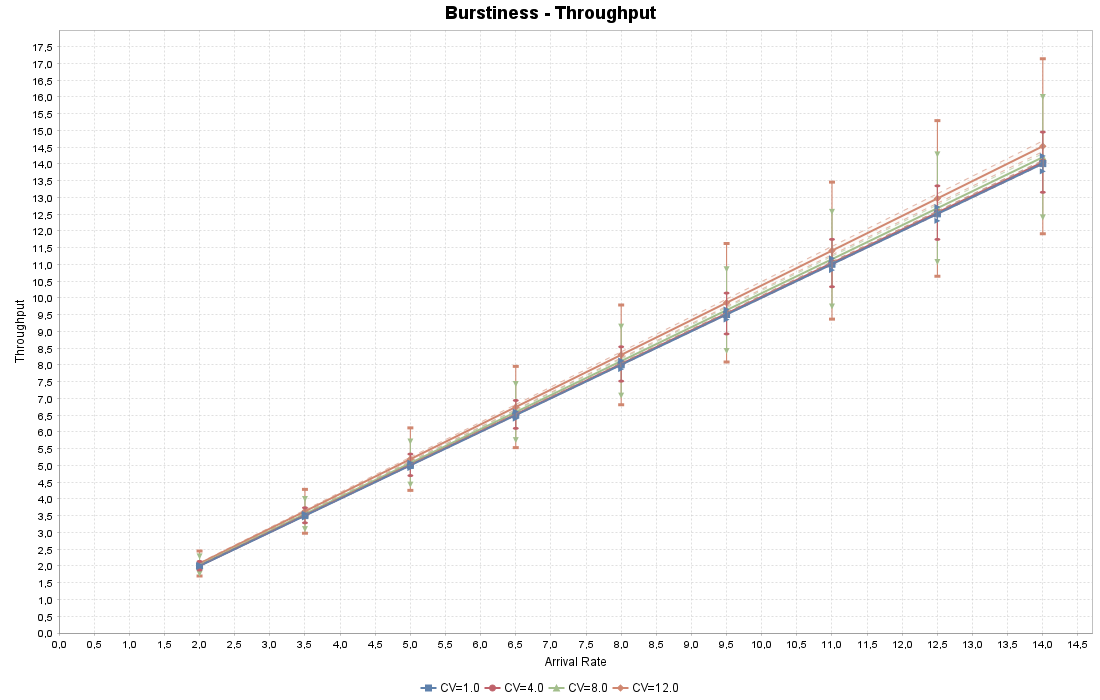
\includegraphics[width=0.76\textwidth]{../data/objective/burstiness/burstiness_robustness_throughput}
    \caption{Robustezza alla burstiness: utilizzazione complessiva del sistema e throughput.}
    \label{fig:burstiness_util_thr}
\end{figure}

\begin{figure}[H]
    \centering
    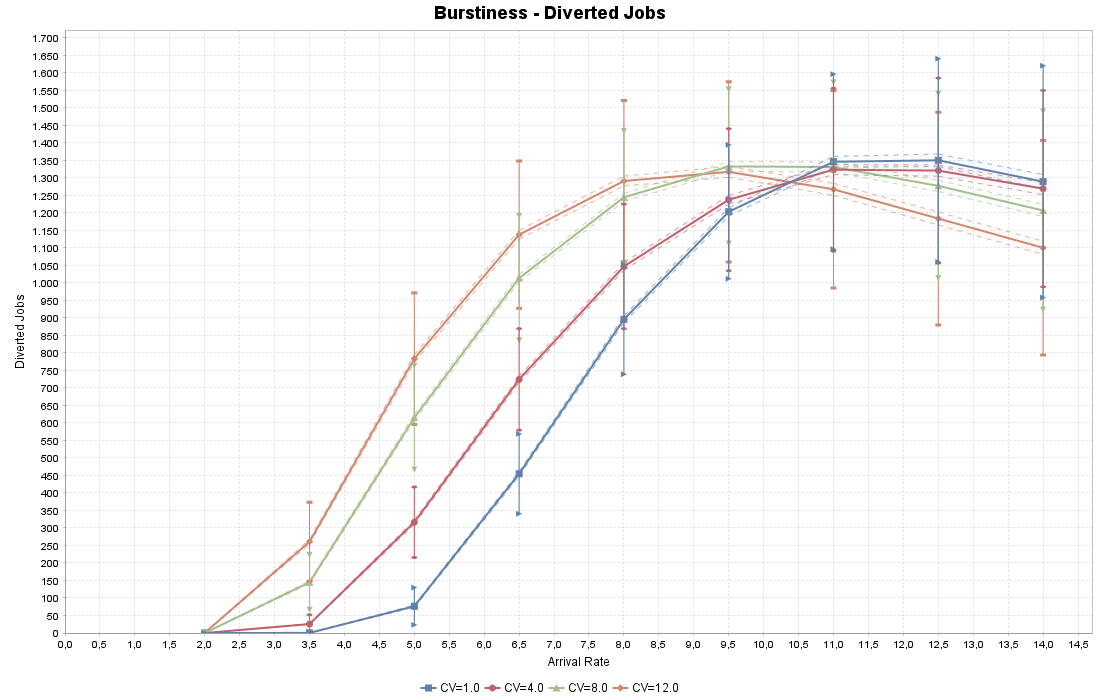
\includegraphics[width=0.76\textwidth]{../data/objective/burstiness/burstiness_robustness_diverted_jobs}
    \vspace{0.01\textheight}
    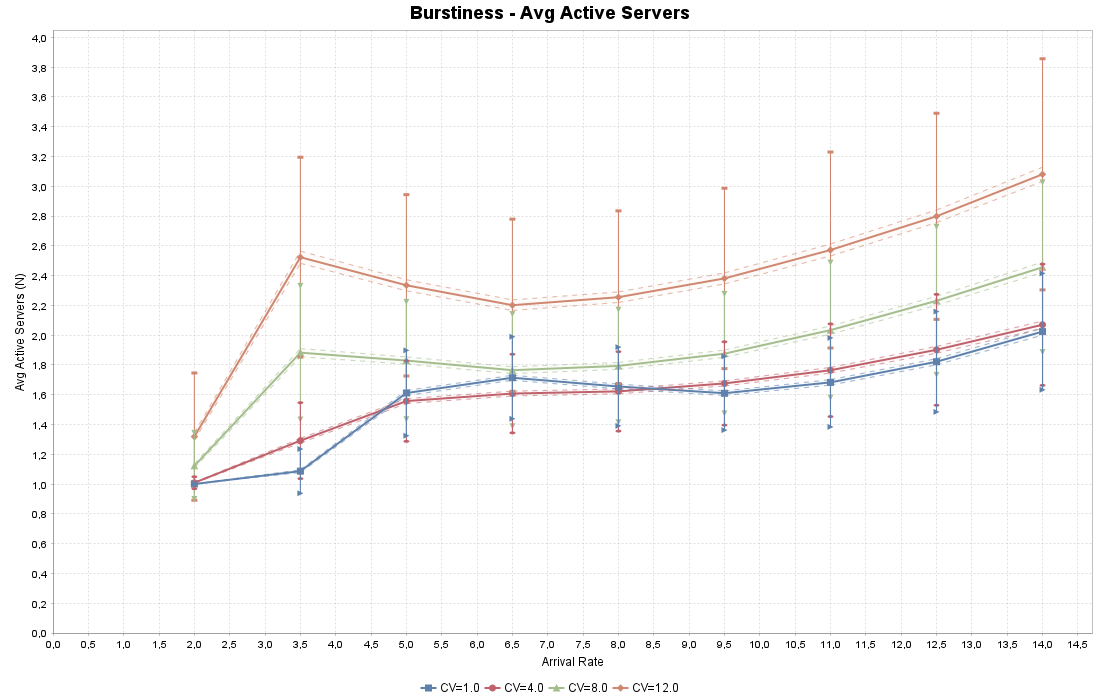
\includegraphics[width=0.76\textwidth]{../data/objective/burstiness/burstiness_robustness_avg_servers}
    \caption{Robustezza alla burstiness: job deviati e numero medio di Web Server attivi.}
    \label{fig:burstiness_diverted_servers}
\end{figure}

\begin{figure}[H]
    \centering
    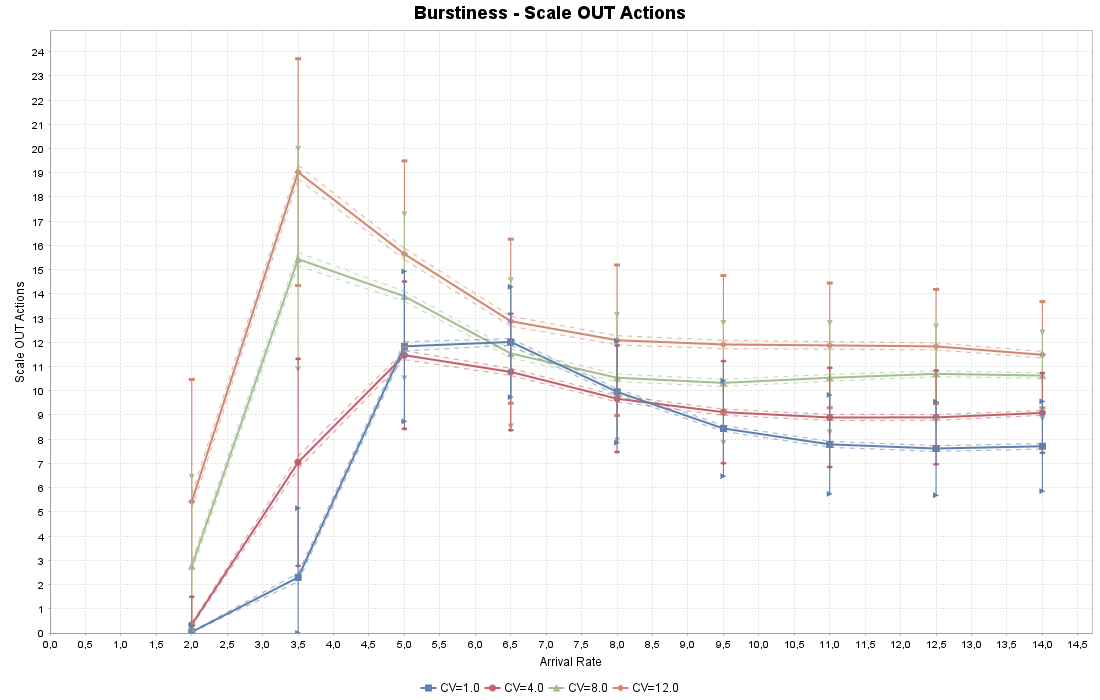
\includegraphics[width=0.76\textwidth]{../data/objective/burstiness/burstiness_robustness_scale_out_actions}
    \vspace{0.01\textheight}
    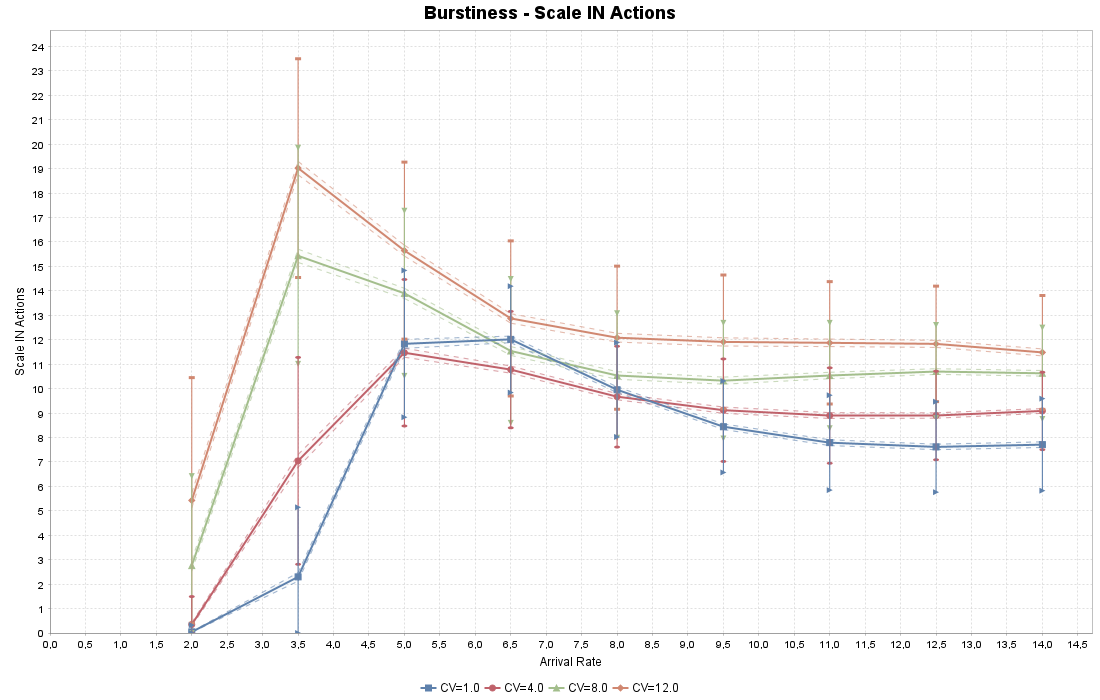
\includegraphics[width=0.76\textwidth]{../data/objective/burstiness/burstiness_robustness_scale_in_actions}
    \caption{Robustezza alla burstiness: azioni di \textit{Scale Out} e \textit{Scale In}.}
    \label{fig:burstiness_scale_horizontal}
\end{figure}

\begin{figure}[H]
    \centering
    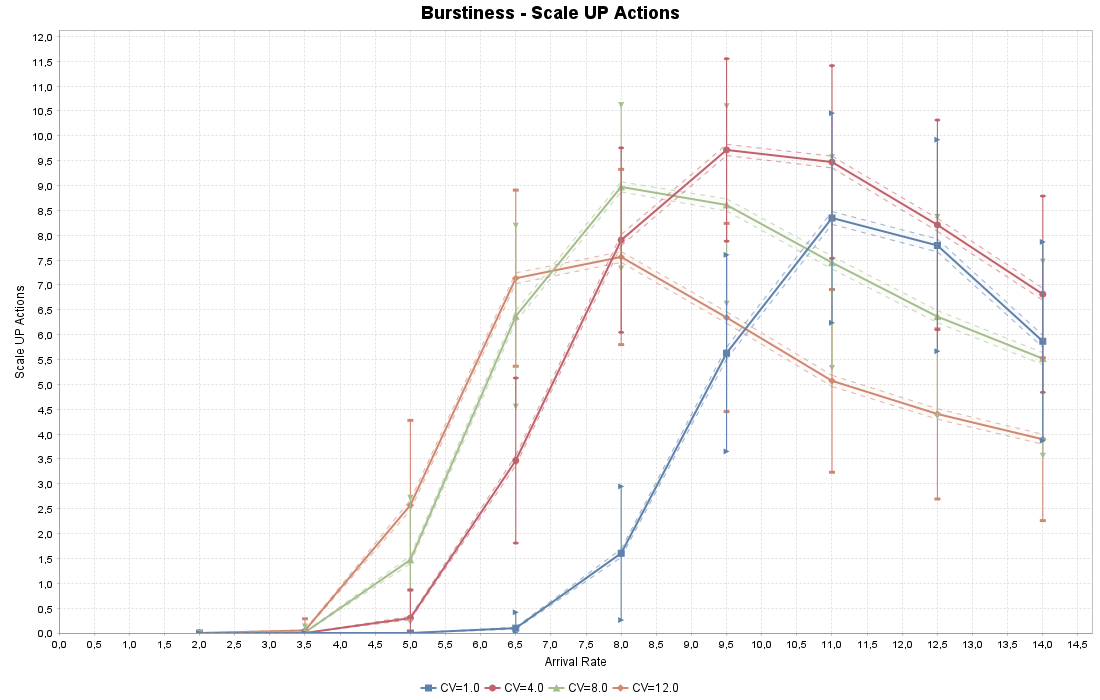
\includegraphics[width=0.76\textwidth]{../data/objective/burstiness/burstiness_robustness_scale_up_actions}
    \vspace{0.01\textheight}
    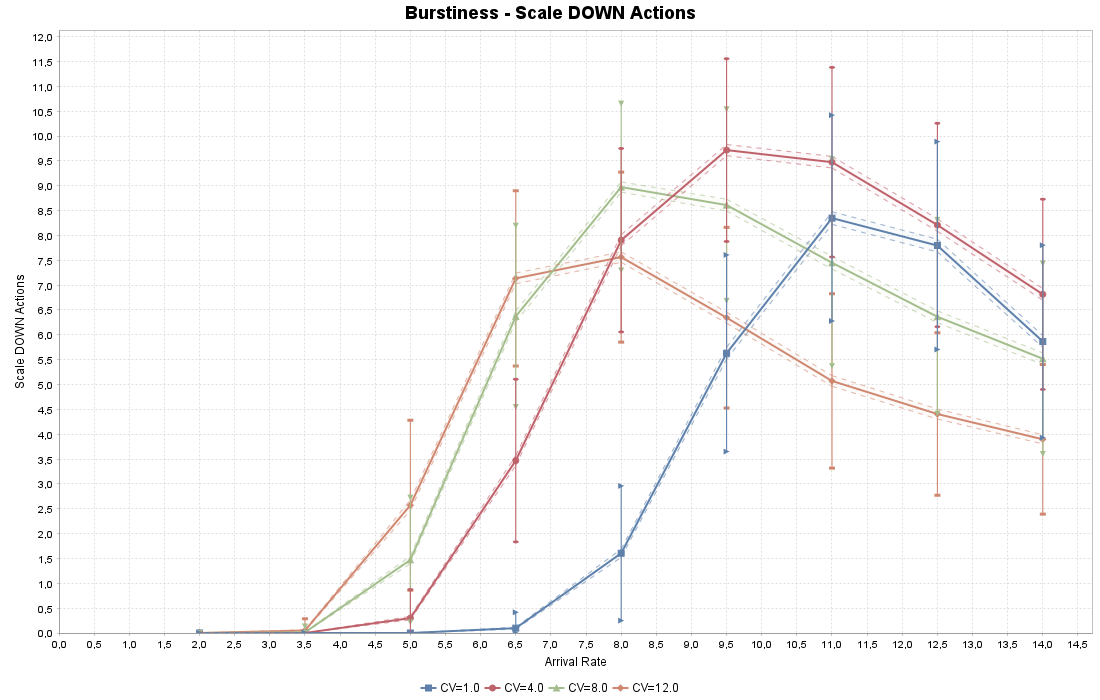
\includegraphics[width=0.76\textwidth]{../data/objective/burstiness/burstiness_robustness_scale_down_actions}
    \caption{Robustezza alla burstiness: azioni di \textit{Scale Up} e \textit{Scale Down}.}
    \label{fig:burstiness_scale_vertical}
\end{figure}

\begin{figure}[H]
    \centering
    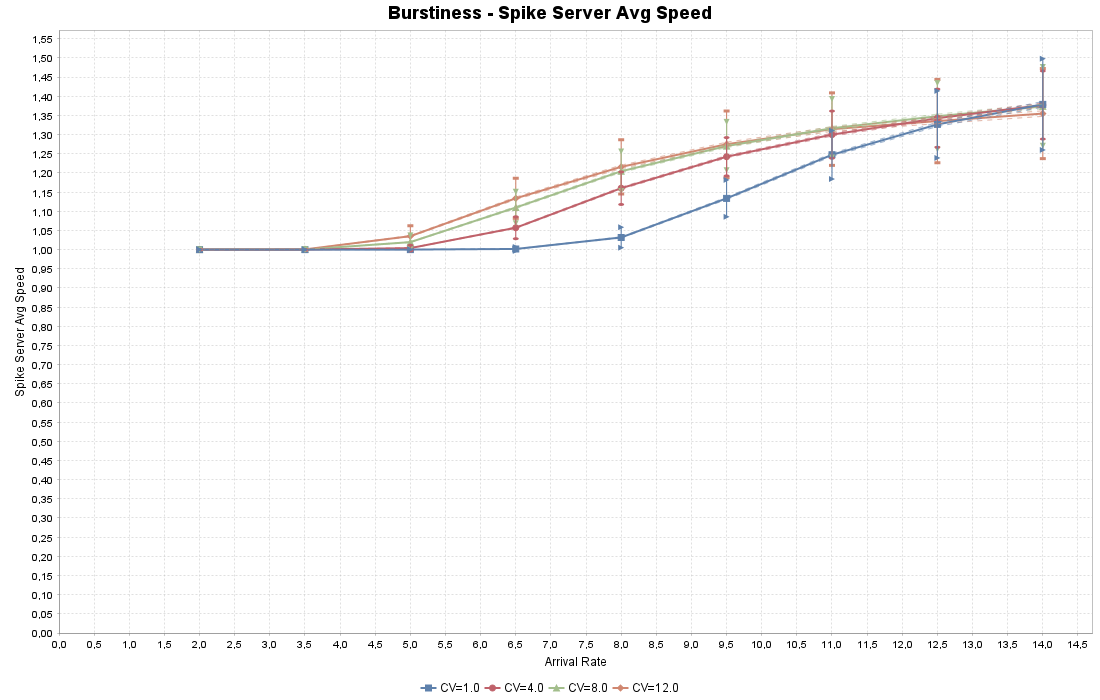
\includegraphics[width=0.76\textwidth]{../data/objective/burstiness/burstiness_robustness_spike_avg_speed}
    \vspace{0.01\textheight}
    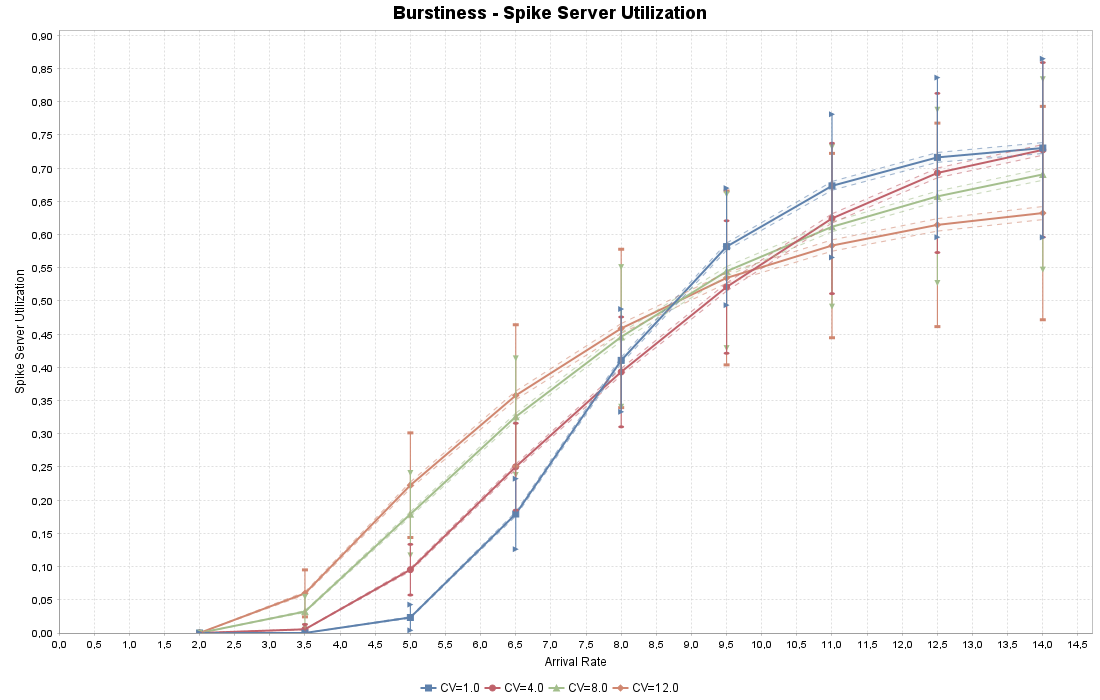
\includegraphics[width=0.76\textwidth]{../data/objective/burstiness/burstiness_robustness_spike_utilization}
    \caption{Robustezza alla burstiness: velocità media e utilizzazione dello Spike Server.}
    \label{fig:burstiness_spike}
\end{figure}

Le figure confermano la natura adattiva dell'architettura. Il throughput segue correttamente il tasso di arrivo, segnalando assenza di perdita strutturale di capacità; il numero di job nel sistema cresce con $\lambda$, ma resta compatibile con tempi medi di risposta sotto soglia; le azioni di scaling aumentano nelle regioni più intense, ma non producono divergenze. La presenza delle barre di deviazione standard e del contorno dell'intervallo di confidenza permette inoltre di distinguere il rumore statistico dalle tendenze effettive: le curve restano separate soprattutto per le metriche operative, mentre il tempo di risposta mostra intervalli contenuti rispetto al margine disponibile sullo SLA.

\subsection{Miglioramento}

\paragraph{Ottimizzazione Avanzata: Meccanismo a Bande di Isteresi}
L'ultimo obiettivo analizza il possibile miglioramento del meccanismo di dirottamento verso lo Spike Server introducendo una banda di isteresi sullo \textit{Spike Indicator}. La classe \texttt{VerticalScalerStabilityObjective} confronta quattro ampiezze di banda, pari a $0$, $5$, $10$ e $20$, mantenendo fisso $SI_{max}=40$ e variando $\lambda$ e il coefficiente di variazione degli interarrivi. Una banda nulla corrisponde alla soglia rigida: il traffico viene dirottato solo quando il server supera la soglia superiore e il rilascio avviene immediatamente appena il valore torna sotto soglia. Le bande positive introducono invece una soglia inferiore $SI_{low}$, stabilizzando la decisione del router. L'attesa progettuale è che bande più ampie riducano l'intermittenza del controllo, migliorando la regolarità del tempo di risposta, ma aumentando l'utilizzo medio dello Spike Server.

L'obiettivo non è ridurre indiscriminatamente l'uso dello Spike Server, ma rendere più regolare il suo impiego. Con una soglia rigida, infatti, il sistema tende ad alternare rapidamente fasi di dirottamento e fasi di ritorno al Web Server ordinario, specialmente quando il numero di job residenti oscilla vicino a $SI_{max}$. Questa dinamica può generare \textit{chattering}: molte decisioni ravvicinate, poco informative e potenzialmente costose. Una banda più ampia evita che il router cambi stato per oscillazioni marginali, accettando una maggiore permanenza del traffico sullo Spike Server in cambio di una risposta più stabile.

\begin{table}[H]
    \centering
    \small
    \renewcommand{\arraystretch}{1.2}
    \begin{tabular}{lcccc}
        \hline
        \textbf{Banda} & \textbf{$R_0$ a $\lambda=5,C_V=4$} & \textbf{Util. Spike [\%]} & \textbf{$R_0$ a $\lambda=11,C_V=4$} & \textbf{Util. Spike [\%]} \\ \hline
        $0$  & $3.406$ & $9.5$  & $3.948$ & $62.4$ \\
        $5$  & $3.360$ & $10.6$ & $3.899$ & $65.5$ \\
        $10$ & $3.312$ & $11.7$ & $3.846$ & $68.2$ \\
        $20$ & $3.177$ & $13.5$ & $3.758$ & $74.5$ \\ \hline
    \end{tabular}
    \caption{Effetto della banda di isteresi sul tempo di risposta e sull'utilizzazione dello Spike Server per $C_V=4.0$.}
    \label{tab:band_results}
\end{table}

I risultati in Tabella~\ref{tab:band_results} mostrano un miglioramento progressivo del tempo medio di risposta al crescere della banda. Per $C_V=4.0$ e $\lambda=5$, $R_0$ passa da $3.406\text{ s}$ con banda nulla a $3.177\text{ s}$ con banda pari a $20$, mentre per $\lambda=11$ passa da $3.948\text{ s}$ a $3.758\text{ s}$. Il prezzo pagato è un aumento dell'utilizzazione dello Spike Server, che nello scenario a $\lambda=11$ sale dal $62.4\%$ al $74.5\%$. Il comportamento è quindi coerente con l'interpretazione di progetto: la banda non elimina il costo della protezione, ma lo trasforma in un uso più continuo e meno intermittente della risorsa ausiliaria.

\begin{figure}[H]
    \centering
    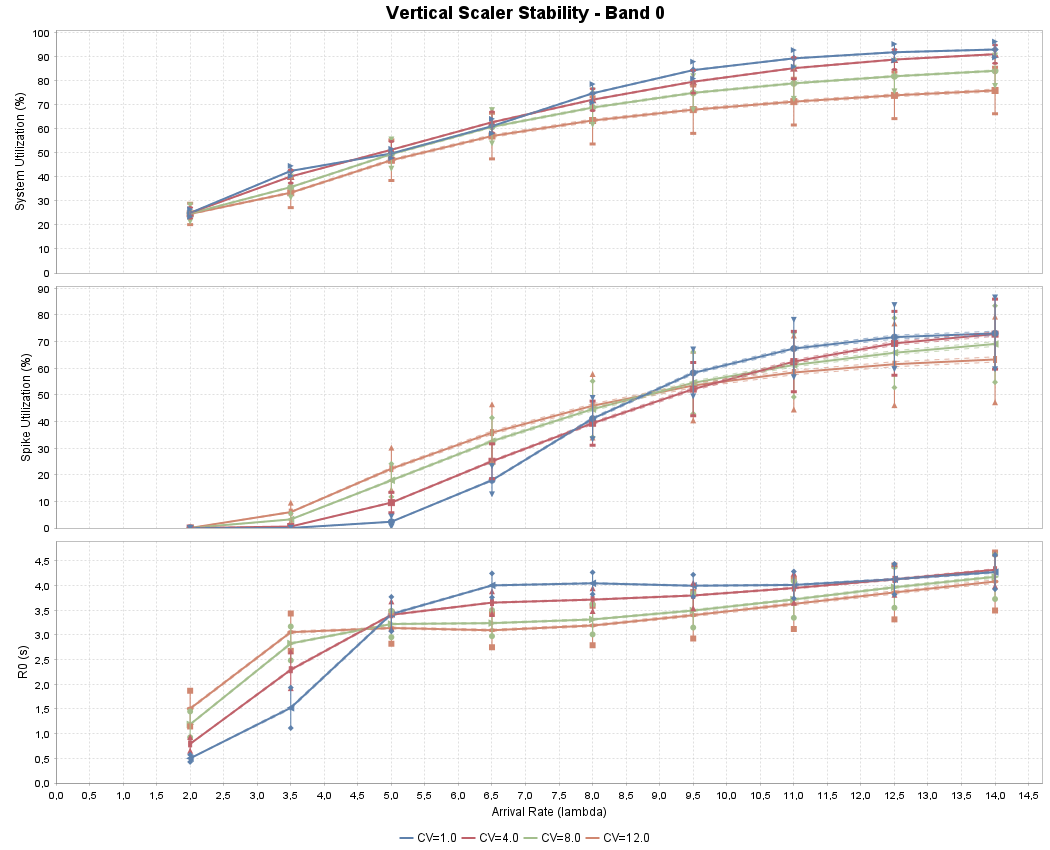
\includegraphics[width=0.72\textwidth]{../data/objective/band/vertical_scaler_stability_band_0}
    \caption{Stabilità dello scaler verticale e prestazioni con banda di isteresi pari a $0$.}
    \label{fig:band_0}
\end{figure}

\begin{figure}[H]
    \centering
    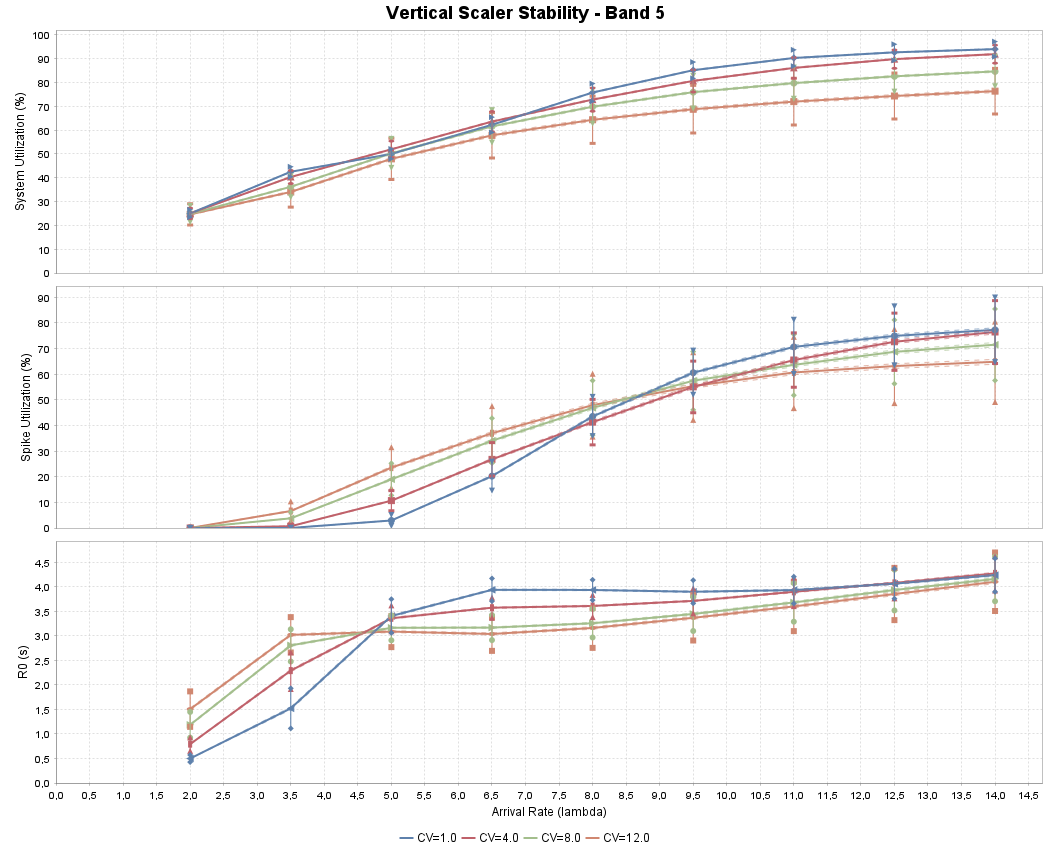
\includegraphics[width=0.72\textwidth]{../data/objective/band/vertical_scaler_stability_band_5}
    \caption{Stabilità dello scaler verticale e prestazioni con banda di isteresi pari a $5$.}
    \label{fig:band_5}
\end{figure}

\begin{figure}[H]
    \centering
    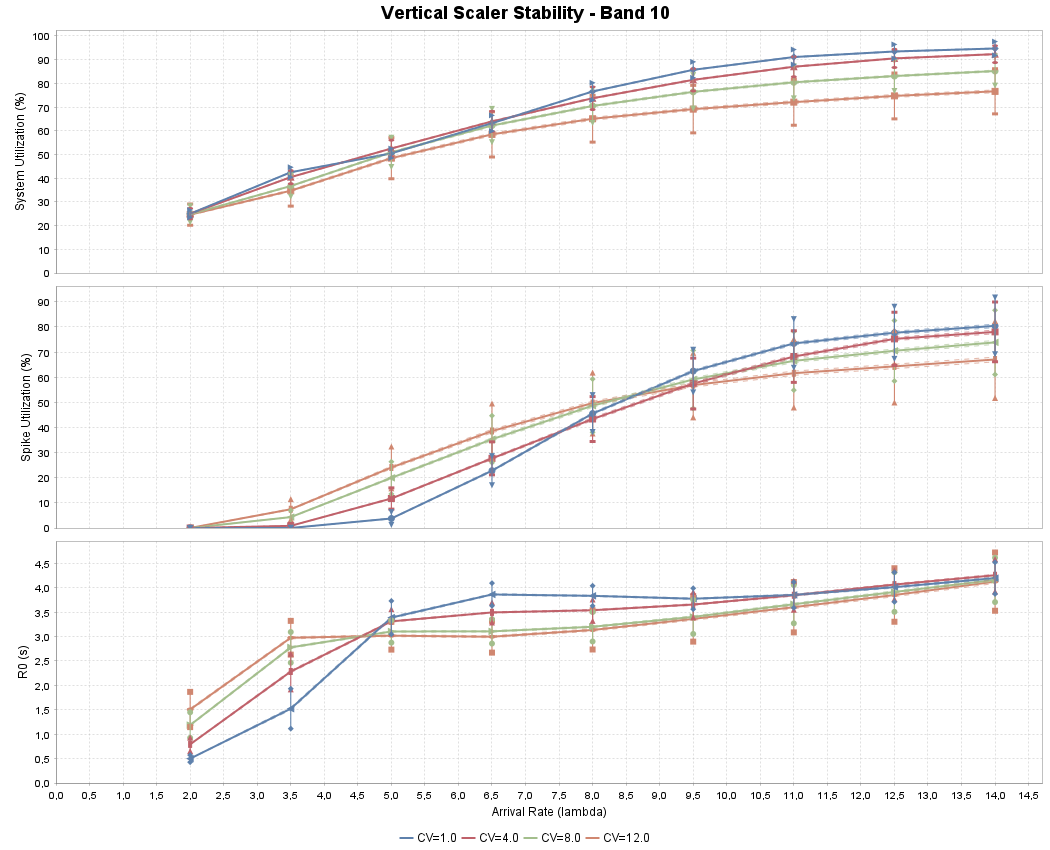
\includegraphics[width=0.72\textwidth]{../data/objective/band/vertical_scaler_stability_band_10}
    \caption{Stabilità dello scaler verticale e prestazioni con banda di isteresi pari a $10$.}
    \label{fig:band_10}
\end{figure}

\begin{figure}[H]
    \centering
    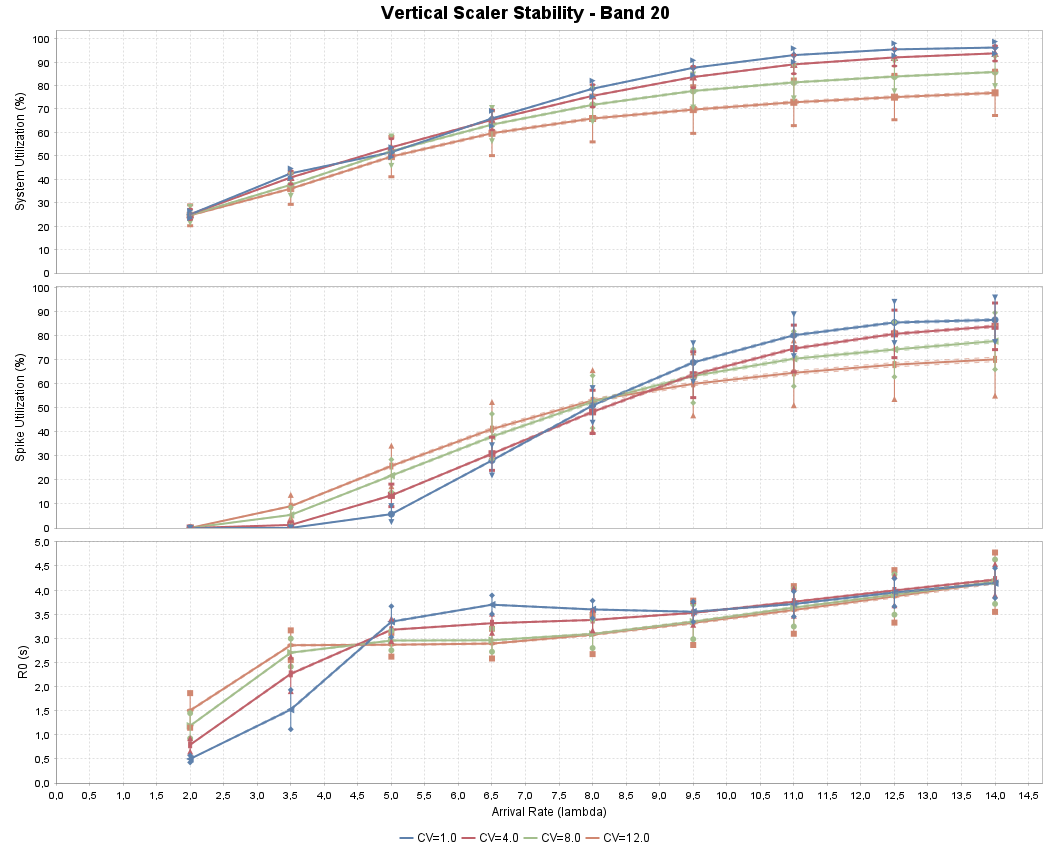
\includegraphics[width=0.72\textwidth]{../data/objective/band/vertical_scaler_stability_band_20}
    \caption{Stabilità dello scaler verticale e prestazioni con banda di isteresi pari a $20$.}
    \label{fig:band_20}
\end{figure}

Le Figure~\ref{fig:band_0}--\ref{fig:band_20} completano l'analisi mostrando tre curve per ciascuna banda: utilizzazione complessiva del sistema, utilizzazione dello Spike Server e tempo medio di risposta. L'aumento della banda rende più alta la curva di utilizzazione dello Spike Server, soprattutto nei regimi ad alta intensità, ma al tempo stesso abbassa la curva di $R_0$ e ne rende più regolare l'andamento. La banda pari a $20$ è la più aggressiva e fornisce i tempi di risposta più bassi, ma sposta una quota maggiore di costo operativo sulla risorsa di picco; una banda intermedia, pari a $10$, rappresenta invece un compromesso molto equilibrato, perché produce una riduzione visibile della latenza rispetto alla soglia rigida senza saturare eccessivamente lo Spike Server.

\section{Conclusioni}
Il lavoro svolto ha permesso di costruire, verificare e utilizzare un simulatore a eventi discreti per lo studio di un'infrastruttura cloud con autoscaling gerarchico. La verifica interna ha mostrato la coerenza del simulatore rispetto ai casi analitici noti, mentre la validazione esterna con JSIM ha confermato che il modello implementato riproduce correttamente sia il comportamento di una singola stazione ad alta variabilità sia l'effetto aggregato dell'architettura Web Server--Spike Server. Le differenze residue osservate nella validazione sono rimaste contenute e spiegabili dalle diverse astrazioni necessarie per rappresentare il routing a soglia nel simulatore del libro.

Dal punto di vista del dimensionamento, il risultato più netto riguarda il ruolo della politica di routing. La strategia \textit{Least Loaded} è risultata la più efficace, con $R_0=0.2843\text{ s}$ nello scenario statico a quattro Web Server, superando sia \textit{Round Robin} sia \textit{Power of Two Choices}. Questo conferma che, anche con disciplina \textit{Processor Sharing}, la distribuzione istantanea dei job tra i server resta decisiva: ridurre la congestione locale significa migliorare simultaneamente media e dispersione dei tempi di risposta.

La soglia di dirottamento $SI_{max}$ si è rivelata il parametro centrale per bilanciare protezione prestazionale e costo operativo della risorsa ausiliaria. La scelta $SI_{max}=40$ è risultata il miglior punto prima della violazione dello SLA: a tale valore il sistema mantiene $R_0=5.5279\text{ s}$ con intervallo di confidenza interamente sotto $6\text{ s}$, mentre a $SI_{max}=50$ la latenza supera già il vincolo. L'analisi dello speedup verticale ha invece mostrato che incrementi più aggressivi della velocità dello Spike Server non portano benefici apprezzabili; per questo motivo è stato scelto un incremento pari a $1.0$, cioè un raddoppio della capacità nel momento di attivazione.

Lo scaling orizzontale completa il controllo sul lungo periodo. La soglia superiore $R^{max}=6.0\text{ s}$ è stata mantenuta coincidente con il vincolo SLA, mentre $R^{min}=3.5\text{ s}$ è risultata coerente con uno scenario nominale centrato su $\lambda\simeq 5$. Le analisi di frontiera mostrano però che questa scelta non è universale: in presenza di carichi persistentemente elevati, prossimi a $\lambda=9.5$ o $\lambda=11$, è preferibile abbassare la soglia di \textit{Scale In} nell'intervallo $1.5$--$2.0\text{ s}$, accettando un maggior costo infrastrutturale in cambio di più margine operativo.

L'analisi economica ha quantificato in modo esplicito il compromesso tra costo e prestazioni. Con \textit{Cooldown} pari a $10\text{ s}$, le soglie di \textit{Scale In} più permissive, come $5.0$ e $6.0\text{ s}$, riducono il costo medio rispettivamente a $4.302$ e $4.213$, mantenendo comunque il tempo medio di risposta sotto SLA anche a $\lambda=11$. Soglie più aggressive, come $1.0$ e $2.0\text{ s}$, garantiscono latenze inferiori ma richiedono un numero medio maggiore di server attivi. Il \textit{Cooldown} pari a $10\text{ s}$ è emerso come scelta ragionevole perché evita sia l'iper-reattività del caso a $5\text{ s}$ sia l'eccessivo ritardo di adattamento osservabile nei casi a $50$ e $100\text{ s}$.

Le analisi transitorie e di burstiness mostrano la robustezza dell'architettura completa. Partendo da sistema vuoto, tutti i sei scenari a orizzonte finito convergono a tempi medi di risposta ampiamente inferiori allo SLA, anche quando il coefficiente di variazione degli interarrivi aumenta. In regime stazionario, la burstiness non produce instabilità: il sistema reagisce aumentando il ricorso allo Spike Server e alle azioni di scaling, mantenendo però $R_0$ in una regione controllata. Questo comportamento conferma l'efficacia della gerarchia: lo scaling orizzontale assorbe le variazioni strutturali del carico, mentre lo Spike Server protegge i Web Server ordinari dai burst locali che si sviluppano su scala temporale più rapida.

Infine, il meccanismo a bande di isteresi rappresenta il miglioramento più interessante dal punto di vista del controllo. La soglia rigida funziona, ma può generare decisioni intermittenti vicino al limite. L'introduzione di una banda riduce il \textit{chattering}, rende più continuo l'uso dello Spike Server e abbassa il tempo medio di risposta. Una banda pari a $20$ massimizza il beneficio prestazionale, ma aumenta sensibilmente l'utilizzazione della risorsa di picco; una banda pari a $10$ appare quindi come compromesso progettuale più equilibrato, perché migliora la stabilità senza spostare eccessivamente il costo sulla componente verticale.

In sintesi, l'architettura gerarchica proposta risulta efficace perché separa correttamente le scale temporali del problema: routing e Spike Server agiscono come protezione immediata contro i picchi, mentre lo scaling orizzontale governa il dimensionamento strutturale del cluster. Il simulatore sviluppato consente di quantificare questo equilibrio e fornisce linee guida operative precise: \textit{Least Loaded} come politica di routing, $SI_{max}=40$, incremento verticale pari a $1.0$, $R^{max}=6.0\text{ s}$, $R^{min}=3.5\text{ s}$ per il carico nominale, \textit{Cooldown} pari a $10\text{ s}$ e banda di isteresi preferibilmente intermedia. Queste scelte permettono di rispettare lo SLA con margine, contenendo al tempo stesso il costo operativo e mantenendo stabile il comportamento dinamico del sistema.

\newpage


\begin{thebibliography}{9}

\bibitem{leemis-park}
L. M. Leemis and S. K. Park, 
\textit{Discrete-Event Simulation: A First Course}, 
Pearson Prentice Hall, 2006.

\bibitem{serazzi-jmt-book}
G. Serazzi, 
\textit{Performance Engineering: Learning Through Applications Using JMT}, 
Springer Nature Switzerland AG, 2024.

\bibitem{jmt-software}
G. Serazzi, M. Gribaudo, G. Casale, et al., 
``Java Modelling Tools - JMT'', open-source suite, 
\url{http://jmt.sourceforge.net/}.

\bibitem{harchol-balter}
M. Harchol-Balter, 
\textit{Performance Modeling and Design of Computer Systems: Queueing Theory in Action}, 
Cambridge University Press, 2013.

\bibitem{park-miller}
S. K. Park and K. W. Miller, 
``Random Number Generators: Good Ones Are Hard To Find'', 
\textit{Communications of the ACM}, Vol. 31, No. 10, pp. 1192-1201, 1988.

\end{thebibliography}

\end{document}










